% Options for packages loaded elsewhere
\PassOptionsToPackage{unicode}{hyperref}
\PassOptionsToPackage{hyphens}{url}
%
\documentclass[
]{article}
\usepackage{amsmath,amssymb}
\usepackage{lmodern}
\usepackage{iftex}
\ifPDFTeX
  \usepackage[T1]{fontenc}
  \usepackage[utf8]{inputenc}
  \usepackage{textcomp} % provide euro and other symbols
\else % if luatex or xetex
  \usepackage{unicode-math}
  \defaultfontfeatures{Scale=MatchLowercase}
  \defaultfontfeatures[\rmfamily]{Ligatures=TeX,Scale=1}
\fi
% Use upquote if available, for straight quotes in verbatim environments
\IfFileExists{upquote.sty}{\usepackage{upquote}}{}
\IfFileExists{microtype.sty}{% use microtype if available
  \usepackage[]{microtype}
  \UseMicrotypeSet[protrusion]{basicmath} % disable protrusion for tt fonts
}{}
\makeatletter
\@ifundefined{KOMAClassName}{% if non-KOMA class
  \IfFileExists{parskip.sty}{%
    \usepackage{parskip}
  }{% else
    \setlength{\parindent}{0pt}
    \setlength{\parskip}{6pt plus 2pt minus 1pt}}
}{% if KOMA class
  \KOMAoptions{parskip=half}}
\makeatother
\usepackage{xcolor}
\usepackage[margin=1in]{geometry}
\usepackage{color}
\usepackage{fancyvrb}
\newcommand{\VerbBar}{|}
\newcommand{\VERB}{\Verb[commandchars=\\\{\}]}
\DefineVerbatimEnvironment{Highlighting}{Verbatim}{commandchars=\\\{\}}
% Add ',fontsize=\small' for more characters per line
\usepackage{framed}
\definecolor{shadecolor}{RGB}{248,248,248}
\newenvironment{Shaded}{\begin{snugshade}}{\end{snugshade}}
\newcommand{\AlertTok}[1]{\textcolor[rgb]{0.94,0.16,0.16}{#1}}
\newcommand{\AnnotationTok}[1]{\textcolor[rgb]{0.56,0.35,0.01}{\textbf{\textit{#1}}}}
\newcommand{\AttributeTok}[1]{\textcolor[rgb]{0.77,0.63,0.00}{#1}}
\newcommand{\BaseNTok}[1]{\textcolor[rgb]{0.00,0.00,0.81}{#1}}
\newcommand{\BuiltInTok}[1]{#1}
\newcommand{\CharTok}[1]{\textcolor[rgb]{0.31,0.60,0.02}{#1}}
\newcommand{\CommentTok}[1]{\textcolor[rgb]{0.56,0.35,0.01}{\textit{#1}}}
\newcommand{\CommentVarTok}[1]{\textcolor[rgb]{0.56,0.35,0.01}{\textbf{\textit{#1}}}}
\newcommand{\ConstantTok}[1]{\textcolor[rgb]{0.00,0.00,0.00}{#1}}
\newcommand{\ControlFlowTok}[1]{\textcolor[rgb]{0.13,0.29,0.53}{\textbf{#1}}}
\newcommand{\DataTypeTok}[1]{\textcolor[rgb]{0.13,0.29,0.53}{#1}}
\newcommand{\DecValTok}[1]{\textcolor[rgb]{0.00,0.00,0.81}{#1}}
\newcommand{\DocumentationTok}[1]{\textcolor[rgb]{0.56,0.35,0.01}{\textbf{\textit{#1}}}}
\newcommand{\ErrorTok}[1]{\textcolor[rgb]{0.64,0.00,0.00}{\textbf{#1}}}
\newcommand{\ExtensionTok}[1]{#1}
\newcommand{\FloatTok}[1]{\textcolor[rgb]{0.00,0.00,0.81}{#1}}
\newcommand{\FunctionTok}[1]{\textcolor[rgb]{0.00,0.00,0.00}{#1}}
\newcommand{\ImportTok}[1]{#1}
\newcommand{\InformationTok}[1]{\textcolor[rgb]{0.56,0.35,0.01}{\textbf{\textit{#1}}}}
\newcommand{\KeywordTok}[1]{\textcolor[rgb]{0.13,0.29,0.53}{\textbf{#1}}}
\newcommand{\NormalTok}[1]{#1}
\newcommand{\OperatorTok}[1]{\textcolor[rgb]{0.81,0.36,0.00}{\textbf{#1}}}
\newcommand{\OtherTok}[1]{\textcolor[rgb]{0.56,0.35,0.01}{#1}}
\newcommand{\PreprocessorTok}[1]{\textcolor[rgb]{0.56,0.35,0.01}{\textit{#1}}}
\newcommand{\RegionMarkerTok}[1]{#1}
\newcommand{\SpecialCharTok}[1]{\textcolor[rgb]{0.00,0.00,0.00}{#1}}
\newcommand{\SpecialStringTok}[1]{\textcolor[rgb]{0.31,0.60,0.02}{#1}}
\newcommand{\StringTok}[1]{\textcolor[rgb]{0.31,0.60,0.02}{#1}}
\newcommand{\VariableTok}[1]{\textcolor[rgb]{0.00,0.00,0.00}{#1}}
\newcommand{\VerbatimStringTok}[1]{\textcolor[rgb]{0.31,0.60,0.02}{#1}}
\newcommand{\WarningTok}[1]{\textcolor[rgb]{0.56,0.35,0.01}{\textbf{\textit{#1}}}}
\usepackage{graphicx}
\makeatletter
\def\maxwidth{\ifdim\Gin@nat@width>\linewidth\linewidth\else\Gin@nat@width\fi}
\def\maxheight{\ifdim\Gin@nat@height>\textheight\textheight\else\Gin@nat@height\fi}
\makeatother
% Scale images if necessary, so that they will not overflow the page
% margins by default, and it is still possible to overwrite the defaults
% using explicit options in \includegraphics[width, height, ...]{}
\setkeys{Gin}{width=\maxwidth,height=\maxheight,keepaspectratio}
% Set default figure placement to htbp
\makeatletter
\def\fps@figure{htbp}
\makeatother
\setlength{\emergencystretch}{3em} % prevent overfull lines
\providecommand{\tightlist}{%
  \setlength{\itemsep}{0pt}\setlength{\parskip}{0pt}}
\setcounter{secnumdepth}{-\maxdimen} % remove section numbering
\ifLuaTeX
  \usepackage{selnolig}  % disable illegal ligatures
\fi
\IfFileExists{bookmark.sty}{\usepackage{bookmark}}{\usepackage{hyperref}}
\IfFileExists{xurl.sty}{\usepackage{xurl}}{} % add URL line breaks if available
\urlstyle{same} % disable monospaced font for URLs
\hypersetup{
  pdftitle={GLM\_ClaimInd},
  pdfauthor={Dudot Lucas - Lapaz Eudes - Moinard Benjamin - Nanoux Louis},
  hidelinks,
  pdfcreator={LaTeX via pandoc}}

\title{GLM\_ClaimInd}
\author{Dudot Lucas - Lapaz Eudes - Moinard Benjamin - Nanoux Louis}
\date{2023-02-28}

\begin{document}
\maketitle

Début habituel pour le code :

\begin{Shaded}
\begin{Highlighting}[]
\FunctionTok{summary}\NormalTok{(freMPL5}\SpecialCharTok{$}\NormalTok{Sinistres2)}
\end{Highlighting}
\end{Shaded}

\begin{verbatim}
##     Min.  1st Qu.   Median     Mean  3rd Qu.     Max. 
##   0.0000   0.0000   0.0000   0.2667   0.0000 500.0000
\end{verbatim}

\begin{Shaded}
\begin{Highlighting}[]
\FunctionTok{set.seed}\NormalTok{(}\AttributeTok{seed =} \DecValTok{191}\NormalTok{)}
\NormalTok{echantillon }\OtherTok{\textless{}{-}} \FunctionTok{sample}\NormalTok{(}\FunctionTok{c}\NormalTok{(}\ConstantTok{TRUE}\NormalTok{, }\ConstantTok{FALSE}\NormalTok{), }\FunctionTok{nrow}\NormalTok{(freMPL5), }\AttributeTok{replace=}\ConstantTok{TRUE}\NormalTok{, }\AttributeTok{prob=}\FunctionTok{c}\NormalTok{(}\FloatTok{0.8}\NormalTok{,}\FloatTok{0.2}\NormalTok{))}
\NormalTok{train  }\OtherTok{\textless{}{-}}\NormalTok{ freMPL5[echantillon, ]}
\NormalTok{test   }\OtherTok{\textless{}{-}}\NormalTok{ freMPL5[}\SpecialCharTok{!}\NormalTok{echantillon, ]}
\end{Highlighting}
\end{Shaded}

\hypertarget{moduxe9lisation-de-claimind-approche-binomiale}{%
\section{\texorpdfstring{1) Modélisation de \texttt{ClaimInd} (approche
binomiale)}{1) Modélisation de ClaimInd (approche binomiale)}}\label{moduxe9lisation-de-claimind-approche-binomiale}}

L'objectif de cette étude est d'expliquer ``ClaimInd'' (représenter par
la variable \(Y\)) grâce à \(p\) variables explicatives que nous
déterminerons.

Le code ci-dessous permet de savoir que l'évènement rare est ``l'assuré
a eu un sinistre''. Par conséquent, on affecte la valeur 1 à cet
évènement et 0 sinon (comme cela est déjà codé).

\(Y\) est donc à valeurs dans \(\text{{0;1}}\). La loi choisie pour
cette modélisation est donc une loi de Bernouilli, avec comme fonction
de lien canonique la fonction \(logit\).

\begin{Shaded}
\begin{Highlighting}[]
\NormalTok{Train\_Contingence }\OtherTok{\textless{}{-}} \FunctionTok{table}\NormalTok{(train}\SpecialCharTok{$}\NormalTok{ClaimInd, train}\SpecialCharTok{$}\NormalTok{ClaimInd)}

\NormalTok{x}\OtherTok{=}\FunctionTok{c}\NormalTok{(Train\_Contingence[}\DecValTok{1}\NormalTok{,}\DecValTok{1}\NormalTok{],Train\_Contingence[}\DecValTok{2}\NormalTok{,}\DecValTok{2}\NormalTok{])}
\NormalTok{labels}\OtherTok{=}\FunctionTok{c}\NormalTok{(}\StringTok{"Sans sinistre"}\NormalTok{,}\StringTok{"Sinistre"}\NormalTok{)}
\NormalTok{df}\OtherTok{=}\FunctionTok{data.frame}\NormalTok{(x, labels)}

\FunctionTok{ggplot}\NormalTok{(df, }\FunctionTok{aes}\NormalTok{(}\AttributeTok{x=}\StringTok{""}\NormalTok{, }\AttributeTok{y=}\NormalTok{x, }\AttributeTok{fill=}\NormalTok{labels)) }\SpecialCharTok{+}\FunctionTok{geom\_bar}\NormalTok{(}\AttributeTok{width =} \DecValTok{1}\NormalTok{, }\AttributeTok{stat =}\StringTok{"identity"}\NormalTok{) }\SpecialCharTok{+} \FunctionTok{coord\_polar}\NormalTok{(}\StringTok{"y"}\NormalTok{, }\AttributeTok{start=}\DecValTok{0}\NormalTok{) }\SpecialCharTok{+}\FunctionTok{theme\_void}\NormalTok{()}\SpecialCharTok{+}\FunctionTok{ggtitle}\NormalTok{(}\StringTok{"Sans/Avec sinistre"}\NormalTok{)}
\end{Highlighting}
\end{Shaded}

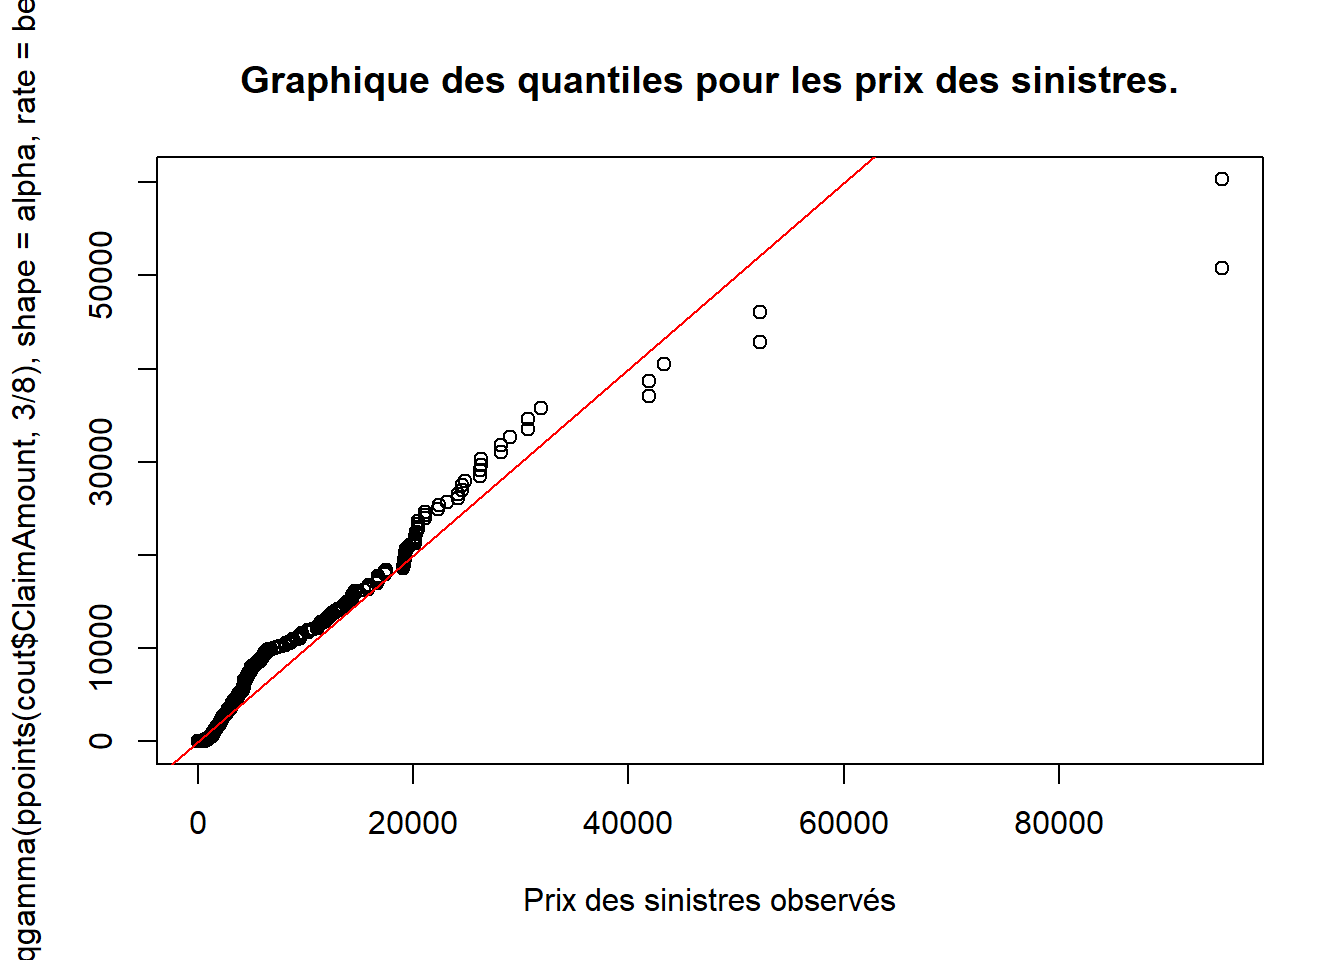
\includegraphics{GLM_sinistralité_Indicatrice_files/figure-latex/unnamed-chunk-4-1.pdf}

La première étape dans la sélection de variables explicatives est
l'étude des corrélations entre ses dernières.

Nous avons déjà fait cette étape dans la première partie donc nous
allons donner directement le modèle.

Nous prendrons dans un premier temps toutes les variables sauf
RecordBeg, RecordEnd, Gender (interdit par la législation française.

Afin de sélectionner au mieux notre modèle, nous devons introduire un
critère de sélection.

Le critère \(AIC\) d'un modèle \([m]\) est

\[
AIC(m)=\frac{n}{2}\log(SCR(m))+m
\]

avec \(SCR(m)=||P_mY-Y||^2\) et \(n\) le nombre d'observations. On
choisit un modèle \([m]\) qui minimise l'\(AIC\). Afin de déterminer le
``meilleur'' modèle pour notre étude, nous utiliserons la méthode
``both''. Cette dernière part de l'intercept et ajoute/enlève les
variables une à une tout en comparant selon le critère \(AIC\).

Nous allons introduire plusieurs modèles. Un modèle vide puis des
modèles pleins utilisant différentes fonctions de lien.

\hypertarget{lien-log}{%
\subsubsection{Lien log}\label{lien-log}}

\begin{Shaded}
\begin{Highlighting}[]
\NormalTok{mod0 }\OtherTok{\textless{}{-}} \FunctionTok{glm}\NormalTok{(ClaimInd }\SpecialCharTok{\textasciitilde{}} \DecValTok{1}\NormalTok{, }\AttributeTok{data =}\NormalTok{ train, }\AttributeTok{family =} \FunctionTok{binomial}\NormalTok{(}\AttributeTok{link =}\NormalTok{ log))}
\FunctionTok{summary}\NormalTok{(mod0)}
\end{Highlighting}
\end{Shaded}

\begin{verbatim}
## 
## Call:
## glm(formula = ClaimInd ~ 1, family = binomial(link = log), data = train)
## 
## Deviance Residuals: 
##     Min       1Q   Median       3Q      Max  
## -0.4406  -0.4406  -0.4406  -0.4406   2.1820  
## 
## Coefficients:
##             Estimate Std. Error z value Pr(>|z|)    
## (Intercept) -2.38052    0.02183  -109.1   <2e-16 ***
## ---
## Signif. codes:  0 '***' 0.001 '**' 0.01 '*' 0.05 '.' 0.1 ' ' 1
## 
## (Dispersion parameter for binomial family taken to be 1)
## 
##     Null deviance: 12698  on 20593  degrees of freedom
## Residual deviance: 12698  on 20593  degrees of freedom
## AIC: 12700
## 
## Number of Fisher Scoring iterations: 6
\end{verbatim}

\begin{Shaded}
\begin{Highlighting}[]
\DecValTok{2}\SpecialCharTok{*}\FunctionTok{as.numeric}\NormalTok{(}\FunctionTok{logLik}\NormalTok{(mod0))}
\end{Highlighting}
\end{Shaded}

\begin{verbatim}
## [1] -12697.86
\end{verbatim}

\begin{Shaded}
\begin{Highlighting}[]
\NormalTok{modFull }\OtherTok{\textless{}{-}} \FunctionTok{glm}\NormalTok{(ClaimInd }\SpecialCharTok{\textasciitilde{}}\NormalTok{ MariStat}\SpecialCharTok{+}\NormalTok{VehUsage}\SpecialCharTok{+}\NormalTok{HasKmLimit}\SpecialCharTok{+}\NormalTok{ClaimNbResp}\SpecialCharTok{+}\NormalTok{ClaimNbNonResp}\SpecialCharTok{+}\NormalTok{ClaimNbParking}\SpecialCharTok{+}\NormalTok{ClaimNbFireTheft}\SpecialCharTok{+}\NormalTok{ClaimNbWindscreen}\SpecialCharTok{+}\NormalTok{OutUseNb}\SpecialCharTok{+}\NormalTok{Risque}\SpecialCharTok{+}\NormalTok{BonusMalus}\SpecialCharTok{+}\NormalTok{DrivAge\_fact}\SpecialCharTok{+}\NormalTok{Categ, }\AttributeTok{data =}\NormalTok{ train, }\AttributeTok{family =} \FunctionTok{binomial}\NormalTok{(}\AttributeTok{link =}\NormalTok{ log))}
\FunctionTok{summary}\NormalTok{(modFull)}
\end{Highlighting}
\end{Shaded}

\begin{verbatim}
## 
## Call:
## glm(formula = ClaimInd ~ MariStat + VehUsage + HasKmLimit + ClaimNbResp + 
##     ClaimNbNonResp + ClaimNbParking + ClaimNbFireTheft + ClaimNbWindscreen + 
##     OutUseNb + Risque + BonusMalus + DrivAge_fact + Categ, family = binomial(link = log), 
##     data = train)
## 
## Deviance Residuals: 
##     Min       1Q   Median       3Q      Max  
## -1.0845  -0.4615  -0.4115  -0.3759   2.4995  
## 
## Coefficients:
##                                 Estimate Std. Error z value Pr(>|z|)    
## (Intercept)                    -3.041823   0.261612 -11.627  < 2e-16 ***
## MariStatOther                   0.025853   0.069465   0.372 0.709761    
## VehUsagePrivate+trip to office  0.068888   0.078427   0.878 0.379741    
## VehUsageProfessional            0.292495   0.091595   3.193 0.001406 ** 
## VehUsageProfessional run        0.299068   0.131674   2.271 0.023130 *  
## HasKmLimit1                    -0.121143   0.097271  -1.245 0.212977    
## ClaimNbResp                     0.103489   0.041178   2.513 0.011963 *  
## ClaimNbNonResp                  0.115937   0.031426   3.689 0.000225 ***
## ClaimNbParking                  0.213293   0.060445   3.529 0.000418 ***
## ClaimNbFireTheft                0.183383   0.063348   2.895 0.003794 ** 
## ClaimNbWindscreen               0.086654   0.029141   2.974 0.002944 ** 
## OutUseNb                        0.040957   0.029864   1.371 0.170226    
## Risque1                        -0.126936   0.121955  -1.041 0.297950    
## Risque2                         0.010606   0.128613   0.082 0.934275    
## Risque3                         0.019807   0.133040   0.149 0.881648    
## Risque4                         0.249555   0.152446   1.637 0.101629    
## BonusMalus                      0.004749   0.001851   2.565 0.010307 *  
## DrivAge_fact(25,30]            -0.082819   0.135297  -0.612 0.540454    
## DrivAge_fact(30,35]            -0.356998   0.139906  -2.552 0.010720 *  
## DrivAge_fact(35,40]            -0.287128   0.142633  -2.013 0.044109 *  
## DrivAge_fact(40,45]            -0.096962   0.143224  -0.677 0.498411    
## DrivAge_fact(45,50]            -0.165780   0.145292  -1.141 0.253863    
## DrivAge_fact(50,58]            -0.278514   0.140869  -1.977 0.048029 *  
## DrivAge_fact(58,65]            -0.139111   0.150916  -0.922 0.356646    
## DrivAge_fact(65,120]           -0.249451   0.166343  -1.500 0.133712    
## Categ1                          0.506362   0.130634   3.876 0.000106 ***
## Categ2                          0.427092   0.149721   2.853 0.004337 ** 
## Categ3                          0.390853   0.121527   3.216 0.001299 ** 
## Categ4                          0.363004   0.155217   2.339 0.019352 *  
## ---
## Signif. codes:  0 '***' 0.001 '**' 0.01 '*' 0.05 '.' 0.1 ' ' 1
## 
## (Dispersion parameter for binomial family taken to be 1)
## 
##     Null deviance: 12698  on 20593  degrees of freedom
## Residual deviance: 12491  on 20565  degrees of freedom
## AIC: 12549
## 
## Number of Fisher Scoring iterations: 6
\end{verbatim}

\begin{Shaded}
\begin{Highlighting}[]
\DecValTok{2}\SpecialCharTok{*}\FunctionTok{as.numeric}\NormalTok{(}\FunctionTok{logLik}\NormalTok{(modFull))}
\end{Highlighting}
\end{Shaded}

\begin{verbatim}
## [1] -12491.46
\end{verbatim}

\begin{Shaded}
\begin{Highlighting}[]
\CommentTok{\#modBoth = step(modFull, mod0, trace=T,direction = c(\textquotesingle{}both\textquotesingle{}))}
\CommentTok{\#summary(modBoth)}
\end{Highlighting}
\end{Shaded}

\begin{Shaded}
\begin{Highlighting}[]
\CommentTok{\#2*as.numeric(logLik(modBoth))}
\end{Highlighting}
\end{Shaded}

Grâce à cette méthode nous obtenons un candidat pour notre modélisation.

\hypertarget{lien-logit-lien-canonique}{%
\subsubsection{Lien logit (lien
canonique)}\label{lien-logit-lien-canonique}}

\begin{Shaded}
\begin{Highlighting}[]
\NormalTok{mod0 }\OtherTok{\textless{}{-}} \FunctionTok{glm}\NormalTok{(ClaimInd }\SpecialCharTok{\textasciitilde{}} \DecValTok{1}\NormalTok{, }\AttributeTok{data =}\NormalTok{ train, }\AttributeTok{family =} \FunctionTok{binomial}\NormalTok{(}\AttributeTok{link =}\NormalTok{ logit))}
\FunctionTok{summary}\NormalTok{(mod0)}
\end{Highlighting}
\end{Shaded}

\begin{verbatim}
## 
## Call:
## glm(formula = ClaimInd ~ 1, family = binomial(link = logit), 
##     data = train)
## 
## Deviance Residuals: 
##     Min       1Q   Median       3Q      Max  
## -0.4406  -0.4406  -0.4406  -0.4406   2.1820  
## 
## Coefficients:
##             Estimate Std. Error z value Pr(>|z|)    
## (Intercept) -2.28345    0.02405  -94.94   <2e-16 ***
## ---
## Signif. codes:  0 '***' 0.001 '**' 0.01 '*' 0.05 '.' 0.1 ' ' 1
## 
## (Dispersion parameter for binomial family taken to be 1)
## 
##     Null deviance: 12698  on 20593  degrees of freedom
## Residual deviance: 12698  on 20593  degrees of freedom
## AIC: 12700
## 
## Number of Fisher Scoring iterations: 5
\end{verbatim}

\begin{Shaded}
\begin{Highlighting}[]
\NormalTok{modFull }\OtherTok{\textless{}{-}} \FunctionTok{glm}\NormalTok{(ClaimInd }\SpecialCharTok{\textasciitilde{}}\NormalTok{ MariStat}\SpecialCharTok{+}\NormalTok{VehUsage}\SpecialCharTok{+}\NormalTok{HasKmLimit}\SpecialCharTok{+}\NormalTok{ClaimNbResp}\SpecialCharTok{+}\NormalTok{ClaimNbNonResp}\SpecialCharTok{+}\NormalTok{ClaimNbParking}\SpecialCharTok{+}\NormalTok{ClaimNbFireTheft}\SpecialCharTok{+}\NormalTok{ClaimNbWindscreen}\SpecialCharTok{+}\NormalTok{OutUseNb}\SpecialCharTok{+}\NormalTok{Risque}\SpecialCharTok{+}\NormalTok{BonusMalus}\SpecialCharTok{+}\NormalTok{Categ}\SpecialCharTok{+}\NormalTok{DrivAge\_fact, }\AttributeTok{data =}\NormalTok{ train, }\AttributeTok{family =} \FunctionTok{binomial}\NormalTok{(}\AttributeTok{link =}\NormalTok{ logit))}
\FunctionTok{summary}\NormalTok{(modFull)}
\end{Highlighting}
\end{Shaded}

\begin{verbatim}
## 
## Call:
## glm(formula = ClaimInd ~ MariStat + VehUsage + HasKmLimit + ClaimNbResp + 
##     ClaimNbNonResp + ClaimNbParking + ClaimNbFireTheft + ClaimNbWindscreen + 
##     OutUseNb + Risque + BonusMalus + Categ + DrivAge_fact, family = binomial(link = logit), 
##     data = train)
## 
## Deviance Residuals: 
##     Min       1Q   Median       3Q      Max  
## -1.0117  -0.4634  -0.4102  -0.3735   2.5183  
## 
## Coefficients:
##                                 Estimate Std. Error z value Pr(>|z|)    
## (Intercept)                    -3.080639   0.295271 -10.433  < 2e-16 ***
## MariStatOther                   0.038152   0.077764   0.491 0.623699    
## VehUsagePrivate+trip to office  0.076346   0.086392   0.884 0.376851    
## VehUsageProfessional            0.335517   0.102044   3.288 0.001009 ** 
## VehUsageProfessional run        0.340185   0.148725   2.287 0.022176 *  
## HasKmLimit1                    -0.125699   0.105371  -1.193 0.232900    
## ClaimNbResp                     0.125942   0.046818   2.690 0.007145 ** 
## ClaimNbNonResp                  0.136365   0.036174   3.770 0.000163 ***
## ClaimNbParking                  0.246198   0.070007   3.517 0.000437 ***
## ClaimNbFireTheft                0.216801   0.074214   2.921 0.003486 ** 
## ClaimNbWindscreen               0.102365   0.033136   3.089 0.002007 ** 
## OutUseNb                        0.049930   0.034046   1.467 0.142499    
## Risque1                        -0.147936   0.135539  -1.091 0.275068    
## Risque2                         0.009096   0.143161   0.064 0.949340    
## Risque3                         0.024434   0.148431   0.165 0.869246    
## Risque4                         0.283316   0.172630   1.641 0.100761    
## BonusMalus                      0.005907   0.002131   2.772 0.005577 ** 
## Categ1                          0.572832   0.144055   3.976 6.99e-05 ***
## Categ2                          0.477981   0.165771   2.883 0.003934 ** 
## Categ3                          0.433797   0.132610   3.271 0.001071 ** 
## Categ4                          0.413109   0.169665   2.435 0.014898 *  
## DrivAge_fact(25,30]            -0.084739   0.155177  -0.546 0.585011    
## DrivAge_fact(30,35]            -0.389282   0.158830  -2.451 0.014249 *  
## DrivAge_fact(35,40]            -0.309196   0.162676  -1.901 0.057344 .  
## DrivAge_fact(40,45]            -0.088170   0.163972  -0.538 0.590776    
## DrivAge_fact(45,50]            -0.174425   0.165911  -1.051 0.293115    
## DrivAge_fact(50,58]            -0.297892   0.160850  -1.852 0.064027 .  
## DrivAge_fact(58,65]            -0.145346   0.172500  -0.843 0.399459    
## DrivAge_fact(65,120]           -0.271711   0.188506  -1.441 0.149473    
## ---
## Signif. codes:  0 '***' 0.001 '**' 0.01 '*' 0.05 '.' 0.1 ' ' 1
## 
## (Dispersion parameter for binomial family taken to be 1)
## 
##     Null deviance: 12698  on 20593  degrees of freedom
## Residual deviance: 12487  on 20565  degrees of freedom
## AIC: 12545
## 
## Number of Fisher Scoring iterations: 5
\end{verbatim}

\begin{Shaded}
\begin{Highlighting}[]
\DecValTok{2}\SpecialCharTok{*}\FunctionTok{as.numeric}\NormalTok{(}\FunctionTok{logLik}\NormalTok{(modFull))}
\end{Highlighting}
\end{Shaded}

\begin{verbatim}
## [1] -12486.54
\end{verbatim}

\begin{Shaded}
\begin{Highlighting}[]
\NormalTok{modBoth\_Bin }\OtherTok{\textless{}{-}} \FunctionTok{step}\NormalTok{(modFull, mod0, }\AttributeTok{trace =}\NormalTok{ F, }\AttributeTok{direction =} \FunctionTok{c}\NormalTok{(}\StringTok{\textquotesingle{}both\textquotesingle{}}\NormalTok{))}
\FunctionTok{summary}\NormalTok{(modBoth\_Bin)}
\end{Highlighting}
\end{Shaded}

\begin{verbatim}
## 
## Call:
## glm(formula = ClaimInd ~ VehUsage + ClaimNbResp + ClaimNbNonResp + 
##     ClaimNbParking + ClaimNbFireTheft + ClaimNbWindscreen + OutUseNb + 
##     Risque + BonusMalus + Categ + DrivAge_fact, family = binomial(link = logit), 
##     data = train)
## 
## Deviance Residuals: 
##     Min       1Q   Median       3Q      Max  
## -1.0084  -0.4633  -0.4107  -0.3714   2.5233  
## 
## Coefficients:
##                                  Estimate Std. Error z value Pr(>|z|)    
## (Intercept)                    -3.0679872  0.2915474 -10.523  < 2e-16 ***
## VehUsagePrivate+trip to office  0.0827724  0.0860324   0.962 0.335996    
## VehUsageProfessional            0.3488673  0.1014583   3.439 0.000585 ***
## VehUsageProfessional run        0.3525928  0.1483510   2.377 0.017466 *  
## ClaimNbResp                     0.1270307  0.0468009   2.714 0.006642 ** 
## ClaimNbNonResp                  0.1379437  0.0361493   3.816 0.000136 ***
## ClaimNbParking                  0.2477350  0.0699214   3.543 0.000396 ***
## ClaimNbFireTheft                0.2175395  0.0741668   2.933 0.003356 ** 
## ClaimNbWindscreen               0.1049567  0.0330735   3.173 0.001506 ** 
## OutUseNb                        0.0503704  0.0340347   1.480 0.138881    
## Risque1                        -0.1527232  0.1354696  -1.127 0.259590    
## Risque2                         0.0003875  0.1430107   0.003 0.997838    
## Risque3                         0.0143903  0.1482378   0.097 0.922666    
## Risque4                         0.2828270  0.1726019   1.639 0.101295    
## BonusMalus                      0.0057997  0.0021225   2.732 0.006287 ** 
## Categ1                          0.5766523  0.1440473   4.003 6.25e-05 ***
## Categ2                          0.4815675  0.1657402   2.906 0.003666 ** 
## Categ3                          0.4350687  0.1325996   3.281 0.001034 ** 
## Categ4                          0.4141763  0.1696861   2.441 0.014653 *  
## DrivAge_fact(25,30]            -0.0759519  0.1542147  -0.493 0.622360    
## DrivAge_fact(30,35]            -0.3765928  0.1559318  -2.415 0.015730 *  
## DrivAge_fact(35,40]            -0.2932346  0.1590734  -1.843 0.065272 .  
## DrivAge_fact(40,45]            -0.0733110  0.1599877  -0.458 0.646788    
## DrivAge_fact(45,50]            -0.1589061  0.1619034  -0.981 0.326353    
## DrivAge_fact(50,58]            -0.2807162  0.1561678  -1.798 0.072252 .  
## DrivAge_fact(58,65]            -0.1282297  0.1679287  -0.764 0.445108    
## DrivAge_fact(65,120]           -0.2608048  0.1841688  -1.416 0.156741    
## ---
## Signif. codes:  0 '***' 0.001 '**' 0.01 '*' 0.05 '.' 0.1 ' ' 1
## 
## (Dispersion parameter for binomial family taken to be 1)
## 
##     Null deviance: 12698  on 20593  degrees of freedom
## Residual deviance: 12488  on 20567  degrees of freedom
## AIC: 12542
## 
## Number of Fisher Scoring iterations: 5
\end{verbatim}

\hypertarget{lien-probit}{%
\subsubsection{Lien probit}\label{lien-probit}}

\begin{Shaded}
\begin{Highlighting}[]
\NormalTok{mod0 }\OtherTok{\textless{}{-}} \FunctionTok{glm}\NormalTok{(ClaimInd }\SpecialCharTok{\textasciitilde{}} \DecValTok{1}\NormalTok{, }\AttributeTok{data =}\NormalTok{ train, }\AttributeTok{family =} \FunctionTok{binomial}\NormalTok{(}\AttributeTok{link =} \StringTok{"probit"}\NormalTok{))}
\FunctionTok{summary}\NormalTok{(mod0)}
\end{Highlighting}
\end{Shaded}

\begin{verbatim}
## 
## Call:
## glm(formula = ClaimInd ~ 1, family = binomial(link = "probit"), 
##     data = train)
## 
## Deviance Residuals: 
##     Min       1Q   Median       3Q      Max  
## -0.4406  -0.4406  -0.4406  -0.4406   2.1820  
## 
## Coefficients:
##             Estimate Std. Error z value Pr(>|z|)    
## (Intercept) -1.32550    0.01218  -108.8   <2e-16 ***
## ---
## Signif. codes:  0 '***' 0.001 '**' 0.01 '*' 0.05 '.' 0.1 ' ' 1
## 
## (Dispersion parameter for binomial family taken to be 1)
## 
##     Null deviance: 12698  on 20593  degrees of freedom
## Residual deviance: 12698  on 20593  degrees of freedom
## AIC: 12700
## 
## Number of Fisher Scoring iterations: 4
\end{verbatim}

\begin{Shaded}
\begin{Highlighting}[]
\NormalTok{modFull }\OtherTok{\textless{}{-}} \FunctionTok{glm}\NormalTok{(ClaimInd }\SpecialCharTok{\textasciitilde{}}\NormalTok{ MariStat}\SpecialCharTok{+}\NormalTok{Categ}\SpecialCharTok{+}\NormalTok{VehUsage}\SpecialCharTok{+}\NormalTok{HasKmLimit}\SpecialCharTok{+}\NormalTok{ClaimNbResp}\SpecialCharTok{+}\NormalTok{ClaimNbNonResp}\SpecialCharTok{+}\NormalTok{ClaimNbParking}\SpecialCharTok{+}\NormalTok{ClaimNbFireTheft}\SpecialCharTok{+}\NormalTok{ClaimNbWindscreen}\SpecialCharTok{+}\NormalTok{OutUseNb}\SpecialCharTok{+}\NormalTok{Risque}\SpecialCharTok{+}\NormalTok{BonusMalus}\SpecialCharTok{+}\NormalTok{DrivAge\_fact, }\AttributeTok{data =}\NormalTok{ train, }\AttributeTok{family =} \FunctionTok{binomial}\NormalTok{(}\AttributeTok{link =}\NormalTok{ probit))}
\FunctionTok{summary}\NormalTok{(modFull)}
\end{Highlighting}
\end{Shaded}

\begin{verbatim}
## 
## Call:
## glm(formula = ClaimInd ~ MariStat + Categ + VehUsage + HasKmLimit + 
##     ClaimNbResp + ClaimNbNonResp + ClaimNbParking + ClaimNbFireTheft + 
##     ClaimNbWindscreen + OutUseNb + Risque + BonusMalus + DrivAge_fact, 
##     family = binomial(link = probit), data = train)
## 
## Deviance Residuals: 
##     Min       1Q   Median       3Q      Max  
## -0.9614  -0.4654  -0.4103  -0.3703   2.5422  
## 
## Coefficients:
##                                 Estimate Std. Error z value Pr(>|z|)    
## (Intercept)                    -1.744661   0.151958 -11.481  < 2e-16 ***
## MariStatOther                   0.025889   0.039770   0.651 0.515066    
## Categ1                          0.291767   0.072230   4.039 5.36e-05 ***
## Categ2                          0.241425   0.083675   2.885 0.003911 ** 
## Categ3                          0.216764   0.065299   3.320 0.000902 ***
## Categ4                          0.212360   0.083732   2.536 0.011207 *  
## VehUsagePrivate+trip to office  0.038547   0.043324   0.890 0.373598    
## VehUsageProfessional            0.175106   0.051992   3.368 0.000757 ***
## VehUsageProfessional run        0.178097   0.077157   2.308 0.020985 *  
## HasKmLimit1                    -0.060040   0.051523  -1.165 0.243892    
## ClaimNbResp                     0.067900   0.024402   2.783 0.005392 ** 
## ClaimNbNonResp                  0.073124   0.019046   3.839 0.000123 ***
## ClaimNbParking                  0.130858   0.037189   3.519 0.000434 ***
## ClaimNbFireTheft                0.111993   0.039358   2.845 0.004434 ** 
## ClaimNbWindscreen               0.053928   0.017265   3.124 0.001787 ** 
## OutUseNb                        0.027793   0.017864   1.556 0.119764    
## Risque1                        -0.080681   0.068833  -1.172 0.241147    
## Risque2                         0.002668   0.072873   0.037 0.970791    
## Risque3                         0.012081   0.075763   0.159 0.873305    
## Risque4                         0.145105   0.089660   1.618 0.105578    
## BonusMalus                      0.003196   0.001122   2.848 0.004402 ** 
## DrivAge_fact(25,30]            -0.041150   0.082036  -0.502 0.615940    
## DrivAge_fact(30,35]            -0.196091   0.082896  -2.366 0.018005 *  
## DrivAge_fact(35,40]            -0.155372   0.085234  -1.823 0.068320 .  
## DrivAge_fact(40,45]            -0.039192   0.086320  -0.454 0.649804    
## DrivAge_fact(45,50]            -0.088093   0.087099  -1.011 0.311820    
## DrivAge_fact(50,58]            -0.150325   0.084396  -1.781 0.074883 .  
## DrivAge_fact(58,65]            -0.076890   0.090482  -0.850 0.395446    
## DrivAge_fact(65,120]           -0.140629   0.097872  -1.437 0.150755    
## ---
## Signif. codes:  0 '***' 0.001 '**' 0.01 '*' 0.05 '.' 0.1 ' ' 1
## 
## (Dispersion parameter for binomial family taken to be 1)
## 
##     Null deviance: 12698  on 20593  degrees of freedom
## Residual deviance: 12482  on 20565  degrees of freedom
## AIC: 12540
## 
## Number of Fisher Scoring iterations: 5
\end{verbatim}

\begin{Shaded}
\begin{Highlighting}[]
\DecValTok{2}\SpecialCharTok{*}\FunctionTok{as.numeric}\NormalTok{(}\FunctionTok{logLik}\NormalTok{(modFull))}
\end{Highlighting}
\end{Shaded}

\begin{verbatim}
## [1] -12482.47
\end{verbatim}

\hypertarget{lien-cauchit}{%
\subsubsection{Lien cauchit}\label{lien-cauchit}}

\begin{Shaded}
\begin{Highlighting}[]
\NormalTok{modFull }\OtherTok{\textless{}{-}} \FunctionTok{glm}\NormalTok{(ClaimInd }\SpecialCharTok{\textasciitilde{}}\NormalTok{ MariStat}\SpecialCharTok{+}\NormalTok{Categ}\SpecialCharTok{+}\NormalTok{VehUsage}\SpecialCharTok{+}\NormalTok{HasKmLimit}\SpecialCharTok{+}\NormalTok{ClaimNbResp}\SpecialCharTok{+}\NormalTok{ClaimNbNonResp}\SpecialCharTok{+}\NormalTok{ClaimNbParking}\SpecialCharTok{+}\NormalTok{ClaimNbFireTheft}\SpecialCharTok{+}\NormalTok{ClaimNbWindscreen}\SpecialCharTok{+}\NormalTok{OutUseNb}\SpecialCharTok{+}\NormalTok{Risque}\SpecialCharTok{+}\NormalTok{BonusMalus}\SpecialCharTok{+}\NormalTok{DrivAge\_fact, }\AttributeTok{data =}\NormalTok{ train, }\AttributeTok{family =} \FunctionTok{binomial}\NormalTok{(}\AttributeTok{link =}\NormalTok{ cauchit))}
\FunctionTok{summary}\NormalTok{(modFull)}
\end{Highlighting}
\end{Shaded}

\begin{verbatim}
## 
## Call:
## glm(formula = ClaimInd ~ MariStat + Categ + VehUsage + HasKmLimit + 
##     ClaimNbResp + ClaimNbNonResp + ClaimNbParking + ClaimNbFireTheft + 
##     ClaimNbWindscreen + OutUseNb + Risque + BonusMalus + DrivAge_fact, 
##     family = binomial(link = cauchit), data = train)
## 
## Deviance Residuals: 
##     Min       1Q   Median       3Q      Max  
## -1.3318  -0.4554  -0.4181  -0.3930   2.3940  
## 
## Coefficients:
##                                 Estimate Std. Error z value Pr(>|z|)    
## (Intercept)                    -4.857679   0.851992  -5.702 1.19e-08 ***
## MariStatOther                  -0.049809   0.212514  -0.234 0.814690    
## Categ1                          1.623133   0.509489   3.186 0.001444 ** 
## Categ2                          1.383714   0.557482   2.482 0.013062 *  
## Categ3                          1.329074   0.496868   2.675 0.007475 ** 
## Categ4                          1.034885   0.612083   1.691 0.090883 .  
## VehUsagePrivate+trip to office  0.223494   0.277896   0.804 0.421260    
## VehUsageProfessional            0.797407   0.303944   2.624 0.008702 ** 
## VehUsageProfessional run        0.781515   0.403163   1.938 0.052567 .  
## HasKmLimit1                    -0.642163   0.421707  -1.523 0.127817    
## ClaimNbResp                     0.192678   0.118854   1.621 0.104990    
## ClaimNbNonResp                  0.243804   0.084991   2.869 0.004123 ** 
## ClaimNbParking                  0.549101   0.149665   3.669 0.000244 ***
## ClaimNbFireTheft                0.459150   0.156551   2.933 0.003358 ** 
## ClaimNbWindscreen               0.205287   0.083728   2.452 0.014213 *  
## OutUseNb                        0.081598   0.084929   0.961 0.336666    
## Risque1                        -0.280252   0.406373  -0.690 0.490420    
## Risque2                         0.101320   0.422964   0.240 0.810682    
## Risque3                         0.041356   0.433057   0.095 0.923919    
## Risque4                         0.716289   0.459466   1.559 0.119005    
## BonusMalus                      0.008837   0.005249   1.684 0.092271 .  
## DrivAge_fact(25,30]            -0.380944   0.349628  -1.090 0.275902    
## DrivAge_fact(30,35]            -1.234253   0.406539  -3.036 0.002397 ** 
## DrivAge_fact(35,40]            -1.007741   0.395074  -2.551 0.010749 *  
## DrivAge_fact(40,45]            -0.508037   0.383407  -1.325 0.185152    
## DrivAge_fact(45,50]            -0.606073   0.395143  -1.534 0.125077    
## DrivAge_fact(50,58]            -0.981487   0.387096  -2.536 0.011228 *  
## DrivAge_fact(58,65]            -0.513208   0.410694  -1.250 0.211442    
## DrivAge_fact(65,120]           -0.774640   0.487503  -1.589 0.112061    
## ---
## Signif. codes:  0 '***' 0.001 '**' 0.01 '*' 0.05 '.' 0.1 ' ' 1
## 
## (Dispersion parameter for binomial family taken to be 1)
## 
##     Null deviance: 12698  on 20593  degrees of freedom
## Residual deviance: 12524  on 20565  degrees of freedom
## AIC: 12582
## 
## Number of Fisher Scoring iterations: 7
\end{verbatim}

\begin{Shaded}
\begin{Highlighting}[]
\DecValTok{2}\SpecialCharTok{*}\FunctionTok{as.numeric}\NormalTok{(}\FunctionTok{logLik}\NormalTok{(modFull))}
\end{Highlighting}
\end{Shaded}

\begin{verbatim}
## [1] -12523.9
\end{verbatim}

\hypertarget{lien-cloglog}{%
\subsubsection{Lien cloglog}\label{lien-cloglog}}

\begin{Shaded}
\begin{Highlighting}[]
\NormalTok{modFull }\OtherTok{\textless{}{-}} \FunctionTok{glm}\NormalTok{(ClaimInd }\SpecialCharTok{\textasciitilde{}}\NormalTok{ MariStat}\SpecialCharTok{+}\NormalTok{Categ}\SpecialCharTok{+}\NormalTok{VehUsage}\SpecialCharTok{+}\NormalTok{HasKmLimit}\SpecialCharTok{+}\NormalTok{ClaimNbResp}\SpecialCharTok{+}\NormalTok{ClaimNbNonResp}\SpecialCharTok{+}\NormalTok{ClaimNbParking}\SpecialCharTok{+}\NormalTok{ClaimNbFireTheft}\SpecialCharTok{+}\NormalTok{ClaimNbWindscreen}\SpecialCharTok{+}\NormalTok{OutUseNb}\SpecialCharTok{+}\NormalTok{Risque}\SpecialCharTok{+}\NormalTok{BonusMalus}\SpecialCharTok{+}\NormalTok{DrivAge\_fact, }\AttributeTok{data =}\NormalTok{ train, }\AttributeTok{family =} \FunctionTok{binomial}\NormalTok{(}\AttributeTok{link =}\NormalTok{ cloglog))}
\FunctionTok{summary}\NormalTok{(modFull)}
\end{Highlighting}
\end{Shaded}

\begin{verbatim}
## 
## Call:
## glm(formula = ClaimInd ~ MariStat + Categ + VehUsage + HasKmLimit + 
##     ClaimNbResp + ClaimNbNonResp + ClaimNbParking + ClaimNbFireTheft + 
##     ClaimNbWindscreen + OutUseNb + Risque + BonusMalus + DrivAge_fact, 
##     family = binomial(link = cloglog), data = train)
## 
## Deviance Residuals: 
##     Min       1Q   Median       3Q      Max  
## -1.0466  -0.4624  -0.4108  -0.3743   2.5093  
## 
## Coefficients:
##                                 Estimate Std. Error z value Pr(>|z|)    
## (Intercept)                    -3.063775   0.278218 -11.012  < 2e-16 ***
## MariStatOther                   0.031902   0.073560   0.434 0.664515    
## Categ1                          0.539587   0.137208   3.933  8.4e-05 ***
## Categ2                          0.452369   0.157592   2.871 0.004098 ** 
## Categ3                          0.412321   0.126981   3.247 0.001166 ** 
## Categ4                          0.387931   0.162341   2.390 0.016867 *  
## VehUsagePrivate+trip to office  0.072616   0.082353   0.882 0.377902    
## VehUsageProfessional            0.313901   0.096730   3.245 0.001174 ** 
## VehUsageProfessional run        0.319224   0.140032   2.280 0.022628 *  
## HasKmLimit1                    -0.123251   0.101257  -1.217 0.223521    
## ClaimNbResp                     0.114794   0.043953   2.612 0.009008 ** 
## ClaimNbNonResp                  0.126052   0.033770   3.733 0.000189 ***
## ClaimNbParking                  0.229450   0.065155   3.522 0.000429 ***
## ClaimNbFireTheft                0.201252   0.068833   2.924 0.003458 ** 
## ClaimNbWindscreen               0.094549   0.031106   3.040 0.002369 ** 
## OutUseNb                        0.045338   0.031911   1.421 0.155377    
## Risque1                        -0.137081   0.128645  -1.066 0.286616    
## Risque2                         0.009910   0.135776   0.073 0.941814    
## Risque3                         0.022385   0.140615   0.159 0.873515    
## Risque4                         0.266926   0.162376   1.644 0.100202    
## BonusMalus                      0.005344   0.001989   2.687 0.007216 ** 
## DrivAge_fact(25,30]            -0.083411   0.145059  -0.575 0.565282    
## DrivAge_fact(30,35]            -0.372564   0.149196  -2.497 0.012520 *  
## DrivAge_fact(35,40]            -0.297243   0.152487  -1.949 0.051260 .  
## DrivAge_fact(40,45]            -0.091831   0.153424  -0.599 0.549479    
## DrivAge_fact(45,50]            -0.169252   0.155427  -1.089 0.276178    
## DrivAge_fact(50,58]            -0.287282   0.150690  -1.906 0.056594 .  
## DrivAge_fact(58,65]            -0.140828   0.161556  -0.872 0.383373    
## DrivAge_fact(65,120]           -0.259446   0.177254  -1.464 0.143277    
## ---
## Signif. codes:  0 '***' 0.001 '**' 0.01 '*' 0.05 '.' 0.1 ' ' 1
## 
## (Dispersion parameter for binomial family taken to be 1)
## 
##     Null deviance: 12698  on 20593  degrees of freedom
## Residual deviance: 12489  on 20565  degrees of freedom
## AIC: 12547
## 
## Number of Fisher Scoring iterations: 5
\end{verbatim}

\begin{Shaded}
\begin{Highlighting}[]
\DecValTok{2}\SpecialCharTok{*}\FunctionTok{as.numeric}\NormalTok{(}\FunctionTok{logLik}\NormalTok{(modFull))}
\end{Highlighting}
\end{Shaded}

\begin{verbatim}
## [1] -12488.8
\end{verbatim}

\hypertarget{etude-de-potentiels-outliers}{%
\subsection{Etude de potentiels
outliers}\label{etude-de-potentiels-outliers}}

Un élément important à prendre en compte dans l'analyse des données est
le traitement des outliers. Voyons si nous observons des candidats
potentiels par lecture graphique

\begin{Shaded}
\begin{Highlighting}[]
\NormalTok{modFull }\OtherTok{\textless{}{-}} \FunctionTok{glm}\NormalTok{(ClaimInd }\SpecialCharTok{\textasciitilde{}}\NormalTok{ MariStat}\SpecialCharTok{+}\NormalTok{VehUsage}\SpecialCharTok{+}\NormalTok{HasKmLimit}\SpecialCharTok{+}\NormalTok{ClaimNbResp}\SpecialCharTok{+}\NormalTok{ClaimNbNonResp}\SpecialCharTok{+}\NormalTok{ClaimNbParking}\SpecialCharTok{+}\NormalTok{ClaimNbFireTheft}\SpecialCharTok{+}\NormalTok{ClaimNbWindscreen}\SpecialCharTok{+}\NormalTok{OutUseNb}\SpecialCharTok{+}\NormalTok{Risque}\SpecialCharTok{+}\NormalTok{BonusMalus}\SpecialCharTok{+}\NormalTok{Categ}\SpecialCharTok{+}\NormalTok{DrivAge\_fact, }\AttributeTok{data =}\NormalTok{ train, }\AttributeTok{family =} \FunctionTok{binomial}\NormalTok{(}\AttributeTok{link =}\NormalTok{ logit))}
\FunctionTok{plot}\NormalTok{(modFull)}
\end{Highlighting}
\end{Shaded}

\includegraphics{GLM_sinistralité_Indicatrice_files/figure-latex/unnamed-chunk-22-1.pdf}
\includegraphics{GLM_sinistralité_Indicatrice_files/figure-latex/unnamed-chunk-22-2.pdf}
\includegraphics{GLM_sinistralité_Indicatrice_files/figure-latex/unnamed-chunk-22-3.pdf}
\includegraphics{GLM_sinistralité_Indicatrice_files/figure-latex/unnamed-chunk-22-4.pdf}

Test pour voir si il y a des outliers :

\begin{Shaded}
\begin{Highlighting}[]
\FunctionTok{influenceIndexPlot}\NormalTok{(modFull)}
\end{Highlighting}
\end{Shaded}

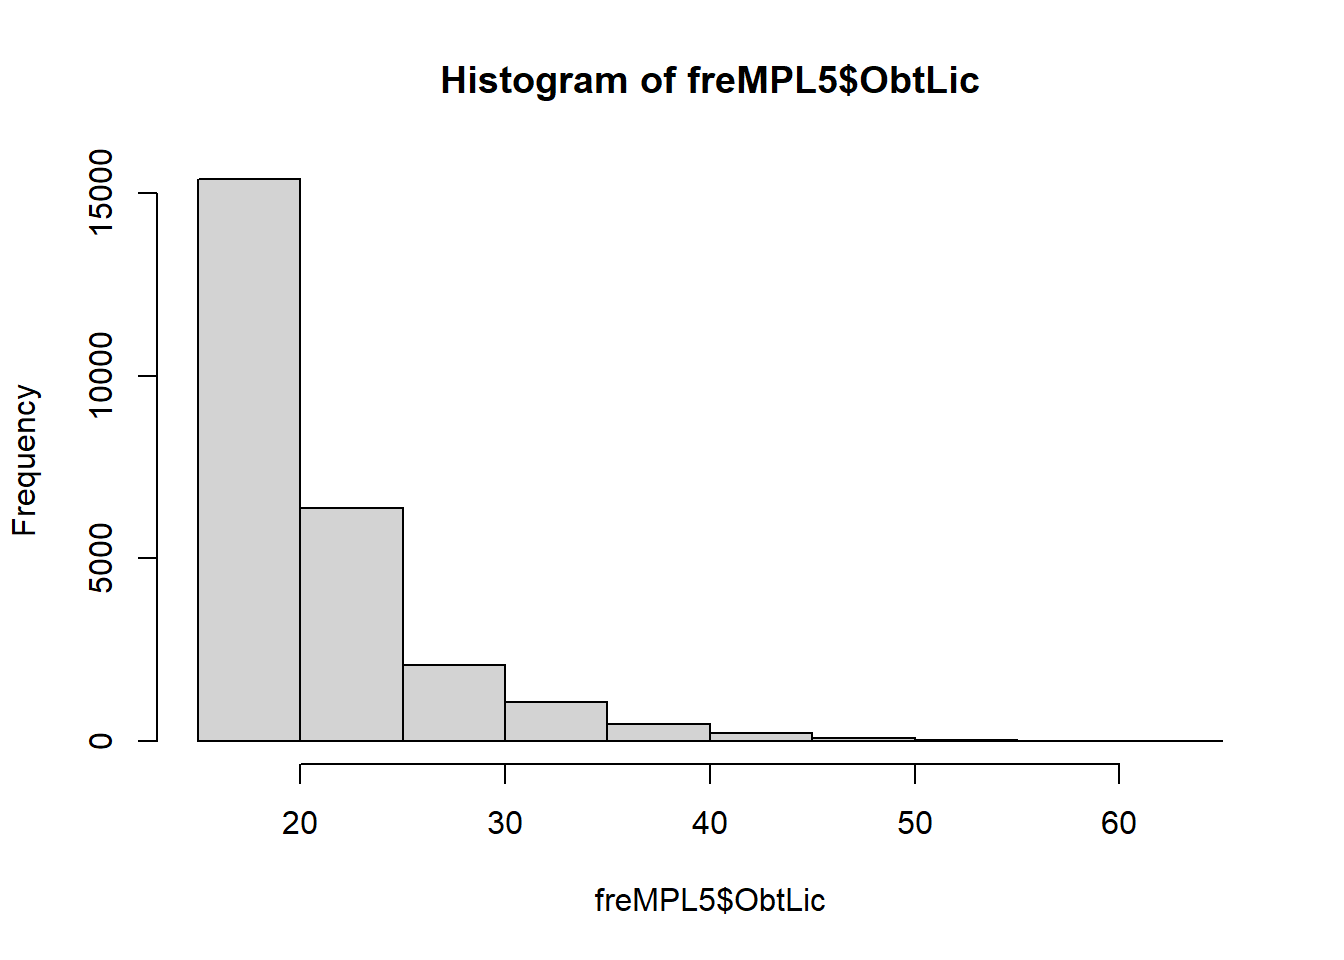
\includegraphics{GLM_sinistralité_Indicatrice_files/figure-latex/unnamed-chunk-23-1.pdf}

\begin{Shaded}
\begin{Highlighting}[]
\FunctionTok{outlierTest}\NormalTok{(modFull)}
\end{Highlighting}
\end{Shaded}

\begin{verbatim}
## No Studentized residuals with Bonferroni p < 0.05
## Largest |rstudent|:
##      rstudent unadjusted p-value Bonferroni p
## 9014 2.522865            0.01164           NA
\end{verbatim}

Si p-Bonferroni \textgreater0,05 alors on conserve l'hyptohèse que ce
n'est pas un outlier.

Il n'y a donc pas d'outlier ici dans ce modèle.

\hypertarget{pruxe9diction-avec-le-moduxe8le-binomial}{%
\subsection{Prédiction avec le modèle
binomial}\label{pruxe9diction-avec-le-moduxe8le-binomial}}

\hypertarget{evaluation-du-moduxe8le-sur-les-donnuxe9es-tests}{%
\subsubsection{Evaluation du modèle sur les données
tests}\label{evaluation-du-moduxe8le-sur-les-donnuxe9es-tests}}

\begin{Shaded}
\begin{Highlighting}[]
\NormalTok{estimation }\OtherTok{\textless{}{-}}\NormalTok{ modFull}\SpecialCharTok{$}\NormalTok{fitted.values}
\FunctionTok{hist}\NormalTok{(estimation)}
\end{Highlighting}
\end{Shaded}

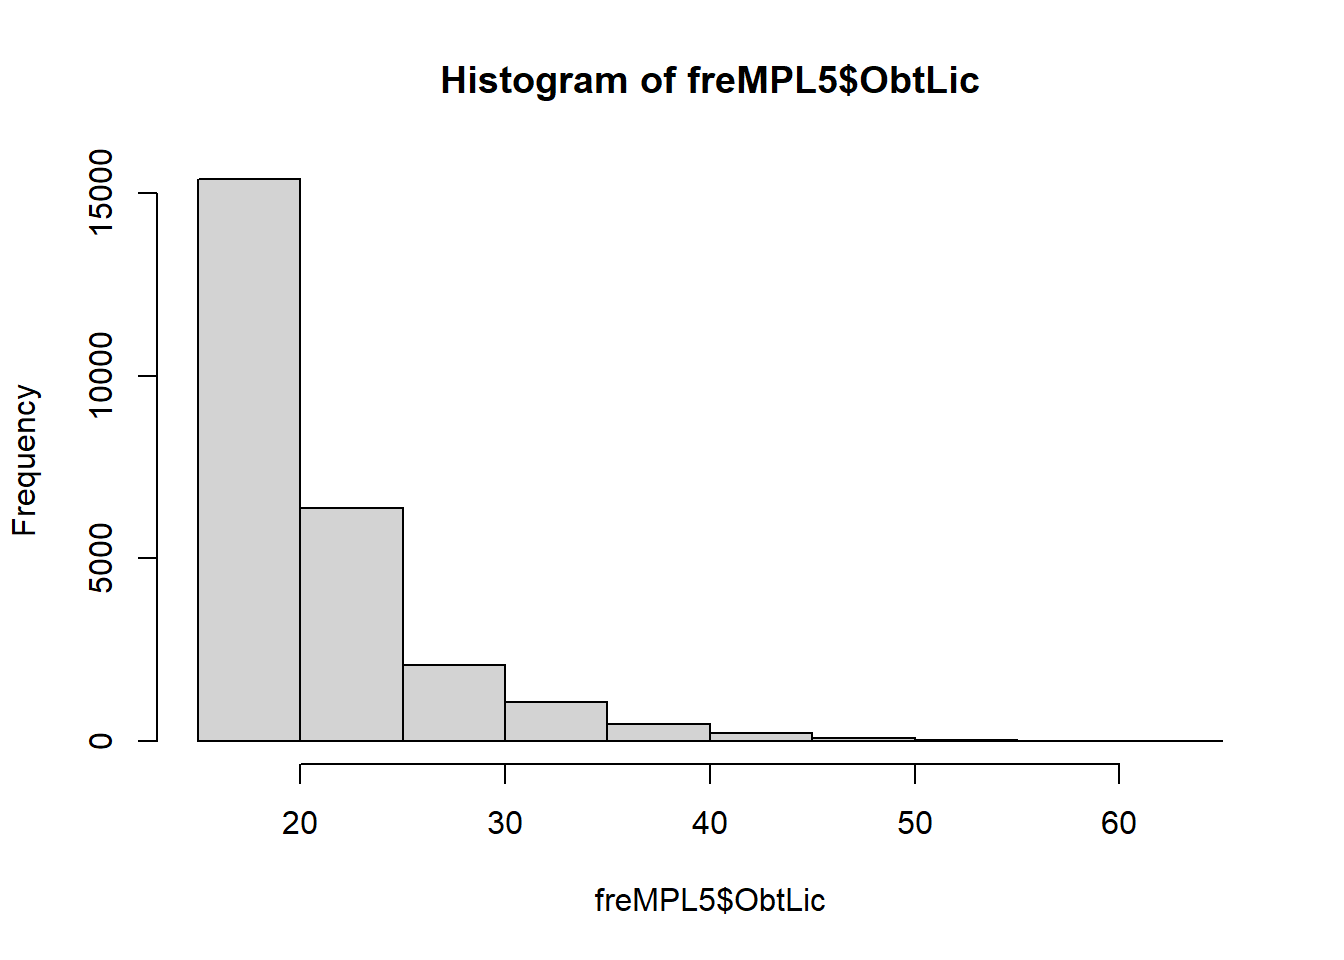
\includegraphics{GLM_sinistralité_Indicatrice_files/figure-latex/unnamed-chunk-24-1.pdf}

\hypertarget{utilisation-de-muxe9triques-de-comparaison}{%
\subsubsection{Utilisation de métriques de
comparaison}\label{utilisation-de-muxe9triques-de-comparaison}}

\hypertarget{rmse}{%
\paragraph{RMSE}\label{rmse}}

\begin{Shaded}
\begin{Highlighting}[]
\NormalTok{pred}\OtherTok{=}\FunctionTok{predict.glm}\NormalTok{(modFull, }\AttributeTok{newdata =}\NormalTok{ test, }\AttributeTok{type =} \StringTok{"response"}\NormalTok{)}
\NormalTok{RMSE\_test }\OtherTok{\textless{}{-}} \FunctionTok{sqrt}\NormalTok{(}\FunctionTok{mean}\NormalTok{((pred }\SpecialCharTok{{-}}\NormalTok{ test}\SpecialCharTok{$}\NormalTok{ClaimInd)}\SpecialCharTok{\^{}}\DecValTok{2}\NormalTok{))}
\NormalTok{RMSE\_test}
\end{Highlighting}
\end{Shaded}

\begin{verbatim}
## [1] 0.2999176
\end{verbatim}

\hypertarget{auc}{%
\subsubsection{AUC}\label{auc}}

\hypertarget{sur-le-jeu-de-donnuxe9es-train}{%
\paragraph{Sur le jeu de données
train}\label{sur-le-jeu-de-donnuxe9es-train}}

\begin{Shaded}
\begin{Highlighting}[]
\NormalTok{pred}\OtherTok{=}\FunctionTok{prediction}\NormalTok{(modFull}\SpecialCharTok{$}\NormalTok{fitted.values, train}\SpecialCharTok{$}\NormalTok{ClaimInd)}
\NormalTok{perf}\OtherTok{=}\FunctionTok{performance}\NormalTok{(pred,}\StringTok{"tpr"}\NormalTok{, }\StringTok{"fpr"}\NormalTok{)}

\NormalTok{auc\_ROCR }\OtherTok{\textless{}{-}} \FunctionTok{performance}\NormalTok{(pred, }\AttributeTok{measure =} \StringTok{"auc"}\NormalTok{)}
\NormalTok{(auc\_ROCR }\OtherTok{\textless{}{-}} \FunctionTok{round}\NormalTok{(auc\_ROCR}\SpecialCharTok{@}\NormalTok{y.values[[}\DecValTok{1}\NormalTok{]],}\DecValTok{3}\NormalTok{) )}
\end{Highlighting}
\end{Shaded}

\begin{verbatim}
## [1] 0.604
\end{verbatim}

\hypertarget{sur-le-jeu-de-donnuxe9es-test}{%
\paragraph{Sur le jeu de données
test}\label{sur-le-jeu-de-donnuxe9es-test}}

\begin{Shaded}
\begin{Highlighting}[]
\NormalTok{prev\_step }\OtherTok{\textless{}{-}} \FunctionTok{predict}\NormalTok{(modFull,}\AttributeTok{newdata=}\NormalTok{test,}\AttributeTok{type=}\StringTok{"response"}\NormalTok{)}
\NormalTok{prev\_prob }\OtherTok{\textless{}{-}} \FunctionTok{data.frame}\NormalTok{(}\AttributeTok{complet=}\FunctionTok{predict}\NormalTok{(modFull,}\AttributeTok{newdata=}\NormalTok{test, }\AttributeTok{type=}\StringTok{"response"}\NormalTok{),}\AttributeTok{vide=}\FunctionTok{predict}\NormalTok{(mod0,}\AttributeTok{newdata=}\NormalTok{test,}\AttributeTok{type=}\StringTok{"response"}\NormalTok{))}
\FunctionTok{head}\NormalTok{(}\FunctionTok{round}\NormalTok{(prev\_prob,}\DecValTok{3}\NormalTok{), }\AttributeTok{n=}\DecValTok{3}\NormalTok{)}
\end{Highlighting}
\end{Shaded}

\begin{verbatim}
##    complet  vide
## 5    0.058 0.093
## 11   0.070 0.093
## 17   0.090 0.093
\end{verbatim}

\begin{Shaded}
\begin{Highlighting}[]
\NormalTok{prev\_class }\OtherTok{\textless{}{-}} \FunctionTok{ifelse}\NormalTok{(prev\_prob}\SpecialCharTok{\textgreater{}}\FloatTok{0.2}\NormalTok{, }\DecValTok{1}\NormalTok{, }\DecValTok{0}\NormalTok{)}
\FunctionTok{head}\NormalTok{(prev\_class, }\AttributeTok{n=}\DecValTok{3}\NormalTok{)}
\end{Highlighting}
\end{Shaded}

\begin{verbatim}
##    complet vide
## 5        0    0
## 11       0    0
## 17       0    0
\end{verbatim}

\begin{Shaded}
\begin{Highlighting}[]
\FunctionTok{mean}\NormalTok{(}\FunctionTok{as.factor}\NormalTok{(prev\_class[,}\DecValTok{1}\NormalTok{])}\SpecialCharTok{==}\NormalTok{test}\SpecialCharTok{$}\NormalTok{ClaimInd)}
\end{Highlighting}
\end{Shaded}

\begin{verbatim}
## [1] 0.8954758
\end{verbatim}

\begin{Shaded}
\begin{Highlighting}[]
\FunctionTok{mean}\NormalTok{(}\FunctionTok{as.factor}\NormalTok{(prev\_class[,}\DecValTok{2}\NormalTok{])}\SpecialCharTok{==}\NormalTok{test}\SpecialCharTok{$}\NormalTok{ClaimInd)}
\end{Highlighting}
\end{Shaded}

\begin{verbatim}
## [1] 0.899961
\end{verbatim}

\begin{Shaded}
\begin{Highlighting}[]
\NormalTok{df\_roc }\OtherTok{\textless{}{-}}\NormalTok{ prev\_prob }\SpecialCharTok{\%\textgreater{}\%} \FunctionTok{mutate}\NormalTok{(}\AttributeTok{obs=}\FunctionTok{as.numeric}\NormalTok{(test}\SpecialCharTok{$}\NormalTok{ClaimInd)) }\SpecialCharTok{\%\textgreater{}\%} \FunctionTok{gather}\NormalTok{(}\AttributeTok{key=}\NormalTok{methode,}\AttributeTok{value=}\NormalTok{score,complet,vide)}
\FunctionTok{ggplot}\NormalTok{(df\_roc, }\FunctionTok{aes}\NormalTok{(}\AttributeTok{m=}\NormalTok{score, }\AttributeTok{d=}\NormalTok{obs,}\AttributeTok{color=}\NormalTok{methode))}\SpecialCharTok{+} \FunctionTok{geom\_roc}\NormalTok{()}
\end{Highlighting}
\end{Shaded}

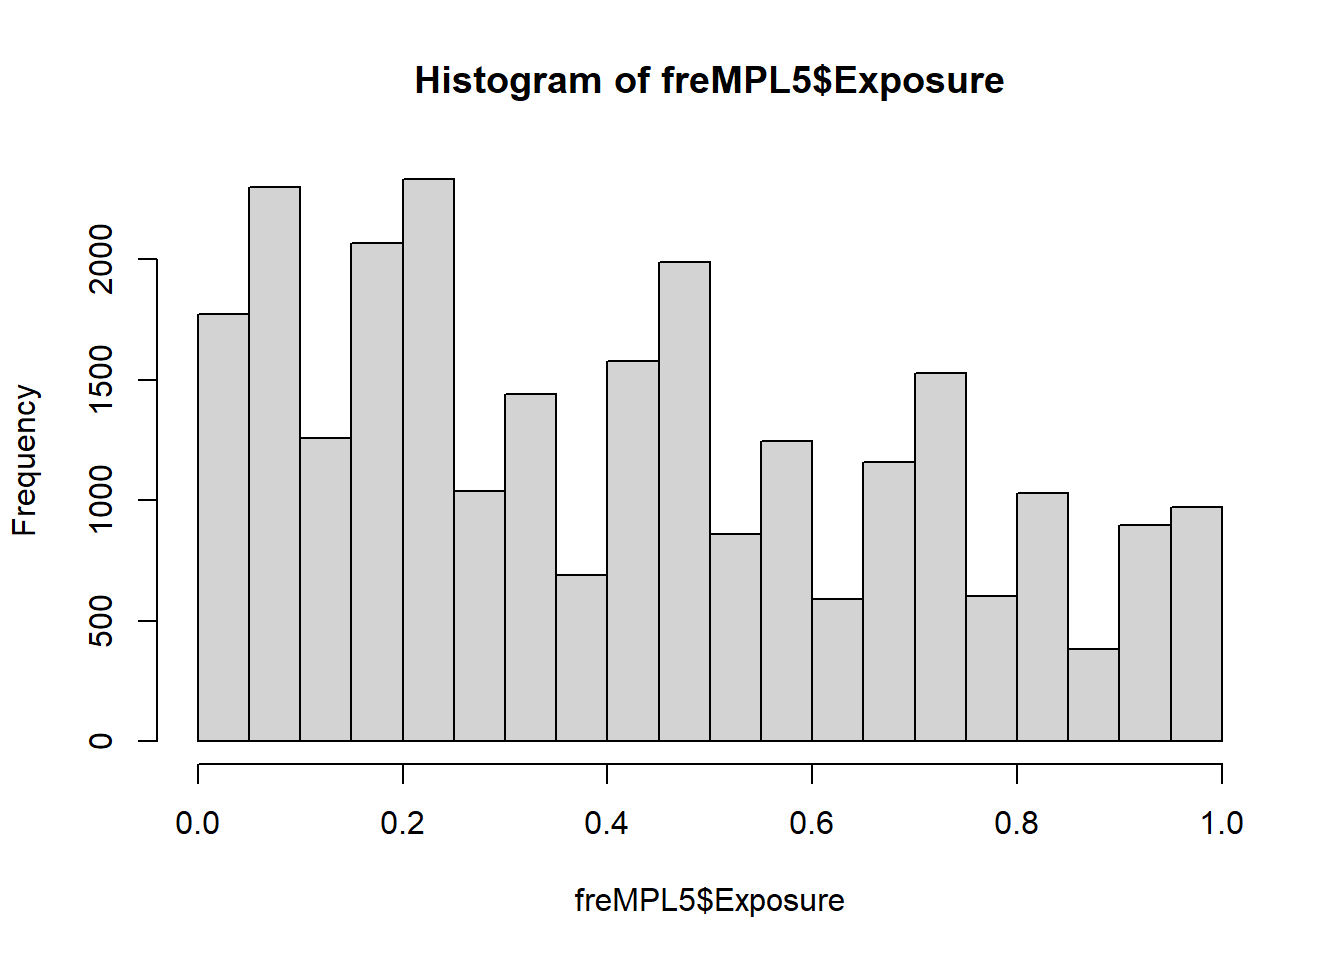
\includegraphics{GLM_sinistralité_Indicatrice_files/figure-latex/unnamed-chunk-27-1.pdf}

\hypertarget{table-de-confusion}{%
\subsubsection{Table de confusion}\label{table-de-confusion}}

\hypertarget{sur-le-jeu-de-donnuxe9es-train-1}{%
\paragraph{Sur le jeu de données
train}\label{sur-le-jeu-de-donnuxe9es-train-1}}

\begin{Shaded}
\begin{Highlighting}[]
\NormalTok{estimation }\OtherTok{\textless{}{-}}\NormalTok{ modFull}\SpecialCharTok{$}\NormalTok{fitted.values}
\FunctionTok{hist}\NormalTok{(estimation)}
\end{Highlighting}
\end{Shaded}

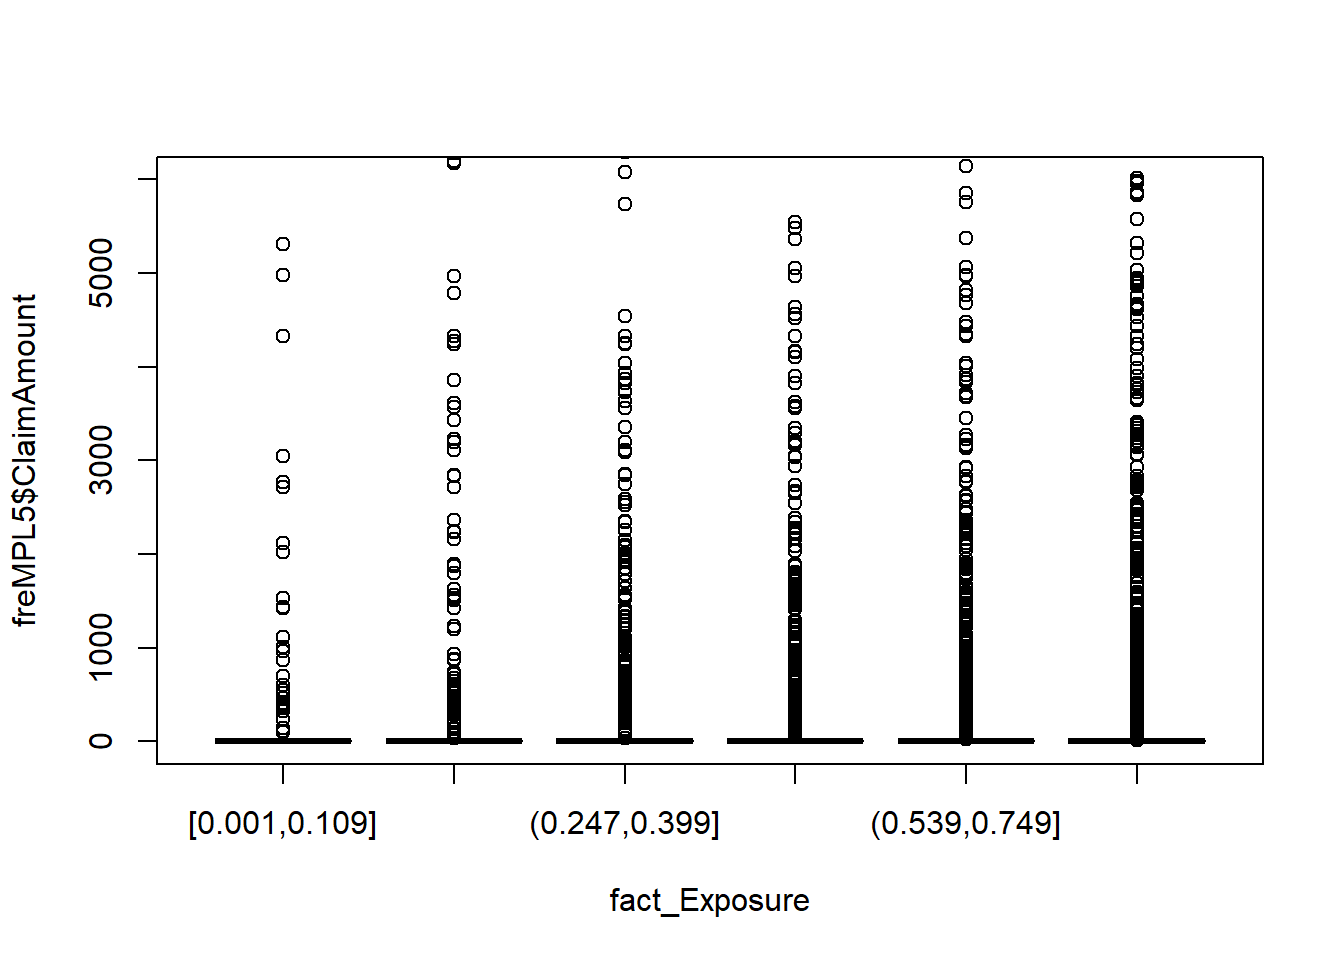
\includegraphics{GLM_sinistralité_Indicatrice_files/figure-latex/unnamed-chunk-28-1.pdf}

\begin{Shaded}
\begin{Highlighting}[]
\NormalTok{score }\OtherTok{\textless{}{-}} \FunctionTok{ifelse}\NormalTok{(}\FunctionTok{predict}\NormalTok{(modFull,train,}\AttributeTok{type=}\StringTok{"response"}\NormalTok{) }\SpecialCharTok{\textgreater{}}\NormalTok{.}\DecValTok{1}\NormalTok{, }\DecValTok{1}\NormalTok{, }\DecValTok{0}\NormalTok{)}
\NormalTok{confusion.mat }\OtherTok{=} \FunctionTok{table}\NormalTok{(train}\SpecialCharTok{$}\NormalTok{ClaimInd, score)  }
\NormalTok{fauxneg }\OtherTok{=}\NormalTok{ confusion.mat[}\DecValTok{2}\NormalTok{,}\DecValTok{1}\NormalTok{]}
\NormalTok{fauxpos }\OtherTok{=}\NormalTok{ confusion.mat[}\DecValTok{1}\NormalTok{,}\DecValTok{2}\NormalTok{]}
\NormalTok{vraisneg }\OtherTok{=}\NormalTok{ confusion.mat[}\DecValTok{1}\NormalTok{,}\DecValTok{1}\NormalTok{]}
\NormalTok{vraispos }\OtherTok{=}\NormalTok{ confusion.mat[}\DecValTok{2}\NormalTok{,}\DecValTok{2}\NormalTok{]}
\NormalTok{(}\AttributeTok{txerr =}\NormalTok{ (fauxneg}\SpecialCharTok{+}\NormalTok{fauxpos) }\SpecialCharTok{/}\NormalTok{ (fauxneg}\SpecialCharTok{+}\NormalTok{fauxpos}\SpecialCharTok{+}\NormalTok{vraisneg}\SpecialCharTok{+}\NormalTok{vraispos))}
\end{Highlighting}
\end{Shaded}

\begin{verbatim}
## [1] 0.3174711
\end{verbatim}

\begin{Shaded}
\begin{Highlighting}[]
\NormalTok{sensibilite }\OtherTok{\textless{}{-}}\NormalTok{ vraispos }\SpecialCharTok{/}\NormalTok{ (vraispos }\SpecialCharTok{+}\NormalTok{ fauxneg)   }
\NormalTok{precision }\OtherTok{\textless{}{-}}\NormalTok{ vraispos }\SpecialCharTok{/}\NormalTok{ (vraispos }\SpecialCharTok{+}\NormalTok{ fauxpos) }
\NormalTok{specificite }\OtherTok{\textless{}{-}}\NormalTok{ vraisneg }\SpecialCharTok{/}\NormalTok{ (vraisneg }\SpecialCharTok{+}\NormalTok{ fauxpos)}

\NormalTok{confusion.mat}
\end{Highlighting}
\end{Shaded}

\begin{verbatim}
##    score
##         0     1
##   0 13206  5483
##   1  1055   850
\end{verbatim}

\hypertarget{sur-le-jeu-de-donnuxe9es-test-1}{%
\paragraph{Sur le jeu de données
test}\label{sur-le-jeu-de-donnuxe9es-test-1}}

\begin{Shaded}
\begin{Highlighting}[]
\NormalTok{estimation }\OtherTok{\textless{}{-}}\NormalTok{ modFull}\SpecialCharTok{$}\NormalTok{fitted.values}
\FunctionTok{hist}\NormalTok{(estimation)}
\end{Highlighting}
\end{Shaded}

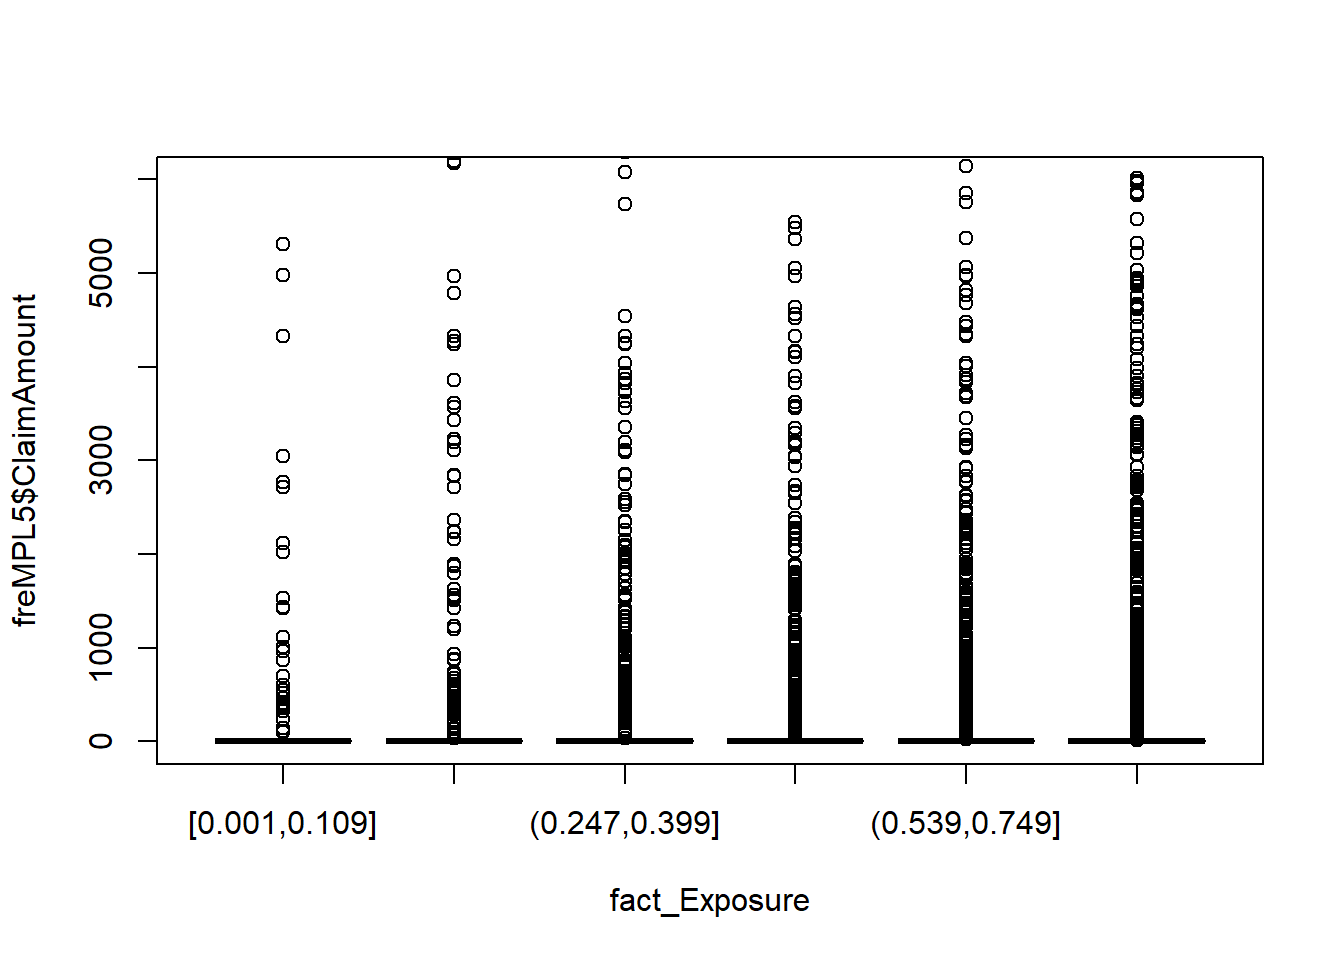
\includegraphics{GLM_sinistralité_Indicatrice_files/figure-latex/unnamed-chunk-29-1.pdf}

\begin{Shaded}
\begin{Highlighting}[]
\NormalTok{score }\OtherTok{\textless{}{-}} \FunctionTok{ifelse}\NormalTok{(}\FunctionTok{predict}\NormalTok{(modFull,test,}\AttributeTok{type=}\StringTok{"response"}\NormalTok{) }\SpecialCharTok{\textgreater{}}\NormalTok{.}\DecValTok{2}\NormalTok{, }\DecValTok{1}\NormalTok{, }\DecValTok{0}\NormalTok{)}
\NormalTok{confusion.mat }\OtherTok{=} \FunctionTok{table}\NormalTok{(test}\SpecialCharTok{$}\NormalTok{ClaimInd, score)  }
\NormalTok{fauxneg }\OtherTok{=}\NormalTok{ confusion.mat[}\DecValTok{2}\NormalTok{,}\DecValTok{1}\NormalTok{]}
\NormalTok{fauxpos }\OtherTok{=}\NormalTok{ confusion.mat[}\DecValTok{1}\NormalTok{,}\DecValTok{2}\NormalTok{]}
\NormalTok{vraisneg }\OtherTok{=}\NormalTok{ confusion.mat[}\DecValTok{1}\NormalTok{,}\DecValTok{1}\NormalTok{]}
\NormalTok{vraispos }\OtherTok{=}\NormalTok{ confusion.mat[}\DecValTok{2}\NormalTok{,}\DecValTok{2}\NormalTok{]}
\NormalTok{(}\AttributeTok{txerr =}\NormalTok{ (fauxneg}\SpecialCharTok{+}\NormalTok{fauxpos) }\SpecialCharTok{/}\NormalTok{ (fauxneg}\SpecialCharTok{+}\NormalTok{fauxpos}\SpecialCharTok{+}\NormalTok{vraisneg}\SpecialCharTok{+}\NormalTok{vraispos))}
\end{Highlighting}
\end{Shaded}

\begin{verbatim}
## [1] 0.1045242
\end{verbatim}

\begin{Shaded}
\begin{Highlighting}[]
\NormalTok{sensibilite }\OtherTok{\textless{}{-}}\NormalTok{ vraispos }\SpecialCharTok{/}\NormalTok{ (vraispos }\SpecialCharTok{+}\NormalTok{ fauxneg)   }
\NormalTok{precision }\OtherTok{\textless{}{-}}\NormalTok{ vraispos }\SpecialCharTok{/}\NormalTok{ (vraispos }\SpecialCharTok{+}\NormalTok{ fauxpos) }
\NormalTok{specificite }\OtherTok{\textless{}{-}}\NormalTok{ vraisneg }\SpecialCharTok{/}\NormalTok{ (vraisneg }\SpecialCharTok{+}\NormalTok{ fauxpos)}

\NormalTok{confusion.mat}
\end{Highlighting}
\end{Shaded}

\begin{verbatim}
##    score
##        0    1
##   0 4589   26
##   1  510    3
\end{verbatim}

\hypertarget{cross-validation}{%
\subsection{Cross Validation}\label{cross-validation}}

\begin{Shaded}
\begin{Highlighting}[]
\NormalTok{fit.control }\OtherTok{\textless{}{-}} \FunctionTok{trainControl}\NormalTok{(}\AttributeTok{method =} \StringTok{"repeatedcv"}\NormalTok{, }\AttributeTok{number =} \DecValTok{5}\NormalTok{, }\AttributeTok{repeats =} \DecValTok{10}\NormalTok{)}

\NormalTok{fit }\OtherTok{\textless{}{-}} \FunctionTok{train}\NormalTok{(ClaimInd }\SpecialCharTok{\textasciitilde{}}\NormalTok{ MariStat}\SpecialCharTok{+}\NormalTok{Categ}\SpecialCharTok{+}\NormalTok{VehUsage}\SpecialCharTok{+}\NormalTok{HasKmLimit}\SpecialCharTok{+}\NormalTok{ClaimNbResp}\SpecialCharTok{+}\NormalTok{ClaimNbNonResp}\SpecialCharTok{+}\NormalTok{ClaimNbParking}\SpecialCharTok{+}\NormalTok{ClaimNbFireTheft}\SpecialCharTok{+}\NormalTok{ClaimNbWindscreen}\SpecialCharTok{+}\NormalTok{OutUseNb}\SpecialCharTok{+}\NormalTok{Risque}\SpecialCharTok{+}\NormalTok{BonusMalus}\SpecialCharTok{+}\NormalTok{DrivAge\_fact,}
    \AttributeTok{data =}\NormalTok{ train, }\AttributeTok{method =} \StringTok{"glm"}\NormalTok{, }
    \AttributeTok{family =} \StringTok{"binomial"}\NormalTok{, }\AttributeTok{trControl =}\NormalTok{ fit.control)}
\end{Highlighting}
\end{Shaded}

\begin{verbatim}
## Warning in train.default(x, y, weights = w, ...): You are trying to do
## regression and your outcome only has two possible values Are you trying to do
## classification? If so, use a 2 level factor as your outcome column.
\end{verbatim}

\begin{Shaded}
\begin{Highlighting}[]
\FunctionTok{summary}\NormalTok{(fit)}
\end{Highlighting}
\end{Shaded}

\begin{verbatim}
## 
## Call:
## NULL
## 
## Deviance Residuals: 
##     Min       1Q   Median       3Q      Max  
## -1.0117  -0.4634  -0.4102  -0.3735   2.5183  
## 
## Coefficients:
##                                   Estimate Std. Error z value Pr(>|z|)    
## (Intercept)                      -3.080639   0.295271 -10.433  < 2e-16 ***
## MariStatOther                     0.038152   0.077764   0.491 0.623699    
## Categ1                            0.572832   0.144055   3.976 6.99e-05 ***
## Categ2                            0.477981   0.165771   2.883 0.003934 ** 
## Categ3                            0.433797   0.132610   3.271 0.001071 ** 
## Categ4                            0.413109   0.169665   2.435 0.014898 *  
## `VehUsagePrivate+trip to office`  0.076346   0.086392   0.884 0.376851    
## VehUsageProfessional              0.335517   0.102044   3.288 0.001009 ** 
## `VehUsageProfessional run`        0.340185   0.148725   2.287 0.022176 *  
## HasKmLimit1                      -0.125699   0.105371  -1.193 0.232900    
## ClaimNbResp                       0.125942   0.046818   2.690 0.007145 ** 
## ClaimNbNonResp                    0.136365   0.036174   3.770 0.000163 ***
## ClaimNbParking                    0.246198   0.070007   3.517 0.000437 ***
## ClaimNbFireTheft                  0.216801   0.074214   2.921 0.003486 ** 
## ClaimNbWindscreen                 0.102365   0.033136   3.089 0.002007 ** 
## OutUseNb                          0.049930   0.034046   1.467 0.142499    
## Risque1                          -0.147936   0.135539  -1.091 0.275068    
## Risque2                           0.009096   0.143161   0.064 0.949340    
## Risque3                           0.024434   0.148431   0.165 0.869246    
## Risque4                           0.283316   0.172630   1.641 0.100761    
## BonusMalus                        0.005907   0.002131   2.772 0.005577 ** 
## `DrivAge_fact(25,30]`            -0.084739   0.155177  -0.546 0.585011    
## `DrivAge_fact(30,35]`            -0.389282   0.158830  -2.451 0.014249 *  
## `DrivAge_fact(35,40]`            -0.309196   0.162676  -1.901 0.057344 .  
## `DrivAge_fact(40,45]`            -0.088170   0.163972  -0.538 0.590776    
## `DrivAge_fact(45,50]`            -0.174425   0.165911  -1.051 0.293115    
## `DrivAge_fact(50,58]`            -0.297892   0.160850  -1.852 0.064027 .  
## `DrivAge_fact(58,65]`            -0.145346   0.172500  -0.843 0.399459    
## `DrivAge_fact(65,120]`           -0.271711   0.188506  -1.441 0.149473    
## ---
## Signif. codes:  0 '***' 0.001 '**' 0.01 '*' 0.05 '.' 0.1 ' ' 1
## 
## (Dispersion parameter for binomial family taken to be 1)
## 
##     Null deviance: 12698  on 20593  degrees of freedom
## Residual deviance: 12487  on 20565  degrees of freedom
## AIC: 12545
## 
## Number of Fisher Scoring iterations: 5
\end{verbatim}

\hypertarget{moduxe9lisation-de-sinistres2-variable-dans-mathbbn}{%
\section{\texorpdfstring{2) Modélisation de \texttt{Sinistres2}
(variable dans
\(\mathbb{N}\))}{2) Modélisation de Sinistres2 (variable dans \textbackslash mathbb\{N\})}}\label{moduxe9lisation-de-sinistres2-variable-dans-mathbbn}}

\hypertarget{a-moduxe9lisation-avec-une-poisson}{%
\subsection{a) Modélisation avec une
Poisson}\label{a-moduxe9lisation-avec-une-poisson}}

\begin{Shaded}
\begin{Highlighting}[]
\FunctionTok{summary}\NormalTok{(freMPL5}\SpecialCharTok{$}\NormalTok{Sinistres)}
\end{Highlighting}
\end{Shaded}

\begin{verbatim}
##     Min.  1st Qu.   Median     Mean  3rd Qu.     Max. 
##   0.0000   0.0000   0.0000   0.2707   0.0000 500.0000
\end{verbatim}

\begin{Shaded}
\begin{Highlighting}[]
\NormalTok{bornes }\OtherTok{=} \FunctionTok{seq}\NormalTok{(}\DecValTok{0}\NormalTok{,}\DecValTok{501}\NormalTok{,}\DecValTok{1}\NormalTok{)}
\FunctionTok{hist}\NormalTok{(freMPL5}\SpecialCharTok{$}\NormalTok{Sinistres)}
\end{Highlighting}
\end{Shaded}

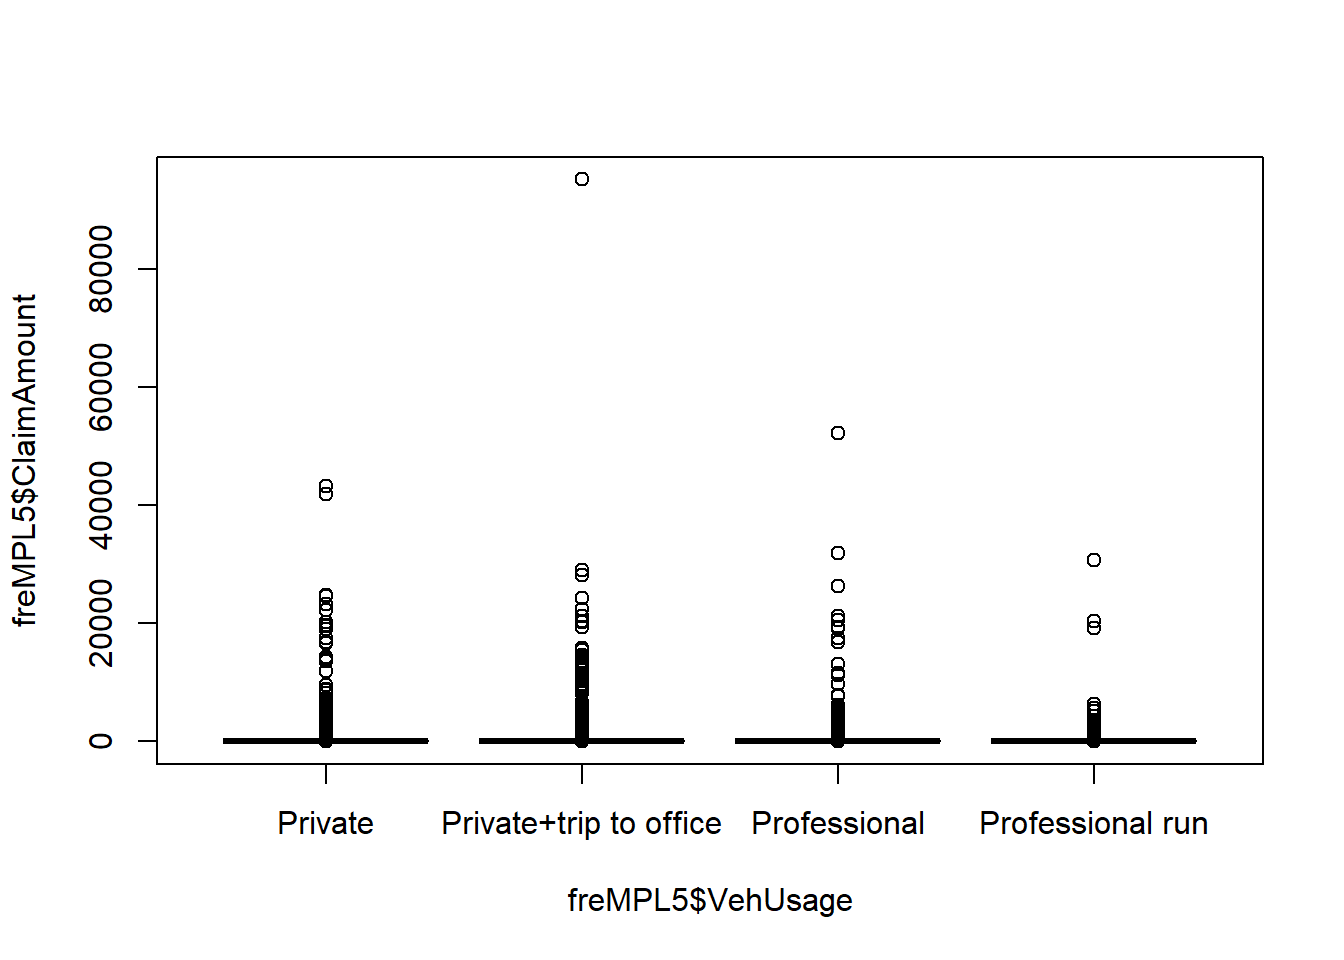
\includegraphics{GLM_sinistralité_Indicatrice_files/figure-latex/unnamed-chunk-31-1.pdf}

\begin{Shaded}
\begin{Highlighting}[]
\FunctionTok{hist}\NormalTok{(freMPL5}\SpecialCharTok{$}\NormalTok{Sinistres, }\AttributeTok{breaks=}\NormalTok{bornes, }\AttributeTok{xlim=}\FunctionTok{c}\NormalTok{(}\DecValTok{0}\NormalTok{,}\DecValTok{10}\NormalTok{))}
\end{Highlighting}
\end{Shaded}

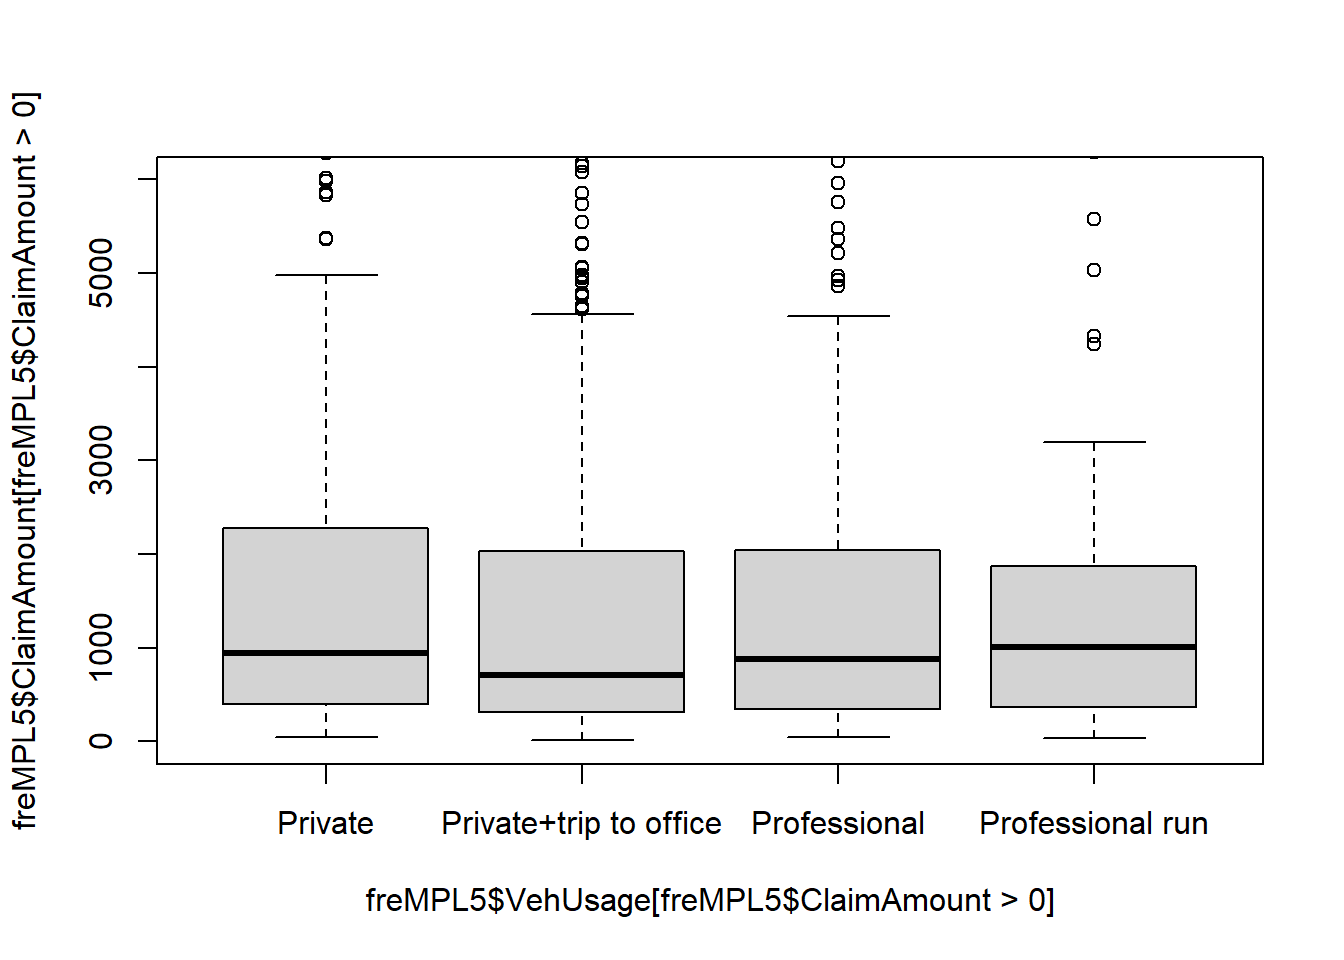
\includegraphics{GLM_sinistralité_Indicatrice_files/figure-latex/unnamed-chunk-31-2.pdf}

\begin{Shaded}
\begin{Highlighting}[]
\FunctionTok{hist}\NormalTok{(freMPL5}\SpecialCharTok{$}\NormalTok{Sinistres, }\AttributeTok{breaks=}\NormalTok{bornes, }\AttributeTok{xlim=}\FunctionTok{c}\NormalTok{(}\DecValTok{0}\NormalTok{,}\DecValTok{10}\NormalTok{), }\AttributeTok{ylim =} \FunctionTok{c}\NormalTok{(}\DecValTok{0}\NormalTok{,}\DecValTok{2000}\NormalTok{))}
\end{Highlighting}
\end{Shaded}

\includegraphics{GLM_sinistralité_Indicatrice_files/figure-latex/unnamed-chunk-31-3.pdf}

\hypertarget{lien-log-lien-canonique}{%
\subsubsection{Lien log (lien
canonique)}\label{lien-log-lien-canonique}}

\begin{Shaded}
\begin{Highlighting}[]
\NormalTok{mod0\_2 }\OtherTok{\textless{}{-}} \FunctionTok{glm}\NormalTok{(Sinistres2 }\SpecialCharTok{\textasciitilde{}} \DecValTok{1}\NormalTok{, }\AttributeTok{data =}\NormalTok{ train, }\AttributeTok{family =} \FunctionTok{poisson}\NormalTok{(}\AttributeTok{link =} \StringTok{"log"}\NormalTok{))}
\FunctionTok{summary}\NormalTok{(mod0\_2)}
\end{Highlighting}
\end{Shaded}

\begin{verbatim}
## 
## Call:
## glm(formula = Sinistres2 ~ 1, family = poisson(link = "log"), 
##     data = train)
## 
## Deviance Residuals: 
##    Min      1Q  Median      3Q     Max  
## -0.737  -0.737  -0.737  -0.737  80.740  
## 
## Coefficients:
##             Estimate Std. Error z value Pr(>|z|)    
## (Intercept) -1.30384    0.01337  -97.49   <2e-16 ***
## ---
## Signif. codes:  0 '***' 0.001 '**' 0.01 '*' 0.05 '.' 0.1 ' ' 1
## 
## (Dispersion parameter for poisson family taken to be 1)
## 
##     Null deviance: 38640  on 20593  degrees of freedom
## Residual deviance: 38640  on 20593  degrees of freedom
## AIC: 43484
## 
## Number of Fisher Scoring iterations: 7
\end{verbatim}

\begin{Shaded}
\begin{Highlighting}[]
\SpecialCharTok{{-}}\DecValTok{2}\SpecialCharTok{*}\FunctionTok{as.numeric}\NormalTok{(}\FunctionTok{logLik}\NormalTok{(mod0\_2))}
\end{Highlighting}
\end{Shaded}

\begin{verbatim}
## [1] 43481.87
\end{verbatim}

\begin{Shaded}
\begin{Highlighting}[]
\NormalTok{modFull\_2 }\OtherTok{\textless{}{-}} \FunctionTok{glm}\NormalTok{(Sinistres2 }\SpecialCharTok{\textasciitilde{}}\NormalTok{ MariStat}\SpecialCharTok{+}\NormalTok{VehUsage}\SpecialCharTok{+}\NormalTok{HasKmLimit}\SpecialCharTok{+}\NormalTok{ClaimNbResp}\SpecialCharTok{+}\NormalTok{ClaimNbNonResp}\SpecialCharTok{+}\NormalTok{ClaimNbParking}\SpecialCharTok{+}\NormalTok{ClaimNbFireTheft}\SpecialCharTok{+}\NormalTok{ClaimNbWindscreen}\SpecialCharTok{+}\NormalTok{OutUseNb}\SpecialCharTok{+}\NormalTok{BonusMalus}\SpecialCharTok{+}\NormalTok{Risque}\SpecialCharTok{+}\NormalTok{DrivAge\_fact}\SpecialCharTok{+}\NormalTok{Categ, }\AttributeTok{data =}\NormalTok{ train, }\AttributeTok{family =} \FunctionTok{poisson}\NormalTok{(}\AttributeTok{link =} \StringTok{"log"}\NormalTok{))}
\FunctionTok{summary}\NormalTok{(modFull\_2)}
\end{Highlighting}
\end{Shaded}

\begin{verbatim}
## 
## Call:
## glm(formula = Sinistres2 ~ MariStat + VehUsage + HasKmLimit + 
##     ClaimNbResp + ClaimNbNonResp + ClaimNbParking + ClaimNbFireTheft + 
##     ClaimNbWindscreen + OutUseNb + BonusMalus + Risque + DrivAge_fact + 
##     Categ, family = poisson(link = "log"), data = train)
## 
## Deviance Residuals: 
##    Min      1Q  Median      3Q     Max  
## -5.174  -0.720  -0.545  -0.483  58.054  
## 
## Coefficients:
##                                  Estimate Std. Error z value Pr(>|z|)    
## (Intercept)                    -1.5608264  0.1706646  -9.146  < 2e-16 ***
## MariStatOther                   0.0729785  0.0463852   1.573 0.115646    
## VehUsagePrivate+trip to office -0.1224106  0.0494015  -2.478 0.013217 *  
## VehUsageProfessional            0.2756465  0.0548864   5.022 5.11e-07 ***
## VehUsageProfessional run       -0.7125922  0.0870696  -8.184 2.74e-16 ***
## HasKmLimit1                    -0.1711479  0.0685600  -2.496 0.012549 *  
## ClaimNbResp                    -0.1036668  0.0281241  -3.686 0.000228 ***
## ClaimNbNonResp                  0.5709308  0.0139603  40.897  < 2e-16 ***
## ClaimNbParking                  0.1124558  0.0422659   2.661 0.007798 ** 
## ClaimNbFireTheft               -0.2330213  0.0494395  -4.713 2.44e-06 ***
## ClaimNbWindscreen               0.1145049  0.0173010   6.618 3.63e-11 ***
## OutUseNb                        0.0347003  0.0177326   1.957 0.050363 .  
## BonusMalus                      0.0008187  0.0012777   0.641 0.521673    
## Risque1                        -0.0707266  0.0769473  -0.919 0.358014    
## Risque2                        -0.1605381  0.0815934  -1.968 0.049121 *  
## Risque3                        -0.5929143  0.0880779  -6.732 1.68e-11 ***
## Risque4                        -0.3024983  0.1061617  -2.849 0.004380 ** 
## DrivAge_fact(25,30]            -0.2254204  0.0833209  -2.705 0.006821 ** 
## DrivAge_fact(30,35]            -0.8814792  0.0899556  -9.799  < 2e-16 ***
## DrivAge_fact(35,40]            -0.9265070  0.0926617  -9.999  < 2e-16 ***
## DrivAge_fact(40,45]            -0.7032381  0.0915991  -7.677 1.62e-14 ***
## DrivAge_fact(45,50]             0.2574291  0.0866032   2.973 0.002954 ** 
## DrivAge_fact(50,58]            -0.9558954  0.0900264 -10.618  < 2e-16 ***
## DrivAge_fact(58,65]            -0.8542331  0.0975878  -8.753  < 2e-16 ***
## DrivAge_fact(65,120]           -0.8947887  0.1067553  -8.382  < 2e-16 ***
## Categ1                          1.5853872  0.0821607  19.296  < 2e-16 ***
## Categ2                          0.1155137  0.1044809   1.106 0.268901    
## Categ3                          0.4503152  0.0807345   5.578 2.44e-08 ***
## Categ4                          0.4670674  0.1035072   4.512 6.41e-06 ***
## ---
## Signif. codes:  0 '***' 0.001 '**' 0.01 '*' 0.05 '.' 0.1 ' ' 1
## 
## (Dispersion parameter for poisson family taken to be 1)
## 
##     Null deviance: 38640  on 20593  degrees of freedom
## Residual deviance: 33821  on 20565  degrees of freedom
## AIC: 38721
## 
## Number of Fisher Scoring iterations: 9
\end{verbatim}

\begin{Shaded}
\begin{Highlighting}[]
\SpecialCharTok{{-}}\DecValTok{2}\SpecialCharTok{*}\FunctionTok{as.numeric}\NormalTok{(}\FunctionTok{logLik}\NormalTok{(modFull\_2))}
\end{Highlighting}
\end{Shaded}

\begin{verbatim}
## [1] 38663.13
\end{verbatim}

Avec les intéractions entre DrivAge\_fact et Categ, cela permet
d'obtenir un meilleur critère d'AIC tout en conservant un temps de
calcul cohérent.

\begin{Shaded}
\begin{Highlighting}[]
\NormalTok{modBoth\_2 }\OtherTok{=} \FunctionTok{step}\NormalTok{(modFull\_2, mod0\_2, }\AttributeTok{trace=}\NormalTok{F, }\AttributeTok{direction =} \FunctionTok{c}\NormalTok{(}\StringTok{\textquotesingle{}both\textquotesingle{}}\NormalTok{))}
\FunctionTok{summary}\NormalTok{(modBoth\_2)}
\end{Highlighting}
\end{Shaded}

\begin{verbatim}
## 
## Call:
## glm(formula = Sinistres2 ~ MariStat + VehUsage + HasKmLimit + 
##     ClaimNbResp + ClaimNbNonResp + ClaimNbParking + ClaimNbFireTheft + 
##     ClaimNbWindscreen + OutUseNb + Risque + DrivAge_fact + Categ, 
##     family = poisson(link = "log"), data = train)
## 
## Deviance Residuals: 
##    Min      1Q  Median      3Q     Max  
## -5.208  -0.720  -0.545  -0.483  58.045  
## 
## Coefficients:
##                                Estimate Std. Error z value Pr(>|z|)    
## (Intercept)                    -1.49122    0.13162 -11.330  < 2e-16 ***
## MariStatOther                   0.07070    0.04625   1.529  0.12635    
## VehUsagePrivate+trip to office -0.12263    0.04941  -2.482  0.01306 *  
## VehUsageProfessional            0.27521    0.05488   5.015 5.30e-07 ***
## VehUsageProfessional run       -0.71566    0.08693  -8.232  < 2e-16 ***
## HasKmLimit1                    -0.17137    0.06856  -2.500  0.01243 *  
## ClaimNbResp                    -0.09579    0.02527  -3.790  0.00015 ***
## ClaimNbNonResp                  0.57086    0.01395  40.915  < 2e-16 ***
## ClaimNbParking                  0.11195    0.04226   2.649  0.00808 ** 
## ClaimNbFireTheft               -0.23301    0.04944  -4.713 2.44e-06 ***
## ClaimNbWindscreen               0.11428    0.01730   6.604 4.00e-11 ***
## OutUseNb                        0.03511    0.01772   1.981  0.04758 *  
## Risque1                        -0.07077    0.07695  -0.920  0.35774    
## Risque2                        -0.15988    0.08159  -1.960  0.05004 .  
## Risque3                        -0.59061    0.08800  -6.711 1.93e-11 ***
## Risque4                        -0.30418    0.10613  -2.866  0.00415 ** 
## DrivAge_fact(25,30]            -0.23152    0.08278  -2.797  0.00516 ** 
## DrivAge_fact(30,35]            -0.89698    0.08666 -10.350  < 2e-16 ***
## DrivAge_fact(35,40]            -0.94707    0.08695 -10.892  < 2e-16 ***
## DrivAge_fact(40,45]            -0.72714    0.08366  -8.691  < 2e-16 ***
## DrivAge_fact(45,50]             0.23175    0.07677   3.019  0.00254 ** 
## DrivAge_fact(50,58]            -0.98239    0.07996 -12.286  < 2e-16 ***
## DrivAge_fact(58,65]            -0.88003    0.08890  -9.900  < 2e-16 ***
## DrivAge_fact(65,120]           -0.92046    0.09897  -9.301  < 2e-16 ***
## Categ1                          1.58654    0.08214  19.316  < 2e-16 ***
## Categ2                          0.11630    0.10447   1.113  0.26562    
## Categ3                          0.45067    0.08073   5.582 2.37e-08 ***
## Categ4                          0.46576    0.10348   4.501 6.76e-06 ***
## ---
## Signif. codes:  0 '***' 0.001 '**' 0.01 '*' 0.05 '.' 0.1 ' ' 1
## 
## (Dispersion parameter for poisson family taken to be 1)
## 
##     Null deviance: 38640  on 20593  degrees of freedom
## Residual deviance: 33822  on 20566  degrees of freedom
## AIC: 38720
## 
## Number of Fisher Scoring iterations: 9
\end{verbatim}

\begin{Shaded}
\begin{Highlighting}[]
\SpecialCharTok{{-}}\DecValTok{2}\SpecialCharTok{*}\FunctionTok{as.numeric}\NormalTok{(}\FunctionTok{logLik}\NormalTok{(modBoth\_2))}
\end{Highlighting}
\end{Shaded}

\begin{verbatim}
## [1] 38663.54
\end{verbatim}

Remarque : Certaines interactions ont un coefficient indefini car aucun
individu ne possède ces caractères dans l'échantilllon \texttt{train}.

D'autres une p-value très faible mais un coefficient élevé (en valeur
absolue). Cela veut dire qu'il y a pas trop peu d'individus dans
l'échantillon \texttt{train}. Nous devrons faire attention à cela
puisque ça risque de mener à un surapprentissage. Nous ne conserverons
donc que les interactions qui sont suffisamment représentatives dans
l'échantillon \texttt{freMPL5}.

Cependant, continuons avant cela d'explorer les modèles. Ensuite nous en
sélectionnerons un et nous l'améliorerons.

\begin{Shaded}
\begin{Highlighting}[]
\FunctionTok{plot}\NormalTok{(modBoth\_2)}
\end{Highlighting}
\end{Shaded}

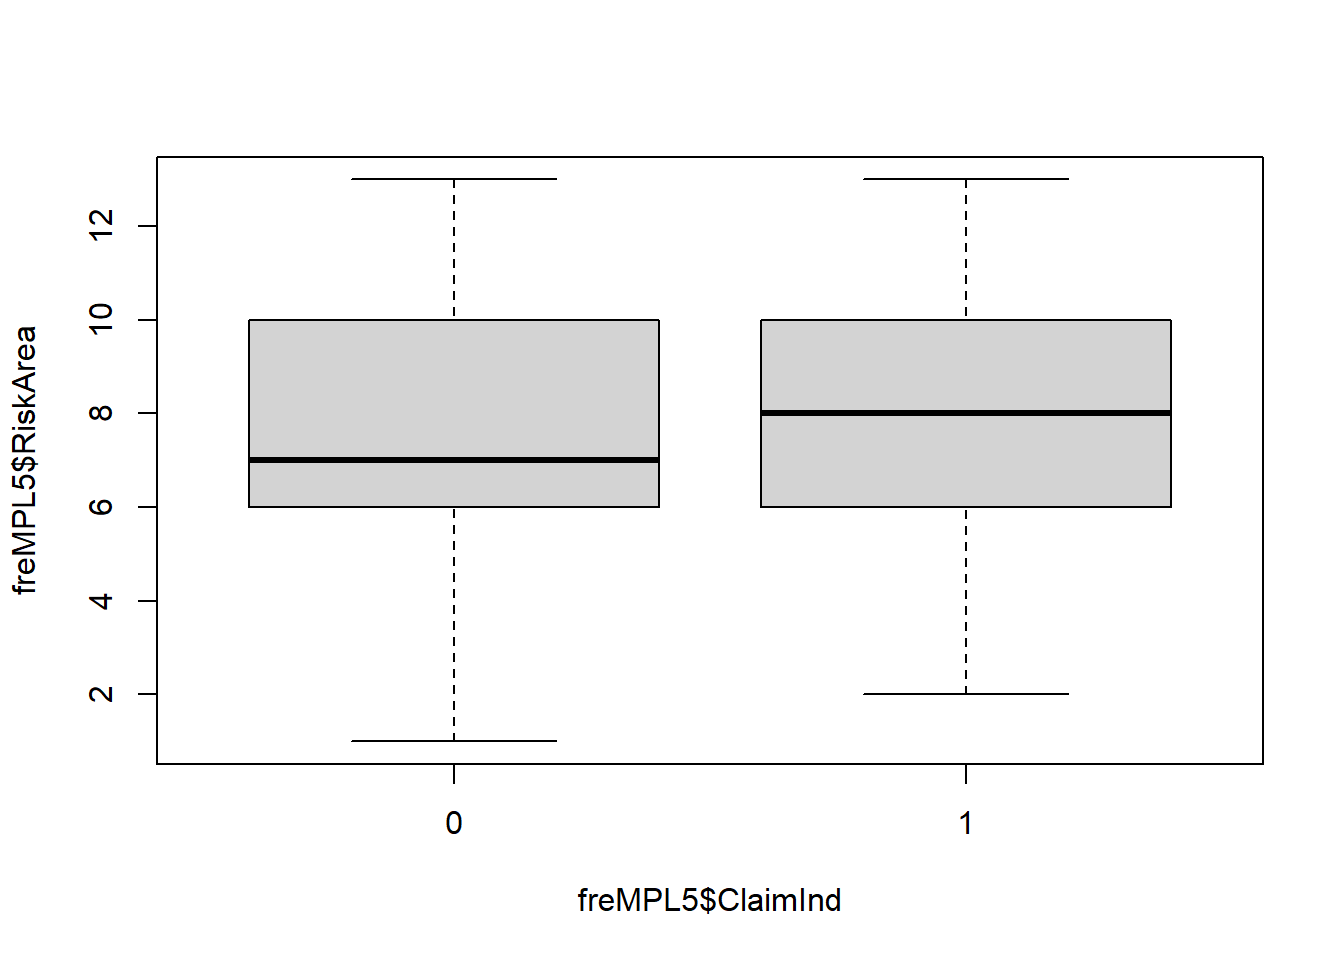
\includegraphics{GLM_sinistralité_Indicatrice_files/figure-latex/unnamed-chunk-38-1.pdf}
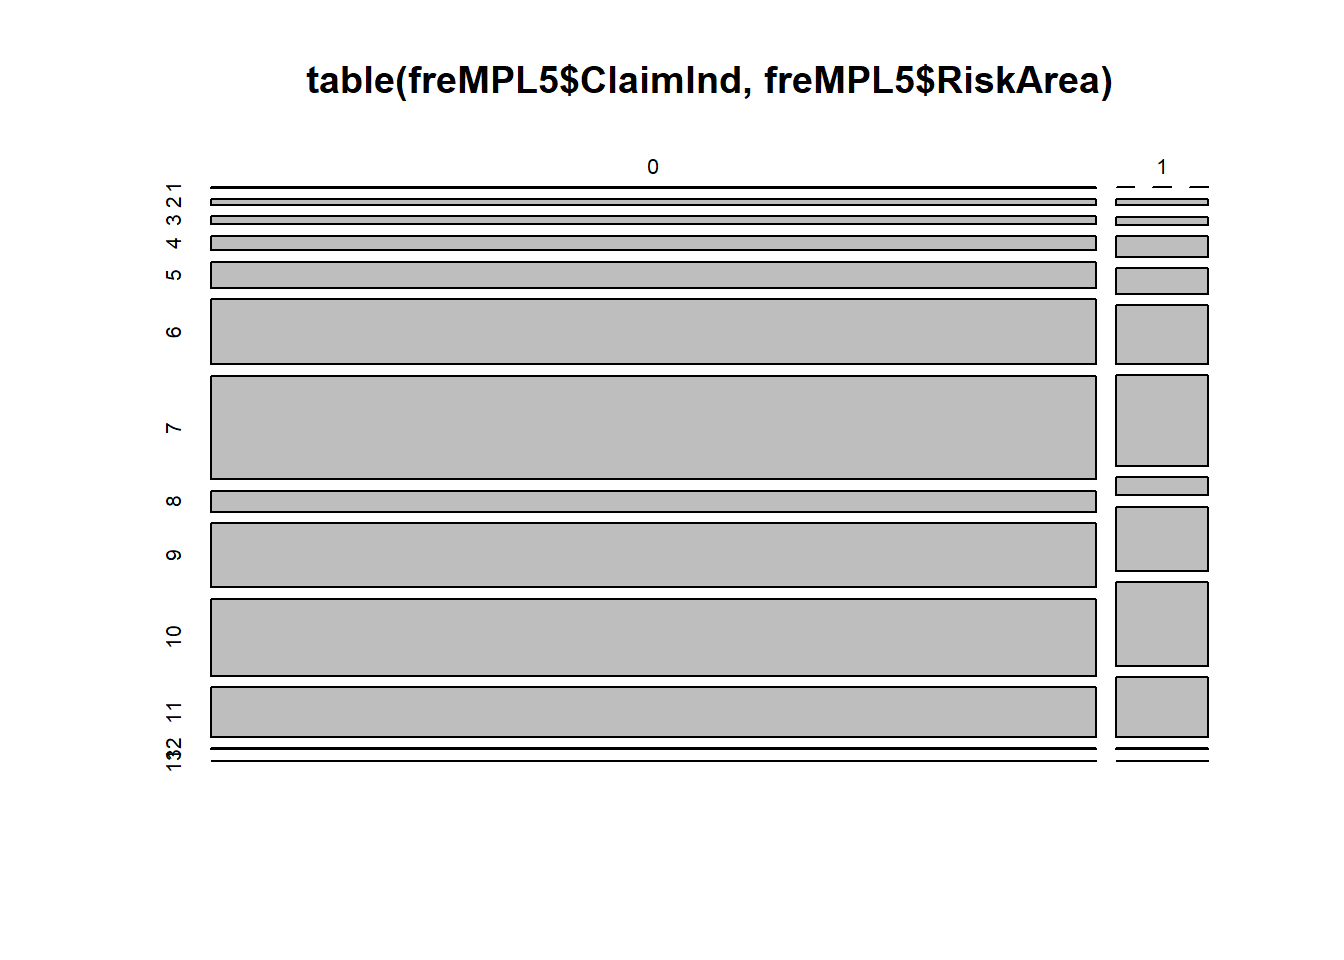
\includegraphics{GLM_sinistralité_Indicatrice_files/figure-latex/unnamed-chunk-38-2.pdf}
\includegraphics{GLM_sinistralité_Indicatrice_files/figure-latex/unnamed-chunk-38-3.pdf}
\includegraphics{GLM_sinistralité_Indicatrice_files/figure-latex/unnamed-chunk-38-4.pdf}

\begin{Shaded}
\begin{Highlighting}[]
\NormalTok{lmb }\OtherTok{=} \FunctionTok{mean}\NormalTok{(freMPL5}\SpecialCharTok{$}\NormalTok{Sinistres2)}
\FunctionTok{qqplot}\NormalTok{ (freMPL5}\SpecialCharTok{$}\NormalTok{Sinistres2, }\FunctionTok{qpois}\NormalTok{(}\FunctionTok{ppoints}\NormalTok{(freMPL5}\SpecialCharTok{$}\NormalTok{Sinistres2), }\AttributeTok{lambda =}\NormalTok{ lmb),}
            \AttributeTok{xlab =}\StringTok{"Sinistralité observées"}\NormalTok{,}
        \AttributeTok{main =}\StringTok{"Graphique des quantiles pour la sinistralité."}\NormalTok{, }\AttributeTok{xlim =} \FunctionTok{c}\NormalTok{(}\DecValTok{0}\NormalTok{,}\DecValTok{50}\NormalTok{))}
\FunctionTok{abline}\NormalTok{ (}\AttributeTok{a=}\DecValTok{0}\NormalTok{,}\AttributeTok{b=}\DecValTok{1}\NormalTok{, }\AttributeTok{col =}\StringTok{"red"}\NormalTok{)}
\end{Highlighting}
\end{Shaded}

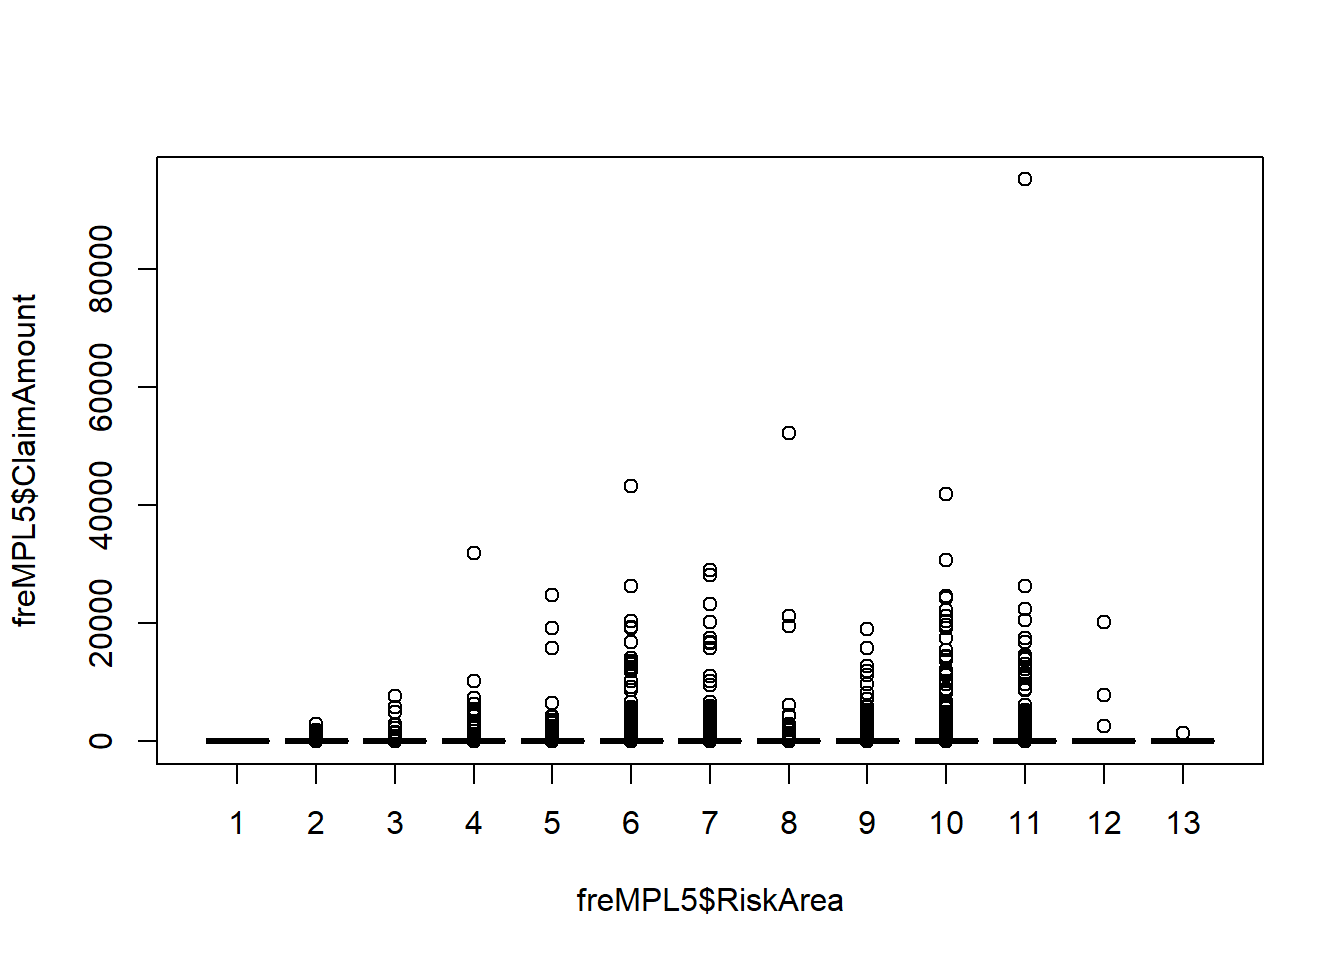
\includegraphics{GLM_sinistralité_Indicatrice_files/figure-latex/unnamed-chunk-39-1.pdf}

Remarque : Nous avons tronquer xlim afin d'avoir une interprétation
possible et visuelle. Sinon, il y avait quelques éléments qui allait
bien trop loin (valeurs trop extrèmes).

Avec ce graphique des qqplot. On remarque bien que la loi de Poisson
n'est pas adaptée à cette modélisation. En effet, il y a quelques
observations qui sont très élevés, qui faussent la moyenne (appelée lmb
ici qui est aussi le paramètre de la loi). Alors nous allons tenter de
modéliser en enlevant dans un premier temps les données qui dépassent un
certain seuil.

\begin{Shaded}
\begin{Highlighting}[]
\NormalTok{RMSE\_2\_train }\OtherTok{\textless{}{-}} \FunctionTok{sqrt}\NormalTok{(}\FunctionTok{mean}\NormalTok{(modBoth\_2}\SpecialCharTok{$}\NormalTok{residuals}\SpecialCharTok{\^{}}\DecValTok{2}\NormalTok{))}
\NormalTok{RMSE\_2\_train}
\end{Highlighting}
\end{Shaded}

\begin{verbatim}
## [1] 6.445786
\end{verbatim}

\hypertarget{lien-identituxe9}{%
\subsubsection{Lien identité}\label{lien-identituxe9}}

\begin{Shaded}
\begin{Highlighting}[]
\NormalTok{mod0\_identité }\OtherTok{\textless{}{-}} \FunctionTok{glm}\NormalTok{(Sinistres2 }\SpecialCharTok{\textasciitilde{}} \DecValTok{1}\NormalTok{, }\AttributeTok{data =}\NormalTok{ train, }\AttributeTok{family =} \FunctionTok{poisson}\NormalTok{(}\AttributeTok{link =} \StringTok{"identity"}\NormalTok{))}
\FunctionTok{summary}\NormalTok{(mod0\_identité)}
\end{Highlighting}
\end{Shaded}

\begin{verbatim}
## 
## Call:
## glm(formula = Sinistres2 ~ 1, family = poisson(link = "identity"), 
##     data = train)
## 
## Deviance Residuals: 
##    Min      1Q  Median      3Q     Max  
## -0.737  -0.737  -0.737  -0.737  80.740  
## 
## Coefficients:
##             Estimate Std. Error z value Pr(>|z|)    
## (Intercept) 0.271487   0.003631   74.77   <2e-16 ***
## ---
## Signif. codes:  0 '***' 0.001 '**' 0.01 '*' 0.05 '.' 0.1 ' ' 1
## 
## (Dispersion parameter for poisson family taken to be 1)
## 
##     Null deviance: 38640  on 20593  degrees of freedom
## Residual deviance: 38640  on 20593  degrees of freedom
## AIC: 43484
## 
## Number of Fisher Scoring iterations: 3
\end{verbatim}

\begin{Shaded}
\begin{Highlighting}[]
\CommentTok{\#modFull\_identité \textless{}{-} glm(Sinistres2 \textasciitilde{} MariStat+Categ+VehUsage+HasKmLimit+ClaimNbResp+ClaimNbNonResp+ClaimNbParking+ClaimNbFireTheft+ClaimNbWindscreen+OutUseNb+RiskArea+BonusMalus+DrivAge\_fact, data = train, family = poisson(link = "identity"))}
\CommentTok{\#summary(modFull\_identité)}
\end{Highlighting}
\end{Shaded}

Il y a une erreur. Est-ce par rapport au fait qu'il ne pervient pas à
trouver des valeurs pour les coefficients et donc que la méthode n'est
pas convergente ?

\hypertarget{lien-sqrt}{%
\subsubsection{Lien sqrt}\label{lien-sqrt}}

Remarque : d'après la documentation R, on ne pourra pas utiliser
d'autres liens car ``the \texttt{poisson} family accepts the links
\texttt{log}, \texttt{identity}, and \texttt{sqrt}''.

\begin{Shaded}
\begin{Highlighting}[]
\NormalTok{mod0\_sqrt }\OtherTok{\textless{}{-}} \FunctionTok{glm}\NormalTok{(Sinistres2 }\SpecialCharTok{\textasciitilde{}} \DecValTok{1}\NormalTok{, }\AttributeTok{data =}\NormalTok{ train, }\AttributeTok{family =} \FunctionTok{poisson}\NormalTok{(}\AttributeTok{link =} \StringTok{"sqrt"}\NormalTok{))}
\FunctionTok{summary}\NormalTok{(mod0\_sqrt)}
\end{Highlighting}
\end{Shaded}

\begin{verbatim}
## 
## Call:
## glm(formula = Sinistres2 ~ 1, family = poisson(link = "sqrt"), 
##     data = train)
## 
## Deviance Residuals: 
##    Min      1Q  Median      3Q     Max  
## -0.737  -0.737  -0.737  -0.737  80.740  
## 
## Coefficients:
##             Estimate Std. Error z value Pr(>|z|)    
## (Intercept) 0.521044   0.003484   149.5   <2e-16 ***
## ---
## Signif. codes:  0 '***' 0.001 '**' 0.01 '*' 0.05 '.' 0.1 ' ' 1
## 
## (Dispersion parameter for poisson family taken to be 1)
## 
##     Null deviance: 38640  on 20593  degrees of freedom
## Residual deviance: 38640  on 20593  degrees of freedom
## AIC: 43484
## 
## Number of Fisher Scoring iterations: 6
\end{verbatim}

\begin{Shaded}
\begin{Highlighting}[]
\NormalTok{modFull\_sqrt }\OtherTok{\textless{}{-}} \FunctionTok{glm}\NormalTok{(Sinistres2 }\SpecialCharTok{\textasciitilde{}}\NormalTok{ MariStat}\SpecialCharTok{+}\NormalTok{Categ}\SpecialCharTok{+}\NormalTok{VehUsage}\SpecialCharTok{+}\NormalTok{HasKmLimit}\SpecialCharTok{+}\NormalTok{ClaimNbResp}\SpecialCharTok{+}\NormalTok{ClaimNbNonResp}\SpecialCharTok{+}\NormalTok{ClaimNbParking}\SpecialCharTok{+}\NormalTok{ClaimNbFireTheft}\SpecialCharTok{+}\NormalTok{ClaimNbWindscreen}\SpecialCharTok{+}\NormalTok{OutUseNb}\SpecialCharTok{+}\NormalTok{Risque}\SpecialCharTok{+}\NormalTok{BonusMalus}\SpecialCharTok{+}\NormalTok{DrivAge\_fact, }\AttributeTok{data =}\NormalTok{ train, }\AttributeTok{family =} \FunctionTok{poisson}\NormalTok{(}\AttributeTok{link =} \StringTok{"sqrt"}\NormalTok{))}
\end{Highlighting}
\end{Shaded}

\begin{verbatim}
## Warning: le pas a été tronqué : hors limites
\end{verbatim}

\begin{Shaded}
\begin{Highlighting}[]
\FunctionTok{summary}\NormalTok{(modFull\_sqrt)}
\end{Highlighting}
\end{Shaded}

\begin{verbatim}
## 
## Call:
## glm(formula = Sinistres2 ~ MariStat + Categ + VehUsage + HasKmLimit + 
##     ClaimNbResp + ClaimNbNonResp + ClaimNbParking + ClaimNbFireTheft + 
##     ClaimNbWindscreen + OutUseNb + Risque + BonusMalus + DrivAge_fact, 
##     family = poisson(link = "sqrt"), data = train)
## 
## Deviance Residuals: 
##    Min      1Q  Median      3Q     Max  
## -2.081  -0.789  -0.587  -0.487  68.705  
## 
## Coefficients:
##                                  Estimate Std. Error z value Pr(>|z|)    
## (Intercept)                     0.4997892  0.0442551  11.293  < 2e-16 ***
## MariStatOther                   0.0287066  0.0113376   2.532  0.01134 *  
## Categ1                          0.3695699  0.0201461  18.344  < 2e-16 ***
## Categ2                          0.0129854  0.0236053   0.550  0.58225    
## Categ3                          0.0749481  0.0173746   4.314 1.61e-05 ***
## Categ4                          0.0537367  0.0223279   2.407  0.01610 *  
## VehUsagePrivate+trip to office -0.0120493  0.0119793  -1.006  0.31449    
## VehUsageProfessional            0.0806165  0.0148613   5.425 5.81e-08 ***
## VehUsageProfessional run       -0.1267442  0.0228541  -5.546 2.93e-08 ***
## HasKmLimit1                    -0.0268290  0.0136088  -1.971  0.04867 *  
## ClaimNbResp                     0.0032760  0.0072672   0.451  0.65214    
## ClaimNbNonResp                  0.1487829  0.0057671  25.798  < 2e-16 ***
## ClaimNbParking                  0.0590007  0.0114697   5.144 2.69e-07 ***
## ClaimNbFireTheft               -0.0266916  0.0119984  -2.225  0.02611 *  
## ClaimNbWindscreen               0.0240086  0.0051220   4.687 2.77e-06 ***
## OutUseNb                        0.0314599  0.0054043   5.821 5.84e-09 ***
## Risque1                        -0.0628274  0.0196134  -3.203  0.00136 ** 
## Risque2                        -0.0332038  0.0208581  -1.592  0.11141    
## Risque3                        -0.1034672  0.0217917  -4.748 2.05e-06 ***
## Risque4                        -0.0572130  0.0266800  -2.144  0.03200 *  
## BonusMalus                      0.0003582  0.0003398   1.054  0.29185    
## DrivAge_fact(25,30]            -0.0561816  0.0250172  -2.246  0.02472 *  
## DrivAge_fact(30,35]            -0.1922559  0.0247489  -7.768 7.96e-15 ***
## DrivAge_fact(35,40]            -0.1860924  0.0255767  -7.276 3.44e-13 ***
## DrivAge_fact(40,45]            -0.1490997  0.0261249  -5.707 1.15e-08 ***
## DrivAge_fact(45,50]             0.0271178  0.0262165   1.034  0.30096    
## DrivAge_fact(50,58]            -0.2064361  0.0253756  -8.135 4.11e-16 ***
## DrivAge_fact(58,65]            -0.1816807  0.0271530  -6.691 2.22e-11 ***
## DrivAge_fact(65,120]           -0.1962339  0.0288886  -6.793 1.10e-11 ***
## ---
## Signif. codes:  0 '***' 0.001 '**' 0.01 '*' 0.05 '.' 0.1 ' ' 1
## 
## (Dispersion parameter for poisson family taken to be 1)
## 
##     Null deviance: 38640  on 20593  degrees of freedom
## Residual deviance: 35265  on 20565  degrees of freedom
## AIC: 40165
## 
## Number of Fisher Scoring iterations: 10
\end{verbatim}

\begin{Shaded}
\begin{Highlighting}[]
\NormalTok{modBoth\_sqrt }\OtherTok{=} \FunctionTok{step}\NormalTok{(modFull\_sqrt, mod0\_sqrt, }\AttributeTok{trace =}\NormalTok{ F, }\AttributeTok{direction =} \FunctionTok{c}\NormalTok{(}\StringTok{"both"}\NormalTok{))}
\end{Highlighting}
\end{Shaded}

\begin{verbatim}
## Warning: le pas a été tronqué : hors limites

## Warning: le pas a été tronqué : hors limites

## Warning: le pas a été tronqué : hors limites

## Warning: le pas a été tronqué : hors limites

## Warning: le pas a été tronqué : hors limites

## Warning: le pas a été tronqué : hors limites

## Warning: le pas a été tronqué : hors limites

## Warning: le pas a été tronqué : hors limites

## Warning: le pas a été tronqué : hors limites

## Warning: le pas a été tronqué : hors limites

## Warning: le pas a été tronqué : hors limites

## Warning: le pas a été tronqué : hors limites

## Warning: le pas a été tronqué : hors limites

## Warning: le pas a été tronqué : hors limites

## Warning: le pas a été tronqué : hors limites

## Warning: le pas a été tronqué : hors limites

## Warning: le pas a été tronqué : hors limites

## Warning: le pas a été tronqué : hors limites

## Warning: le pas a été tronqué : hors limites

## Warning: le pas a été tronqué : hors limites

## Warning: le pas a été tronqué : hors limites

## Warning: le pas a été tronqué : hors limites

## Warning: le pas a été tronqué : hors limites

## Warning: le pas a été tronqué : hors limites

## Warning: le pas a été tronqué : hors limites

## Warning: le pas a été tronqué : hors limites
\end{verbatim}

\begin{Shaded}
\begin{Highlighting}[]
\FunctionTok{summary}\NormalTok{(modBoth\_sqrt)}
\end{Highlighting}
\end{Shaded}

\begin{verbatim}
## 
## Call:
## glm(formula = Sinistres2 ~ MariStat + Categ + VehUsage + HasKmLimit + 
##     ClaimNbNonResp + ClaimNbParking + ClaimNbFireTheft + ClaimNbWindscreen + 
##     OutUseNb + Risque + BonusMalus + DrivAge_fact, family = poisson(link = "sqrt"), 
##     data = train)
## 
## Deviance Residuals: 
##    Min      1Q  Median      3Q     Max  
## -2.082  -0.789  -0.587  -0.487  68.699  
## 
## Coefficients:
##                                  Estimate Std. Error z value Pr(>|z|)    
## (Intercept)                     0.4950875  0.0430085  11.511  < 2e-16 ***
## MariStatOther                   0.0287406  0.0113364   2.535  0.01124 *  
## Categ1                          0.3696020  0.0201460  18.346  < 2e-16 ***
## Categ2                          0.0131800  0.0236028   0.558  0.57657    
## Categ3                          0.0751275  0.0173745   4.324 1.53e-05 ***
## Categ4                          0.0538884  0.0223278   2.414  0.01580 *  
## VehUsagePrivate+trip to office -0.0118607  0.0119781  -0.990  0.32208    
## VehUsageProfessional            0.0809517  0.0148432   5.454 4.93e-08 ***
## VehUsageProfessional run       -0.1260985  0.0228257  -5.524 3.31e-08 ***
## HasKmLimit1                    -0.0269994  0.0136070  -1.984  0.04723 *  
## ClaimNbNonResp                  0.1488539  0.0057619  25.834  < 2e-16 ***
## ClaimNbParking                  0.0591167  0.0114660   5.156 2.53e-07 ***
## ClaimNbFireTheft               -0.0266444  0.0119981  -2.221  0.02637 *  
## ClaimNbWindscreen               0.0239998  0.0051215   4.686 2.78e-06 ***
## OutUseNb                        0.0315033  0.0054034   5.830 5.53e-09 ***
## Risque1                        -0.0626920  0.0196126  -3.197  0.00139 ** 
## Risque2                        -0.0331890  0.0208571  -1.591  0.11155    
## Risque3                        -0.1032497  0.0217917  -4.738 2.16e-06 ***
## Risque4                        -0.0568738  0.0266767  -2.132  0.03301 *  
## BonusMalus                      0.0004200  0.0003093   1.358  0.17448    
## DrivAge_fact(25,30]            -0.0560967  0.0250021  -2.244  0.02485 *  
## DrivAge_fact(30,35]            -0.1914442  0.0246764  -7.758 8.61e-15 ***
## DrivAge_fact(35,40]            -0.1849768  0.0254062  -7.281 3.32e-13 ***
## DrivAge_fact(40,45]            -0.1471885  0.0258207  -5.700 1.20e-08 ***
## DrivAge_fact(45,50]             0.0286004  0.0259086   1.104  0.26964    
## DrivAge_fact(50,58]            -0.2047246  0.0250326  -8.178 2.88e-16 ***
## DrivAge_fact(58,65]            -0.1797040  0.0267972  -6.706 2.00e-11 ***
## DrivAge_fact(65,120]           -0.1940861  0.0284946  -6.811 9.67e-12 ***
## ---
## Signif. codes:  0 '***' 0.001 '**' 0.01 '*' 0.05 '.' 0.1 ' ' 1
## 
## (Dispersion parameter for poisson family taken to be 1)
## 
##     Null deviance: 38640  on 20593  degrees of freedom
## Residual deviance: 35266  on 20566  degrees of freedom
## AIC: 40164
## 
## Number of Fisher Scoring iterations: 10
\end{verbatim}

On remarque que beaucoup de variables ont été enlevées ici pour
maximiser l'AIC. Cependant, nous pouvons remarquer que l'AIC reste
inférieur à celui obtenu avec le lien canonique log.

\hypertarget{b-moduxe9lisation-avec-une-binomiale-nuxe9gative}{%
\subsection{b) Modélisation avec une Binomiale
Négative}\label{b-moduxe9lisation-avec-une-binomiale-nuxe9gative}}

Utiliser \texttt{glm.nb}.

\begin{Shaded}
\begin{Highlighting}[]
\NormalTok{modBN\_0 }\OtherTok{\textless{}{-}} \FunctionTok{glm.nb}\NormalTok{(Sinistres2 }\SpecialCharTok{\textasciitilde{}} \DecValTok{1}\NormalTok{, }\AttributeTok{data =}\NormalTok{ train)}
\FunctionTok{summary}\NormalTok{(modBN\_0)}
\end{Highlighting}
\end{Shaded}

\begin{verbatim}
## 
## Call:
## glm.nb(formula = Sinistres2 ~ 1, data = train, init.theta = 0.05328799308, 
##     link = log)
## 
## Deviance Residuals: 
##     Min       1Q   Median       3Q      Max  
## -0.4389  -0.4389  -0.4389  -0.4389  13.3540  
## 
## Coefficients:
##             Estimate Std. Error z value Pr(>|z|)    
## (Intercept) -1.30384    0.03302  -39.49   <2e-16 ***
## ---
## Signif. codes:  0 '***' 0.001 '**' 0.01 '*' 0.05 '.' 0.1 ' ' 1
## 
## (Dispersion parameter for Negative Binomial(0.0533) family taken to be 1)
## 
##     Null deviance: 5048  on 20593  degrees of freedom
## Residual deviance: 5048  on 20593  degrees of freedom
## AIC: 19261
## 
## Number of Fisher Scoring iterations: 1
## 
## 
##               Theta:  0.05329 
##           Std. Err.:  0.00169 
## 
##  2 x log-likelihood:  -19257.02800
\end{verbatim}

\begin{Shaded}
\begin{Highlighting}[]
\SpecialCharTok{{-}}\DecValTok{2}\SpecialCharTok{*}\FunctionTok{as.numeric}\NormalTok{(}\FunctionTok{logLik}\NormalTok{(modBN\_0))}
\end{Highlighting}
\end{Shaded}

\begin{verbatim}
## [1] 19257.03
\end{verbatim}

\begin{Shaded}
\begin{Highlighting}[]
\NormalTok{modBN\_Full }\OtherTok{\textless{}{-}} \FunctionTok{glm.nb}\NormalTok{(Sinistres2 }\SpecialCharTok{\textasciitilde{}}\NormalTok{ MariStat}\SpecialCharTok{+}\NormalTok{Categ}\SpecialCharTok{+}\NormalTok{VehUsage}\SpecialCharTok{+}\NormalTok{HasKmLimit}\SpecialCharTok{+}\NormalTok{ClaimNbResp}\SpecialCharTok{+}\NormalTok{ClaimNbNonResp}\SpecialCharTok{+}\NormalTok{ClaimNbParking}\SpecialCharTok{+}\NormalTok{ClaimNbFireTheft}\SpecialCharTok{+}\NormalTok{ClaimNbWindscreen}\SpecialCharTok{+}\NormalTok{OutUseNb}\SpecialCharTok{+}\NormalTok{Risque}\SpecialCharTok{+}\NormalTok{BonusMalus}\SpecialCharTok{+}\NormalTok{DrivAge\_fact, }\AttributeTok{data =}\NormalTok{ train)}
\end{Highlighting}
\end{Shaded}

\begin{verbatim}
## Warning: glm.fit: l'algorithme n'a pas convergé
\end{verbatim}

\begin{Shaded}
\begin{Highlighting}[]
\FunctionTok{summary}\NormalTok{(modBN\_Full)}
\end{Highlighting}
\end{Shaded}

\begin{verbatim}
## 
## Call:
## glm.nb(formula = Sinistres2 ~ MariStat + Categ + VehUsage + HasKmLimit + 
##     ClaimNbResp + ClaimNbNonResp + ClaimNbParking + ClaimNbFireTheft + 
##     ClaimNbWindscreen + OutUseNb + Risque + BonusMalus + DrivAge_fact, 
##     data = train, init.theta = 0.06492672236, link = log)
## 
## Deviance Residuals: 
##     Min       1Q   Median       3Q      Max  
## -0.7134  -0.4626  -0.4173  -0.3799   6.3260  
## 
## Coefficients:
##                                 Estimate Std. Error z value Pr(>|z|)    
## (Intercept)                    -1.533605   0.391395  -3.918 8.92e-05 ***
## MariStatOther                   0.133531   0.102319   1.305 0.191875    
## Categ1                          1.027348   0.180384   5.695 1.23e-08 ***
## Categ2                          0.235120   0.213345   1.102 0.270433    
## Categ3                          0.346866   0.159799   2.171 0.029958 *  
## Categ4                          0.148423   0.206109   0.720 0.471453    
## VehUsagePrivate+trip to office -0.034190   0.107773  -0.317 0.751059    
## VehUsageProfessional            0.222603   0.131869   1.688 0.091399 .  
## VehUsageProfessional run       -0.232101   0.202948  -1.144 0.252771    
## HasKmLimit1                    -0.153044   0.127865  -1.197 0.231337    
## ClaimNbResp                     0.074613   0.064519   1.156 0.247499    
## ClaimNbNonResp                  0.449887   0.049202   9.144  < 2e-16 ***
## ClaimNbParking                  0.289980   0.099682   2.909 0.003625 ** 
## ClaimNbFireTheft               -0.065940   0.108164  -0.610 0.542103    
## ClaimNbWindscreen               0.091839   0.045264   2.029 0.042464 *  
## OutUseNb                        0.141491   0.046378   3.051 0.002282 ** 
## Risque1                        -0.326588   0.173836  -1.879 0.060284 .  
## Risque2                        -0.121957   0.184549  -0.661 0.508717    
## Risque3                        -0.384947   0.193865  -1.986 0.047072 *  
## Risque4                        -0.207898   0.236725  -0.878 0.379821    
## BonusMalus                      0.002426   0.002996   0.810 0.418064    
## DrivAge_fact(25,30]            -0.194654   0.215093  -0.905 0.365476    
## DrivAge_fact(30,35]            -0.686165   0.215571  -3.183 0.001457 ** 
## DrivAge_fact(35,40]            -0.655631   0.222667  -2.944 0.003235 ** 
## DrivAge_fact(40,45]            -0.487337   0.226801  -2.149 0.031655 *  
## DrivAge_fact(45,50]            -0.194421   0.226632  -0.858 0.390962    
## DrivAge_fact(50,58]            -0.729231   0.220814  -3.302 0.000958 ***
## DrivAge_fact(58,65]            -0.609846   0.236981  -2.573 0.010070 *  
## DrivAge_fact(65,120]           -0.668819   0.254270  -2.630 0.008530 ** 
## ---
## Signif. codes:  0 '***' 0.001 '**' 0.01 '*' 0.05 '.' 0.1 ' ' 1
## 
## (Dispersion parameter for Negative Binomial(0.0649) family taken to be 1)
## 
##     Null deviance: 5720.3  on 20593  degrees of freedom
## Residual deviance: 5244.3  on 20565  degrees of freedom
## AIC: 18880
## 
## Number of Fisher Scoring iterations: 1
## 
## 
##               Theta:  0.06493 
##           Std. Err.:  0.00217 
## 
##  2 x log-likelihood:  -18820.19600
\end{verbatim}

\hypertarget{c-moduxe9lisation-avec-une-quasi-poisson}{%
\subsection{c) Modélisation avec une
Quasi-Poisson}\label{c-moduxe9lisation-avec-une-quasi-poisson}}

\begin{Shaded}
\begin{Highlighting}[]
\NormalTok{mod0\_3 }\OtherTok{\textless{}{-}} \FunctionTok{glm}\NormalTok{(Sinistres2 }\SpecialCharTok{\textasciitilde{}} \DecValTok{1}\NormalTok{, }\AttributeTok{data =}\NormalTok{ train, }\AttributeTok{family =} \FunctionTok{quasipoisson}\NormalTok{(}\AttributeTok{link =} \StringTok{"log"}\NormalTok{))}
\FunctionTok{summary}\NormalTok{(mod0\_3)}
\end{Highlighting}
\end{Shaded}

\begin{verbatim}
## 
## Call:
## glm(formula = Sinistres2 ~ 1, family = quasipoisson(link = "log"), 
##     data = train)
## 
## Deviance Residuals: 
##    Min      1Q  Median      3Q     Max  
## -0.737  -0.737  -0.737  -0.737  80.740  
## 
## Coefficients:
##             Estimate Std. Error t value Pr(>|t|)    
## (Intercept)   -1.304      0.130  -10.03   <2e-16 ***
## ---
## Signif. codes:  0 '***' 0.001 '**' 0.01 '*' 0.05 '.' 0.1 ' ' 1
## 
## (Dispersion parameter for quasipoisson family taken to be 94.43313)
## 
##     Null deviance: 38640  on 20593  degrees of freedom
## Residual deviance: 38640  on 20593  degrees of freedom
## AIC: NA
## 
## Number of Fisher Scoring iterations: 7
\end{verbatim}

\begin{Shaded}
\begin{Highlighting}[]
\NormalTok{modFull\_3 }\OtherTok{\textless{}{-}} \FunctionTok{glm}\NormalTok{(Sinistres2 }\SpecialCharTok{\textasciitilde{}}\NormalTok{ MariStat}\SpecialCharTok{+}\NormalTok{Categ}\SpecialCharTok{+}\NormalTok{VehUsage}\SpecialCharTok{+}\NormalTok{HasKmLimit}\SpecialCharTok{+}\NormalTok{ClaimNbResp}\SpecialCharTok{+}\NormalTok{ClaimNbNonResp}\SpecialCharTok{+}\NormalTok{ClaimNbParking}\SpecialCharTok{+}\NormalTok{ClaimNbFireTheft}\SpecialCharTok{+}\NormalTok{ClaimNbWindscreen}\SpecialCharTok{+}\NormalTok{OutUseNb}\SpecialCharTok{+}\NormalTok{Risque}\SpecialCharTok{+}\NormalTok{BonusMalus}\SpecialCharTok{+}\NormalTok{DrivAge\_fact, }\AttributeTok{data =}\NormalTok{ train, }\AttributeTok{family =} \FunctionTok{quasipoisson}\NormalTok{(}\AttributeTok{link =} \StringTok{"log"}\NormalTok{))}
\FunctionTok{summary}\NormalTok{(modFull\_3)}
\end{Highlighting}
\end{Shaded}

\begin{verbatim}
## 
## Call:
## glm(formula = Sinistres2 ~ MariStat + Categ + VehUsage + HasKmLimit + 
##     ClaimNbResp + ClaimNbNonResp + ClaimNbParking + ClaimNbFireTheft + 
##     ClaimNbWindscreen + OutUseNb + Risque + BonusMalus + DrivAge_fact, 
##     family = quasipoisson(link = "log"), data = train)
## 
## Deviance Residuals: 
##    Min      1Q  Median      3Q     Max  
## -5.174  -0.720  -0.545  -0.483  58.054  
## 
## Coefficients:
##                                  Estimate Std. Error t value Pr(>|t|)    
## (Intercept)                    -1.5608264  0.5411476  -2.884 0.003927 ** 
## MariStatOther                   0.0729785  0.1470792   0.496 0.619769    
## Categ1                          1.5853872  0.2605172   6.086 1.18e-09 ***
## Categ2                          0.1155137  0.3312905   0.349 0.727335    
## Categ3                          0.4503152  0.2559949   1.759 0.078579 .  
## Categ4                          0.4670674  0.3282031   1.423 0.154721    
## VehUsagePrivate+trip to office -0.1224106  0.1566436  -0.781 0.434541    
## VehUsageProfessional            0.2756465  0.1740351   1.584 0.113242    
## VehUsageProfessional run       -0.7125922  0.2760823  -2.581 0.009856 ** 
## HasKmLimit1                    -0.1711479  0.2173917  -0.787 0.431128    
## ClaimNbResp                    -0.1036668  0.0891767  -1.162 0.245051    
## ClaimNbNonResp                  0.5709308  0.0442656  12.898  < 2e-16 ***
## ClaimNbParking                  0.1124558  0.1340179   0.839 0.401417    
## ClaimNbFireTheft               -0.2330213  0.1567639  -1.486 0.137176    
## ClaimNbWindscreen               0.1145049  0.0548584   2.087 0.036875 *  
## OutUseNb                        0.0347003  0.0562269   0.617 0.537145    
## Risque1                        -0.0707266  0.2439865  -0.290 0.771911    
## Risque2                        -0.1605381  0.2587183  -0.621 0.534927    
## Risque3                        -0.5929143  0.2792796  -2.123 0.033765 *  
## Risque4                        -0.3024983  0.3366200  -0.899 0.368858    
## BonusMalus                      0.0008187  0.0040512   0.202 0.839854    
## DrivAge_fact(25,30]            -0.2254204  0.2641960  -0.853 0.393541    
## DrivAge_fact(30,35]            -0.8814792  0.2852333  -3.090 0.002002 ** 
## DrivAge_fact(35,40]            -0.9265070  0.2938139  -3.153 0.001616 ** 
## DrivAge_fact(40,45]            -0.7032381  0.2904448  -2.421 0.015476 *  
## DrivAge_fact(45,50]             0.2574291  0.2746037   0.937 0.348535    
## DrivAge_fact(50,58]            -0.9558954  0.2854578  -3.349 0.000814 ***
## DrivAge_fact(58,65]            -0.8542331  0.3094337  -2.761 0.005774 ** 
## DrivAge_fact(65,120]           -0.8947887  0.3385023  -2.643 0.008215 ** 
## ---
## Signif. codes:  0 '***' 0.001 '**' 0.01 '*' 0.05 '.' 0.1 ' ' 1
## 
## (Dispersion parameter for quasipoisson family taken to be 10.05413)
## 
##     Null deviance: 38640  on 20593  degrees of freedom
## Residual deviance: 33821  on 20565  degrees of freedom
## AIC: NA
## 
## Number of Fisher Scoring iterations: 9
\end{verbatim}

Ici, l'AIC n'étant pas défini, on ne peut pas utiliser une méthode Both,
Backward ou Forward classique avec ce critère.

Cette modélisation ne change pas vraiment de la modélisation de Poisson
classique puisqu'il n'y a pas de surdispersion dans les données.

\hypertarget{choix-final-de-la-moduxe9lisation-et-amuxe9lioration-du-moduxe8le}{%
\section{3) Choix final de la modélisation et amélioration du
modèle}\label{choix-final-de-la-moduxe9lisation-et-amuxe9lioration-du-moduxe8le}}

En comparant les modèles vides avec les modèles pleins, on remarque que
c'est le modèle de Poisson qui améliore le plus le critère de l'AIC.
Nous allons donc choisir ce modèle. Nous sommes conscients que ce modèle
ne fit pas complètement aux données et c'est pour cela que nous allons
essayer de l'améliorer en cherchant des interactions cohérentes ou en
utilisant uniquement certaines données.

\hypertarget{a-interactions}{%
\subsection{a) Interactions}\label{a-interactions}}

Comme dit précédemment, la variable \texttt{Gender} qui donne le genre
de l'assuré ne peut être utilisée explicitement dans le calcul de la
prime d'un assuré en France. Nous décidons donc de ne pas en tenir
compte dans ce mémoire même si l'information pourrait être utile.

Cherchons quelques intéractions cohérentes qui permettraient d'améliorer
le modèle et comparons les avec le modèle plein classique. Notons que
nous ne pourrons pas garder toutes les intéractions. En effet, si nous
faisions cela, nous ferions de l'overfitting car alors certaines données
seraient en trop petit nombre dans certaines catégories croisées, ce qui
rendrait le modèle très dépendant de l'échantillon

Pour rappel, voici le modèle normal que nous allons nommer différemment.

\begin{Shaded}
\begin{Highlighting}[]
\NormalTok{mod }\OtherTok{\textless{}{-}} \FunctionTok{glm}\NormalTok{(Sinistres2 }\SpecialCharTok{\textasciitilde{}}\NormalTok{ ClaimNbResp}\SpecialCharTok{+}\NormalTok{ClaimNbNonResp}\SpecialCharTok{+}\NormalTok{ClaimNbParking}\SpecialCharTok{+}\NormalTok{ClaimNbFireTheft}\SpecialCharTok{+}\NormalTok{ClaimNbWindscreen}\SpecialCharTok{+}\NormalTok{OutUseNb}\SpecialCharTok{+}\NormalTok{BonusMalus}\SpecialCharTok{+}\NormalTok{DrivAge\_fact}\SpecialCharTok{+}\NormalTok{Risque}\SpecialCharTok{+}\NormalTok{MariStat}\SpecialCharTok{+}\NormalTok{HasKmLimit}\SpecialCharTok{+}\NormalTok{Categ}\SpecialCharTok{+}\NormalTok{VehUsage, }\AttributeTok{data =}\NormalTok{ train, }\AttributeTok{family =} \FunctionTok{poisson}\NormalTok{(}\AttributeTok{link =} \StringTok{"log"}\NormalTok{))}
\FunctionTok{summary}\NormalTok{(mod)}
\end{Highlighting}
\end{Shaded}

\begin{verbatim}
## 
## Call:
## glm(formula = Sinistres2 ~ ClaimNbResp + ClaimNbNonResp + ClaimNbParking + 
##     ClaimNbFireTheft + ClaimNbWindscreen + OutUseNb + BonusMalus + 
##     DrivAge_fact + Risque + MariStat + HasKmLimit + Categ + VehUsage, 
##     family = poisson(link = "log"), data = train)
## 
## Deviance Residuals: 
##    Min      1Q  Median      3Q     Max  
## -5.174  -0.720  -0.545  -0.483  58.054  
## 
## Coefficients:
##                                  Estimate Std. Error z value Pr(>|z|)    
## (Intercept)                    -1.5608264  0.1706646  -9.146  < 2e-16 ***
## ClaimNbResp                    -0.1036668  0.0281241  -3.686 0.000228 ***
## ClaimNbNonResp                  0.5709308  0.0139603  40.897  < 2e-16 ***
## ClaimNbParking                  0.1124558  0.0422659   2.661 0.007798 ** 
## ClaimNbFireTheft               -0.2330213  0.0494395  -4.713 2.44e-06 ***
## ClaimNbWindscreen               0.1145049  0.0173010   6.618 3.63e-11 ***
## OutUseNb                        0.0347003  0.0177326   1.957 0.050363 .  
## BonusMalus                      0.0008187  0.0012777   0.641 0.521673    
## DrivAge_fact(25,30]            -0.2254204  0.0833209  -2.705 0.006821 ** 
## DrivAge_fact(30,35]            -0.8814792  0.0899556  -9.799  < 2e-16 ***
## DrivAge_fact(35,40]            -0.9265070  0.0926617  -9.999  < 2e-16 ***
## DrivAge_fact(40,45]            -0.7032381  0.0915991  -7.677 1.62e-14 ***
## DrivAge_fact(45,50]             0.2574291  0.0866032   2.973 0.002954 ** 
## DrivAge_fact(50,58]            -0.9558954  0.0900264 -10.618  < 2e-16 ***
## DrivAge_fact(58,65]            -0.8542331  0.0975878  -8.753  < 2e-16 ***
## DrivAge_fact(65,120]           -0.8947887  0.1067553  -8.382  < 2e-16 ***
## Risque1                        -0.0707266  0.0769473  -0.919 0.358014    
## Risque2                        -0.1605381  0.0815934  -1.968 0.049121 *  
## Risque3                        -0.5929143  0.0880779  -6.732 1.68e-11 ***
## Risque4                        -0.3024983  0.1061617  -2.849 0.004380 ** 
## MariStatOther                   0.0729785  0.0463852   1.573 0.115646    
## HasKmLimit1                    -0.1711479  0.0685600  -2.496 0.012549 *  
## Categ1                          1.5853872  0.0821607  19.296  < 2e-16 ***
## Categ2                          0.1155137  0.1044809   1.106 0.268901    
## Categ3                          0.4503152  0.0807345   5.578 2.44e-08 ***
## Categ4                          0.4670674  0.1035072   4.512 6.41e-06 ***
## VehUsagePrivate+trip to office -0.1224106  0.0494015  -2.478 0.013217 *  
## VehUsageProfessional            0.2756465  0.0548864   5.022 5.11e-07 ***
## VehUsageProfessional run       -0.7125922  0.0870696  -8.184 2.74e-16 ***
## ---
## Signif. codes:  0 '***' 0.001 '**' 0.01 '*' 0.05 '.' 0.1 ' ' 1
## 
## (Dispersion parameter for poisson family taken to be 1)
## 
##     Null deviance: 38640  on 20593  degrees of freedom
## Residual deviance: 33821  on 20565  degrees of freedom
## AIC: 38721
## 
## Number of Fisher Scoring iterations: 9
\end{verbatim}

Après avoir fait plusieurs interactions (tout en gardant un nombre
interprétable de variables finales), nous remarquons que certaines
interactions permettent d'améliorer le critère de l'AIC :

\begin{itemize}
\item
  \texttt{Categ2:MariStatOther} et \texttt{Categ3:MariStatOther}
\item
  \texttt{Risque1:DrivAge\_fact(45,50{]}} mais représente que 53 données
  donc c'est trop peu pour éviter le sur-apprentissage.
\item
  \texttt{Risque1:DrivAge\_fact(35,40{]}} et
  \texttt{Risque2:DrivAge\_fact(35,40{]}} et
  \texttt{Risque3:DrivAge\_fact(35,40{]}} et
  \texttt{Risque4:DrivAge\_fact(35,40{]}}
\item
  \texttt{Categ1\ *\ DrivAge\_fact} et \texttt{Categ3\ *\ DrivAge\_fact}
\item
  \texttt{Categ1:VehUsageProfessional} et
  \texttt{Categ3:VehUsageProfessional\ run}

  On peut noter que l'interaction \texttt{Risque*Categ} permet d'obtenir
  quelques autres variables significatives mais les variables de base
  perdent alors en significativité. Nous ne conserverons donc pas cette
  interactions.

  Nous allons donc rajouter ces interactions.
\end{itemize}

\begin{Shaded}
\begin{Highlighting}[]
\NormalTok{mod\_vide\_poisson }\OtherTok{\textless{}{-}} \FunctionTok{glm}\NormalTok{(Sinistres2 }\SpecialCharTok{\textasciitilde{}} \DecValTok{1}\NormalTok{, }\AttributeTok{data =}\NormalTok{ train, }\AttributeTok{family =} \FunctionTok{poisson}\NormalTok{(}\AttributeTok{link=}\StringTok{"log"}\NormalTok{))}
\end{Highlighting}
\end{Shaded}

\begin{Shaded}
\begin{Highlighting}[]
\NormalTok{mod\_inter }\OtherTok{\textless{}{-}} \FunctionTok{glm}\NormalTok{(Sinistres2 }\SpecialCharTok{\textasciitilde{}}\NormalTok{ ClaimNbResp}\SpecialCharTok{+}\NormalTok{ClaimNbNonResp}\SpecialCharTok{+}\NormalTok{ClaimNbParking}\SpecialCharTok{+}\NormalTok{ClaimNbFireTheft}\SpecialCharTok{+}\NormalTok{ClaimNbWindscreen}\SpecialCharTok{+}\NormalTok{OutUseNb}\SpecialCharTok{+}\NormalTok{BonusMalus}\SpecialCharTok{+}\NormalTok{DrivAge\_fact}\SpecialCharTok{+}\NormalTok{Categ}\SpecialCharTok{+}\NormalTok{Risque}\SpecialCharTok{*}\NormalTok{MariStat}\SpecialCharTok{+}\NormalTok{HasKmLimit}\SpecialCharTok{+}\NormalTok{VehUsage}\SpecialCharTok{+}\NormalTok{Categ}\SpecialCharTok{:}\NormalTok{MariStat}\SpecialCharTok{+}\NormalTok{Categ}\SpecialCharTok{:}\NormalTok{DrivAge\_fact, }\AttributeTok{data =}\NormalTok{ train, }\AttributeTok{family =} \FunctionTok{poisson}\NormalTok{(}\AttributeTok{link =} \StringTok{"log"}\NormalTok{))}
\FunctionTok{summary}\NormalTok{(mod\_inter)}
\end{Highlighting}
\end{Shaded}

\begin{verbatim}
## 
## Call:
## glm(formula = Sinistres2 ~ ClaimNbResp + ClaimNbNonResp + ClaimNbParking + 
##     ClaimNbFireTheft + ClaimNbWindscreen + OutUseNb + BonusMalus + 
##     DrivAge_fact + Categ + Risque * MariStat + HasKmLimit + VehUsage + 
##     Categ:MariStat + Categ:DrivAge_fact, family = poisson(link = "log"), 
##     data = train)
## 
## Deviance Residuals: 
##    Min      1Q  Median      3Q     Max  
## -5.559  -0.694  -0.561  -0.489  51.148  
## 
## Coefficients: (4 not defined because of singularities)
##                                  Estimate Std. Error z value Pr(>|z|)    
## (Intercept)                     -2.798733   0.427916  -6.540 6.14e-11 ***
## ClaimNbResp                     -0.092669   0.028064  -3.302 0.000960 ***
## ClaimNbNonResp                   0.623098   0.014885  41.860  < 2e-16 ***
## ClaimNbParking                   0.048743   0.042146   1.157 0.247463    
## ClaimNbFireTheft                -0.256027   0.049264  -5.197 2.03e-07 ***
## ClaimNbWindscreen                0.111515   0.017312   6.442 1.18e-10 ***
## OutUseNb                         0.012350   0.017640   0.700 0.483863    
## BonusMalus                       0.001648   0.001274   1.294 0.195830    
## DrivAge_fact(25,30]              0.555924   0.400311   1.389 0.164915    
## DrivAge_fact(30,35]             -0.501216   0.463341  -1.082 0.279367    
## DrivAge_fact(35,40]              0.809068   0.391109   2.069 0.038579 *  
## DrivAge_fact(40,45]             -0.868179   0.456661  -1.901 0.057283 .  
## DrivAge_fact(45,50]             -0.199845   0.412831  -0.484 0.628327    
## DrivAge_fact(50,58]             -1.080634   0.416919  -2.592 0.009543 ** 
## DrivAge_fact(58,65]             -0.144049   0.429254  -0.336 0.737188    
## DrivAge_fact(65,120]            -1.318065   0.620155  -2.125 0.033555 *  
## Categ1                           2.614955   0.529227   4.941 7.77e-07 ***
## Categ2                         -10.445433 201.284730  -0.052 0.958613    
## Categ3                           1.660496   0.336887   4.929 8.27e-07 ***
## Categ4                           2.026598   0.630695   3.213 0.001312 ** 
## Risque1                         -0.224266   0.243554  -0.921 0.357152    
## Risque2                          0.150723   0.248665   0.606 0.544428    
## Risque3                         -0.101186   0.261855  -0.386 0.699186    
## Risque4                          0.346612   0.335783   1.032 0.301955    
## MariStatOther                    1.223917   0.414312   2.954 0.003136 ** 
## HasKmLimit1                     -0.196752   0.068566  -2.870 0.004111 ** 
## VehUsagePrivate+trip to office  -0.087456   0.049641  -1.762 0.078109 .  
## VehUsageProfessional             0.241750   0.056690   4.264 2.00e-05 ***
## VehUsageProfessional run        -0.660593   0.088545  -7.461 8.62e-14 ***
## Risque1:MariStatOther            0.057349   0.256740   0.223 0.823244    
## Risque2:MariStatOther           -0.495540   0.263409  -1.881 0.059936 .  
## Risque3:MariStatOther           -0.525656   0.278194  -1.890 0.058821 .  
## Risque4:MariStatOther           -0.765793   0.354030  -2.163 0.030535 *  
## Categ1:MariStatOther            -0.221018   0.403245  -0.548 0.583624    
## Categ2:MariStatOther            -1.955531   0.397383  -4.921 8.61e-07 ***
## Categ3:MariStatOther            -1.105718   0.336597  -3.285 0.001020 ** 
## Categ4:MariStatOther            -0.917466   0.383801  -2.390 0.016827 *  
## DrivAge_fact(25,30]:Categ1      -2.304326   0.658553  -3.499 0.000467 ***
## DrivAge_fact(30,35]:Categ1      -2.634159   0.701601  -3.754 0.000174 ***
## DrivAge_fact(35,40]:Categ1      -3.362318   0.625397  -5.376 7.60e-08 ***
## DrivAge_fact(40,45]:Categ1      -1.714978   0.665296  -2.578 0.009944 ** 
## DrivAge_fact(45,50]:Categ1       0.491896   0.624994   0.787 0.431258    
## DrivAge_fact(50,58]:Categ1      -1.233847   0.631813  -1.953 0.050835 .  
## DrivAge_fact(58,65]:Categ1      -1.958491   0.644293  -3.040 0.002368 ** 
## DrivAge_fact(65,120]:Categ1     -0.864451   0.792158  -1.091 0.275158    
## DrivAge_fact(25,30]:Categ2       0.514798 222.509436   0.002 0.998154    
## DrivAge_fact(30,35]:Categ2      12.635051 201.285175   0.063 0.949948    
## DrivAge_fact(35,40]:Categ2      10.657642 201.285015   0.053 0.957773    
## DrivAge_fact(40,45]:Categ2      12.431637 201.285176   0.062 0.950753    
## DrivAge_fact(45,50]:Categ2      12.231102 201.285040   0.061 0.951546    
## DrivAge_fact(50,58]:Categ2      13.492754 201.285020   0.067 0.946555    
## DrivAge_fact(58,65]:Categ2      12.083956 201.285142   0.060 0.952129    
## DrivAge_fact(65,120]:Categ2     13.127128 201.286146   0.065 0.948002    
## DrivAge_fact(25,30]:Categ3      -0.800806   0.409022  -1.958 0.050247 .  
## DrivAge_fact(30,35]:Categ3      -0.245724   0.471164  -0.522 0.602000    
## DrivAge_fact(35,40]:Categ3      -1.615277   0.400071  -4.037 5.40e-05 ***
## DrivAge_fact(40,45]:Categ3       0.559459   0.462459   1.210 0.226375    
## DrivAge_fact(45,50]:Categ3      -0.340014   0.419410  -0.811 0.417540    
## DrivAge_fact(50,58]:Categ3       0.331984   0.422847   0.785 0.432385    
## DrivAge_fact(58,65]:Categ3      -0.262502   0.437188  -0.600 0.548218    
## DrivAge_fact(65,120]:Categ3      0.299261   0.650501   0.460 0.645483    
## DrivAge_fact(25,30]:Categ4             NA         NA      NA       NA    
## DrivAge_fact(30,35]:Categ4             NA         NA      NA       NA    
## DrivAge_fact(35,40]:Categ4             NA         NA      NA       NA    
## DrivAge_fact(40,45]:Categ4     -10.640511 284.659747  -0.037 0.970182    
## DrivAge_fact(45,50]:Categ4     -12.351145 284.659685  -0.043 0.965391    
## DrivAge_fact(50,58]:Categ4      -0.678717   0.586752  -1.157 0.247380    
## DrivAge_fact(58,65]:Categ4      -1.385039   0.554630  -2.497 0.012517 *  
## DrivAge_fact(65,120]:Categ4            NA         NA      NA       NA    
## ---
## Signif. codes:  0 '***' 0.001 '**' 0.01 '*' 0.05 '.' 0.1 ' ' 1
## 
## (Dispersion parameter for poisson family taken to be 1)
## 
##     Null deviance: 38640  on 20593  degrees of freedom
## Residual deviance: 32195  on 20529  degrees of freedom
## AIC: 37167
## 
## Number of Fisher Scoring iterations: 10
\end{verbatim}

\begin{Shaded}
\begin{Highlighting}[]
\NormalTok{mod\_final }\OtherTok{\textless{}{-}} \FunctionTok{step}\NormalTok{(mod\_inter, mod\_vide\_poisson, }\AttributeTok{trace =}\NormalTok{ F, }\AttributeTok{direction =} \FunctionTok{c}\NormalTok{(}\StringTok{\textquotesingle{}both\textquotesingle{}}\NormalTok{))}
\FunctionTok{summary}\NormalTok{(mod\_final)}
\end{Highlighting}
\end{Shaded}

\begin{verbatim}
## 
## Call:
## glm(formula = Sinistres2 ~ ClaimNbResp + ClaimNbNonResp + ClaimNbFireTheft + 
##     ClaimNbWindscreen + DrivAge_fact + Categ + Risque + MariStat + 
##     HasKmLimit + VehUsage + Risque:MariStat + Categ:MariStat + 
##     DrivAge_fact:Categ, family = poisson(link = "log"), data = train)
## 
## Deviance Residuals: 
##    Min      1Q  Median      3Q     Max  
## -5.596  -0.695  -0.562  -0.490  51.020  
## 
## Coefficients: (4 not defined because of singularities)
##                                 Estimate Std. Error z value Pr(>|z|)    
## (Intercept)                     -2.63977    0.40953  -6.446 1.15e-10 ***
## ClaimNbResp                     -0.07616    0.02552  -2.985 0.002839 ** 
## ClaimNbNonResp                   0.62351    0.01485  41.987  < 2e-16 ***
## ClaimNbFireTheft                -0.25732    0.04924  -5.226 1.74e-07 ***
## ClaimNbWindscreen                0.11139    0.01729   6.442 1.18e-10 ***
## DrivAge_fact(25,30]              0.53354    0.40028   1.333 0.182556    
## DrivAge_fact(30,35]             -0.54309    0.46262  -1.174 0.240421    
## DrivAge_fact(35,40]              0.76171    0.38926   1.957 0.050370 .  
## DrivAge_fact(40,45]             -0.92642    0.45441  -2.039 0.041477 *  
## DrivAge_fact(45,50]             -0.26331    0.41024  -0.642 0.520973    
## DrivAge_fact(50,58]             -1.13742    0.41466  -2.743 0.006088 ** 
## DrivAge_fact(58,65]             -0.20962    0.42670  -0.491 0.623237    
## DrivAge_fact(65,120]            -1.37931    0.61839  -2.230 0.025715 *  
## Categ1                           2.59516    0.52880   4.908 9.22e-07 ***
## Categ2                         -10.45677  201.28472  -0.052 0.958568    
## Categ3                           1.66093    0.33666   4.934 8.07e-07 ***
## Categ4                           2.02780    0.63082   3.215 0.001307 ** 
## Risque1                         -0.23504    0.24331  -0.966 0.334027    
## Risque2                          0.14257    0.24842   0.574 0.566022    
## Risque3                         -0.10755    0.26165  -0.411 0.681029    
## Risque4                          0.33049    0.33535   0.986 0.324372    
## MariStatOther                    1.21212    0.41419   2.926 0.003428 ** 
## HasKmLimit1                     -0.19863    0.06855  -2.898 0.003761 ** 
## VehUsagePrivate+trip to office  -0.08820    0.04964  -1.777 0.075609 .  
## VehUsageProfessional             0.24334    0.05664   4.296 1.74e-05 ***
## VehUsageProfessional run        -0.66029    0.08834  -7.474 7.75e-14 ***
## Risque1:MariStatOther            0.06864    0.25651   0.268 0.789020    
## Risque2:MariStatOther           -0.48202    0.26312  -1.832 0.066957 .  
## Risque3:MariStatOther           -0.50991    0.27789  -1.835 0.066513 .  
## Risque4:MariStatOther           -0.74654    0.35367  -2.111 0.034787 *  
## Categ1:MariStatOther            -0.22649    0.40332  -0.562 0.574416    
## Categ2:MariStatOther            -1.96331    0.39738  -4.941 7.79e-07 ***
## Categ3:MariStatOther            -1.11123    0.33676  -3.300 0.000968 ***
## Categ4:MariStatOther            -0.91961    0.38399  -2.395 0.016627 *  
## DrivAge_fact(25,30]:Categ1      -2.27412    0.65806  -3.456 0.000549 ***
## DrivAge_fact(30,35]:Categ1      -2.60140    0.70139  -3.709 0.000208 ***
## DrivAge_fact(35,40]:Categ1      -3.33060    0.62508  -5.328 9.92e-08 ***
## DrivAge_fact(40,45]:Categ1      -1.68330    0.66483  -2.532 0.011344 *  
## DrivAge_fact(45,50]:Categ1       0.52654    0.62467   0.843 0.399279    
## DrivAge_fact(50,58]:Categ1      -1.21378    0.63157  -1.922 0.054624 .  
## DrivAge_fact(58,65]:Categ1      -1.92404    0.64387  -2.988 0.002806 ** 
## DrivAge_fact(65,120]:Categ1     -0.82817    0.79167  -1.046 0.295515    
## DrivAge_fact(25,30]:Categ2       0.51902  222.97601   0.002 0.998143    
## DrivAge_fact(30,35]:Categ2      12.65075  201.28517   0.063 0.949886    
## DrivAge_fact(35,40]:Categ2      10.68613  201.28501   0.053 0.957661    
## DrivAge_fact(40,45]:Categ2      12.45984  201.28517   0.062 0.950641    
## DrivAge_fact(45,50]:Categ2      12.25523  201.28504   0.061 0.951451    
## DrivAge_fact(50,58]:Categ2      13.50599  201.28502   0.067 0.946503    
## DrivAge_fact(58,65]:Categ2      12.10980  201.28514   0.060 0.952026    
## DrivAge_fact(65,120]:Categ2     13.13749  201.28614   0.065 0.947961    
## DrivAge_fact(25,30]:Categ3      -0.79151    0.40928  -1.934 0.053126 .  
## DrivAge_fact(30,35]:Categ3      -0.23610    0.47141  -0.501 0.616479    
## DrivAge_fact(35,40]:Categ3      -1.61054    0.40027  -4.024 5.73e-05 ***
## DrivAge_fact(40,45]:Categ3       0.56766    0.46260   1.227 0.219787    
## DrivAge_fact(45,50]:Categ3      -0.33096    0.41965  -0.789 0.430309    
## DrivAge_fact(50,58]:Categ3       0.33564    0.42305   0.793 0.427562    
## DrivAge_fact(58,65]:Categ3      -0.24959    0.43739  -0.571 0.568249    
## DrivAge_fact(65,120]:Categ3      0.30813    0.65070   0.474 0.635832    
## DrivAge_fact(25,30]:Categ4            NA         NA      NA       NA    
## DrivAge_fact(30,35]:Categ4            NA         NA      NA       NA    
## DrivAge_fact(35,40]:Categ4            NA         NA      NA       NA    
## DrivAge_fact(40,45]:Categ4     -10.63298  284.65975  -0.037 0.970203    
## DrivAge_fact(45,50]:Categ4     -12.34938  284.65969  -0.043 0.965396    
## DrivAge_fact(50,58]:Categ4      -0.68679    0.58672  -1.171 0.241779    
## DrivAge_fact(58,65]:Categ4      -1.38125    0.55460  -2.491 0.012755 *  
## DrivAge_fact(65,120]:Categ4           NA         NA      NA       NA    
## ---
## Signif. codes:  0 '***' 0.001 '**' 0.01 '*' 0.05 '.' 0.1 ' ' 1
## 
## (Dispersion parameter for poisson family taken to be 1)
## 
##     Null deviance: 38640  on 20593  degrees of freedom
## Residual deviance: 32199  on 20532  degrees of freedom
## AIC: 37165
## 
## Number of Fisher Scoring iterations: 10
\end{verbatim}

\begin{Shaded}
\begin{Highlighting}[]
\SpecialCharTok{{-}}\DecValTok{2}\SpecialCharTok{*}\FunctionTok{as.numeric}\NormalTok{(}\FunctionTok{logLik}\NormalTok{(mod\_final))}
\end{Highlighting}
\end{Shaded}

\begin{verbatim}
## [1] 37040.55
\end{verbatim}

\begin{Shaded}
\begin{Highlighting}[]
\FunctionTok{BIC}\NormalTok{(mod\_final)}
\end{Highlighting}
\end{Shaded}

\begin{verbatim}
## [1] 37656.38
\end{verbatim}

\begin{Shaded}
\begin{Highlighting}[]
\FunctionTok{BIC}\NormalTok{(mod\_vide\_poisson)}
\end{Highlighting}
\end{Shaded}

\begin{verbatim}
## [1] 43491.8
\end{verbatim}

\begin{Shaded}
\begin{Highlighting}[]
\FunctionTok{BIC}\NormalTok{(mod)}
\end{Highlighting}
\end{Shaded}

\begin{verbatim}
## [1] 38951.18
\end{verbatim}

\begin{Shaded}
\begin{Highlighting}[]
\FunctionTok{BIC}\NormalTok{(mod\_inter)}
\end{Highlighting}
\end{Shaded}

\begin{verbatim}
## [1] 37682.63
\end{verbatim}

\hypertarget{b-suppression-de-valeurs-extruxeames}{%
\subsection{b) Suppression de valeurs
extrêmes}\label{b-suppression-de-valeurs-extruxeames}}

Comme vu sur la fin de la partie Test avec une loi de Poisson, nous
allons considérer dans un premier temps les observations qui possèdent
un faible nombre de sinistres.

\begin{Shaded}
\begin{Highlighting}[]
\FunctionTok{quantile}\NormalTok{(freMPL5}\SpecialCharTok{$}\NormalTok{Sinistres, }\FunctionTok{c}\NormalTok{(}\DecValTok{0}\NormalTok{, }\FloatTok{0.8}\NormalTok{, }\FloatTok{0.9}\NormalTok{, }\FunctionTok{seq}\NormalTok{(}\FloatTok{0.9}\NormalTok{,}\DecValTok{1}\NormalTok{,}\FloatTok{0.005}\NormalTok{)))}
\end{Highlighting}
\end{Shaded}

\begin{verbatim}
##         0%        80%        90%        90%      90.5%        91%      91.5% 
##   0.000000   0.000000   0.000000   0.000000   0.000000   1.000000   1.061571 
##        92%      92.5%        93%      93.5%        94%      94.5%        95% 
##   1.093235   1.200480   1.235472   1.333333   1.344086   1.447178   1.522070 
##      95.5%        96%      96.5%        97%      97.5%        98%      98.5% 
##   1.706485   1.792115   1.988072   2.054951   2.397653   2.688172   3.144654 
##        99%      99.5%       100% 
##   4.016064   6.024096 500.000000
\end{verbatim}

Ces quantiles pourront éventuellement nous aider à comprendre le
pourcentage de variables que nous ignorons dans un premier temps.

\hypertarget{pas-concluant}{%
\paragraph{\textless= 3 (pas concluant)}\label{pas-concluant}}

\begin{Shaded}
\begin{Highlighting}[]
\NormalTok{inf3 }\OtherTok{=}\NormalTok{ freMPL5[freMPL5}\SpecialCharTok{$}\NormalTok{Sinistres }\SpecialCharTok{\textless{}=} \DecValTok{3}\NormalTok{,]}
\FunctionTok{nrow}\NormalTok{(freMPL5)}\SpecialCharTok{{-}}\FunctionTok{nrow}\NormalTok{(inf3)}
\end{Highlighting}
\end{Shaded}

\begin{verbatim}
## [1] 453
\end{verbatim}

\begin{Shaded}
\begin{Highlighting}[]
\NormalTok{(}\FunctionTok{nrow}\NormalTok{(freMPL5)}\SpecialCharTok{{-}}\FunctionTok{nrow}\NormalTok{(inf3))}\SpecialCharTok{/}\FunctionTok{nrow}\NormalTok{(freMPL5)}
\end{Highlighting}
\end{Shaded}

\begin{verbatim}
## [1] 0.01761138
\end{verbatim}

On ne perd que 453 observations avec ce procédé, ce qui représente moins
de 1,8\% des assurés.

\begin{Shaded}
\begin{Highlighting}[]
\NormalTok{lmb3 }\OtherTok{=} \FunctionTok{mean}\NormalTok{(inf3}\SpecialCharTok{$}\NormalTok{Sinistres2)}
\FunctionTok{qqplot}\NormalTok{ (inf3}\SpecialCharTok{$}\NormalTok{Sinistres2, }\FunctionTok{qpois}\NormalTok{(}\FunctionTok{ppoints}\NormalTok{(inf3}\SpecialCharTok{$}\NormalTok{Sinistres2), }\AttributeTok{lambda =}\NormalTok{ lmb3),}
            \AttributeTok{xlab =}\StringTok{"Sinistralité observées"}\NormalTok{,}
        \AttributeTok{main =}\StringTok{"Graphique des quantiles pour la sinistralité."}\NormalTok{)}
\FunctionTok{abline}\NormalTok{ (}\AttributeTok{a=}\DecValTok{0}\NormalTok{,}\AttributeTok{b=}\DecValTok{1}\NormalTok{, }\AttributeTok{col =}\StringTok{"red"}\NormalTok{)}
\end{Highlighting}
\end{Shaded}

\includegraphics{GLM_sinistralité_Indicatrice_files/figure-latex/unnamed-chunk-59-1.pdf}

Ce graphe est déjà plus normal pour le qqplot. On peut aussi remarquer
que :

\[
 \lambda_3 \approx 0,1187 << \lambda_{général} \approx 0,2667
\]

On capte dejà mieux les effets.

\begin{Shaded}
\begin{Highlighting}[]
\NormalTok{echantillon3 }\OtherTok{\textless{}{-}} \FunctionTok{sample}\NormalTok{(}\FunctionTok{c}\NormalTok{(}\ConstantTok{TRUE}\NormalTok{, }\ConstantTok{FALSE}\NormalTok{), }\FunctionTok{nrow}\NormalTok{(inf3), }\AttributeTok{replace=}\ConstantTok{TRUE}\NormalTok{, }\AttributeTok{prob=}\FunctionTok{c}\NormalTok{(}\FloatTok{0.8}\NormalTok{,}\FloatTok{0.2}\NormalTok{))}
\NormalTok{train3  }\OtherTok{\textless{}{-}}\NormalTok{ inf3[echantillon, ]}
\NormalTok{test3   }\OtherTok{\textless{}{-}}\NormalTok{ inf3[}\SpecialCharTok{!}\NormalTok{echantillon, ]}
\end{Highlighting}
\end{Shaded}

\begin{Shaded}
\begin{Highlighting}[]
\FunctionTok{hist}\NormalTok{(inf3}\SpecialCharTok{$}\NormalTok{Sinistres)}
\end{Highlighting}
\end{Shaded}

\includegraphics{GLM_sinistralité_Indicatrice_files/figure-latex/unnamed-chunk-61-1.pdf}

\begin{Shaded}
\begin{Highlighting}[]
\FunctionTok{hist}\NormalTok{(inf3}\SpecialCharTok{$}\NormalTok{Sinistres, }\AttributeTok{ylim=}\FunctionTok{c}\NormalTok{(}\DecValTok{0}\NormalTok{,}\DecValTok{1000}\NormalTok{))}
\end{Highlighting}
\end{Shaded}

\includegraphics{GLM_sinistralité_Indicatrice_files/figure-latex/unnamed-chunk-61-2.pdf}

Avec ces courbes, on remarque qu'on risque d'être en difficulté pour
capter des valeurs précises entre 1 et 3 car le poids mis en 0 est très
fort.

\begin{Shaded}
\begin{Highlighting}[]
\NormalTok{mod0\_3 }\OtherTok{\textless{}{-}} \FunctionTok{glm}\NormalTok{(Sinistres2 }\SpecialCharTok{\textasciitilde{}} \DecValTok{1}\NormalTok{, }\AttributeTok{data =}\NormalTok{ train3, }\AttributeTok{family =} \FunctionTok{poisson}\NormalTok{(}\AttributeTok{link =} \StringTok{"log"}\NormalTok{))}
\FunctionTok{summary}\NormalTok{(mod0\_3)}
\end{Highlighting}
\end{Shaded}

\begin{verbatim}
## 
## Call:
## glm(formula = Sinistres2 ~ 1, family = poisson(link = "log"), 
##     data = train3)
## 
## Deviance Residuals: 
##     Min       1Q   Median       3Q      Max  
## -0.4893  -0.4893  -0.4893  -0.4893   3.6834  
## 
## Coefficients:
##             Estimate Std. Error z value Pr(>|z|)    
## (Intercept) -2.12279    0.02032  -104.4   <2e-16 ***
## ---
## Signif. codes:  0 '***' 0.001 '**' 0.01 '*' 0.05 '.' 0.1 ' ' 1
## 
## (Dispersion parameter for poisson family taken to be 1)
## 
##     Null deviance: 12717  on 20225  degrees of freedom
## Residual deviance: 12717  on 20225  degrees of freedom
##   (368 observations effacées parce que manquantes)
## AIC: 16368
## 
## Number of Fisher Scoring iterations: 6
\end{verbatim}

\begin{Shaded}
\begin{Highlighting}[]
\NormalTok{modFull\_3 }\OtherTok{\textless{}{-}} \FunctionTok{glm}\NormalTok{(Sinistres2 }\SpecialCharTok{\textasciitilde{}}\NormalTok{ MariStat}\SpecialCharTok{+}\NormalTok{VehUsage}\SpecialCharTok{+}\NormalTok{HasKmLimit}\SpecialCharTok{+}\NormalTok{ClaimNbResp}\SpecialCharTok{+}\NormalTok{ClaimNbNonResp}\SpecialCharTok{+}\NormalTok{ClaimNbParking}\SpecialCharTok{+}\NormalTok{ClaimNbFireTheft}\SpecialCharTok{+}\NormalTok{ClaimNbWindscreen}\SpecialCharTok{+}\NormalTok{OutUseNb}\SpecialCharTok{+}\NormalTok{Risque}\SpecialCharTok{+}\NormalTok{BonusMalus}\SpecialCharTok{+}\NormalTok{DrivAge\_fact}\SpecialCharTok{+}\NormalTok{Categ, }\AttributeTok{data =}\NormalTok{ train3, }\AttributeTok{family =} \FunctionTok{poisson}\NormalTok{(}\AttributeTok{link =} \StringTok{"log"}\NormalTok{))}
\FunctionTok{summary}\NormalTok{(modFull\_3)}
\end{Highlighting}
\end{Shaded}

\begin{verbatim}
## 
## Call:
## glm(formula = Sinistres2 ~ MariStat + VehUsage + HasKmLimit + 
##     ClaimNbResp + ClaimNbNonResp + ClaimNbParking + ClaimNbFireTheft + 
##     ClaimNbWindscreen + OutUseNb + Risque + BonusMalus + DrivAge_fact + 
##     Categ, family = poisson(link = "log"), data = train3)
## 
## Deviance Residuals: 
##     Min       1Q   Median       3Q      Max  
## -1.1918  -0.5125  -0.4565  -0.4113   4.1276  
## 
## Coefficients:
##                                 Estimate Std. Error z value Pr(>|z|)    
## (Intercept)                    -2.656899   0.238495 -11.140  < 2e-16 ***
## MariStatOther                  -0.091155   0.062797  -1.452 0.146619    
## VehUsagePrivate+trip to office  0.013598   0.072578   0.187 0.851383    
## VehUsageProfessional            0.330691   0.084483   3.914 9.07e-05 ***
## VehUsageProfessional run        0.361838   0.121623   2.975 0.002929 ** 
## HasKmLimit1                    -0.120073   0.090295  -1.330 0.183590    
## ClaimNbResp                     0.133073   0.038611   3.446 0.000568 ***
## ClaimNbNonResp                  0.132499   0.029624   4.473 7.72e-06 ***
## ClaimNbParking                  0.238963   0.056685   4.216 2.49e-05 ***
## ClaimNbFireTheft                0.160589   0.062294   2.578 0.009939 ** 
## ClaimNbWindscreen               0.139448   0.026692   5.224 1.75e-07 ***
## OutUseNb                       -0.090259   0.032969  -2.738 0.006187 ** 
## Risque1                        -0.165875   0.112105  -1.480 0.138968    
## Risque2                        -0.011237   0.118837  -0.095 0.924669    
## Risque3                         0.132350   0.121618   1.088 0.276488    
## Risque4                         0.297670   0.141328   2.106 0.035184 *  
## BonusMalus                      0.005484   0.001724   3.181 0.001468 ** 
## DrivAge_fact(25,30]            -0.125130   0.127129  -0.984 0.324980    
## DrivAge_fact(30,35]            -0.202376   0.126767  -1.596 0.110389    
## DrivAge_fact(35,40]            -0.211647   0.131868  -1.605 0.108498    
## DrivAge_fact(40,45]            -0.064589   0.133007  -0.486 0.627245    
## DrivAge_fact(45,50]            -0.217725   0.136199  -1.599 0.109915    
## DrivAge_fact(50,58]            -0.307823   0.131101  -2.348 0.018876 *  
## DrivAge_fact(58,65]            -0.179603   0.140935  -1.274 0.202533    
## DrivAge_fact(65,120]           -0.252841   0.154947  -1.632 0.102723    
## Categ1                          0.384051   0.116352   3.301 0.000964 ***
## Categ2                          0.277476   0.137543   2.017 0.043656 *  
## Categ3                          0.335661   0.106649   3.147 0.001648 ** 
## Categ4                          0.336946   0.139803   2.410 0.015946 *  
## ---
## Signif. codes:  0 '***' 0.001 '**' 0.01 '*' 0.05 '.' 0.1 ' ' 1
## 
## (Dispersion parameter for poisson family taken to be 1)
## 
##     Null deviance: 12717  on 20225  degrees of freedom
## Residual deviance: 12422  on 20197  degrees of freedom
##   (368 observations effacées parce que manquantes)
## AIC: 16129
## 
## Number of Fisher Scoring iterations: 6
\end{verbatim}

\begin{Shaded}
\begin{Highlighting}[]
\FunctionTok{plot}\NormalTok{(modFull\_3)}
\end{Highlighting}
\end{Shaded}

\includegraphics{GLM_sinistralité_Indicatrice_files/figure-latex/unnamed-chunk-64-1.pdf}
\includegraphics{GLM_sinistralité_Indicatrice_files/figure-latex/unnamed-chunk-64-2.pdf}
\includegraphics{GLM_sinistralité_Indicatrice_files/figure-latex/unnamed-chunk-64-3.pdf}
\includegraphics{GLM_sinistralité_Indicatrice_files/figure-latex/unnamed-chunk-64-4.pdf}

\begin{Shaded}
\begin{Highlighting}[]
\NormalTok{modQuasiPoi\_3 }\OtherTok{\textless{}{-}} \FunctionTok{glm}\NormalTok{(Sinistres2 }\SpecialCharTok{\textasciitilde{}}\NormalTok{ MariStat}\SpecialCharTok{+}\NormalTok{Categ}\SpecialCharTok{+}\NormalTok{VehUsage}\SpecialCharTok{+}\NormalTok{HasKmLimit}\SpecialCharTok{+}\NormalTok{ClaimNbResp}\SpecialCharTok{+}\NormalTok{ClaimNbNonResp}\SpecialCharTok{+}\NormalTok{ClaimNbParking}\SpecialCharTok{+}\NormalTok{ClaimNbFireTheft}\SpecialCharTok{+}\NormalTok{ClaimNbWindscreen}\SpecialCharTok{+}\NormalTok{OutUseNb}\SpecialCharTok{+}\NormalTok{RiskArea}\SpecialCharTok{+}\NormalTok{BonusMalus}\SpecialCharTok{+}\NormalTok{DrivAge\_fact, }\AttributeTok{data =}\NormalTok{ train3, }\AttributeTok{family =} \FunctionTok{quasipoisson}\NormalTok{(}\AttributeTok{link =} \StringTok{"log"}\NormalTok{))}
\FunctionTok{summary}\NormalTok{(modQuasiPoi\_3)}
\end{Highlighting}
\end{Shaded}

\begin{verbatim}
## 
## Call:
## glm(formula = Sinistres2 ~ MariStat + Categ + VehUsage + HasKmLimit + 
##     ClaimNbResp + ClaimNbNonResp + ClaimNbParking + ClaimNbFireTheft + 
##     ClaimNbWindscreen + OutUseNb + RiskArea + BonusMalus + DrivAge_fact, 
##     family = quasipoisson(link = "log"), data = train3)
## 
## Deviance Residuals: 
##     Min       1Q   Median       3Q      Max  
## -1.1546  -0.5140  -0.4567  -0.4096   4.1208  
## 
## Coefficients:
##                                  Estimate Std. Error t value Pr(>|t|)    
## (Intercept)                    -13.892915 170.765440  -0.081 0.935159    
## MariStatOther                   -0.089562   0.080024  -1.119 0.263070    
## Categ1                           0.377270   0.148327   2.543 0.010982 *  
## Categ2                           0.278411   0.175303   1.588 0.112264    
## Categ3                           0.331372   0.135975   2.437 0.014818 *  
## Categ4                           0.338735   0.178248   1.900 0.057401 .  
## VehUsagePrivate+trip to office   0.017668   0.092509   0.191 0.848542    
## VehUsageProfessional             0.332945   0.107671   3.092 0.001989 ** 
## VehUsageProfessional run         0.360420   0.154983   2.326 0.020052 *  
## HasKmLimit1                     -0.129528   0.115173  -1.125 0.260758    
## ClaimNbResp                      0.133442   0.049167   2.714 0.006652 ** 
## ClaimNbNonResp                   0.131679   0.037761   3.487 0.000489 ***
## ClaimNbParking                   0.235486   0.072212   3.261 0.001112 ** 
## ClaimNbFireTheft                 0.157939   0.079625   1.984 0.047323 *  
## ClaimNbWindscreen                0.143583   0.034285   4.188 2.83e-05 ***
## OutUseNb                        -0.090808   0.042047  -2.160 0.030811 *  
## RiskArea2                       11.249065 170.765344   0.066 0.947478    
## RiskArea3                       11.262378 170.765299   0.066 0.947416    
## RiskArea4                       11.534877 170.765236   0.068 0.946146    
## RiskArea5                       10.997045 170.765237   0.064 0.948653    
## RiskArea6                       11.027329 170.765213   0.065 0.948512    
## RiskArea7                       11.082240 170.765207   0.065 0.948256    
## RiskArea8                       11.007615 170.765244   0.064 0.948604    
## RiskArea9                       11.149169 170.765210   0.065 0.947944    
## RiskArea10                      11.228415 170.765207   0.066 0.947575    
## RiskArea11                      11.372848 170.765209   0.067 0.946901    
## RiskArea12                      11.339133 170.765992   0.066 0.947059    
## RiskArea13                      11.011591 170.767584   0.064 0.948586    
## BonusMalus                       0.005501   0.002197   2.504 0.012292 *  
## DrivAge_fact(25,30]             -0.127245   0.162279  -0.784 0.432985    
## DrivAge_fact(30,35]             -0.206475   0.161807  -1.276 0.201950    
## DrivAge_fact(35,40]             -0.215812   0.168337  -1.282 0.199847    
## DrivAge_fact(40,45]             -0.068839   0.169781  -0.405 0.685147    
## DrivAge_fact(45,50]             -0.224957   0.173877  -1.294 0.195760    
## DrivAge_fact(50,58]             -0.313888   0.167344  -1.876 0.060709 .  
## DrivAge_fact(58,65]             -0.184584   0.179828  -1.026 0.304693    
## DrivAge_fact(65,120]            -0.259259   0.197669  -1.312 0.189675    
## ---
## Signif. codes:  0 '***' 0.001 '**' 0.01 '*' 0.05 '.' 0.1 ' ' 1
## 
## (Dispersion parameter for quasipoisson family taken to be 1.622596)
## 
##     Null deviance: 12717  on 20225  degrees of freedom
## Residual deviance: 12415  on 20189  degrees of freedom
##   (368 observations effacées parce que manquantes)
## AIC: NA
## 
## Number of Fisher Scoring iterations: 11
\end{verbatim}

L'AIC n'est pas défini pour les quasi-Poisson sur R. Cependant, on
remaque qu'on semble obtenir les mêmes résultats que pour la loi de
Poisson normale. Y-a-t'il un problème dans le code ?

\hypertarget{pruxe9diction}{%
\subparagraph{Prédiction}\label{pruxe9diction}}

\begin{Shaded}
\begin{Highlighting}[]
\NormalTok{estimation3 }\OtherTok{\textless{}{-}}\NormalTok{ modFull\_3}\SpecialCharTok{$}\NormalTok{fitted.values}
\FunctionTok{hist}\NormalTok{(estimation3)}
\end{Highlighting}
\end{Shaded}

\includegraphics{GLM_sinistralité_Indicatrice_files/figure-latex/unnamed-chunk-66-1.pdf}

\hypertarget{table-de-confusion-1}{%
\subparagraph{Table de confusion}\label{table-de-confusion-1}}

\begin{Shaded}
\begin{Highlighting}[]
\NormalTok{estimation3 }\OtherTok{\textless{}{-}}\NormalTok{ modFull\_3}\SpecialCharTok{$}\NormalTok{fitted.values}
\FunctionTok{hist}\NormalTok{(estimation3)}
\end{Highlighting}
\end{Shaded}

\includegraphics{GLM_sinistralité_Indicatrice_files/figure-latex/unnamed-chunk-67-1.pdf}

\begin{Shaded}
\begin{Highlighting}[]
\NormalTok{score }\OtherTok{\textless{}{-}} \FunctionTok{round}\NormalTok{(}\FunctionTok{predict}\NormalTok{(modFull\_3,train3,}\AttributeTok{type=}\StringTok{"response"}\NormalTok{))}
\NormalTok{confusion.mat }\OtherTok{=} \FunctionTok{table}\NormalTok{(train3}\SpecialCharTok{$}\NormalTok{Sinistres2, score)  }

\NormalTok{confusion.mat}
\end{Highlighting}
\end{Shaded}

\begin{verbatim}
##    score
##         0     1
##   0 18639    11
##   1   822     0
##   2   663     0
##   3    91     0
\end{verbatim}

\begin{Shaded}
\begin{Highlighting}[]
\NormalTok{estimation3 }\OtherTok{\textless{}{-}}\NormalTok{ modFull\_3}\SpecialCharTok{$}\NormalTok{fitted.values}
\FunctionTok{hist}\NormalTok{(estimation3)}
\end{Highlighting}
\end{Shaded}

\includegraphics{GLM_sinistralité_Indicatrice_files/figure-latex/unnamed-chunk-68-1.pdf}

\begin{Shaded}
\begin{Highlighting}[]
\NormalTok{score }\OtherTok{\textless{}{-}} \FunctionTok{round}\NormalTok{(}\FunctionTok{predict}\NormalTok{(modFull\_3,test,}\AttributeTok{type=}\StringTok{"response"}\NormalTok{))}
\NormalTok{confusion.mat }\OtherTok{=} \FunctionTok{table}\NormalTok{(test3}\SpecialCharTok{$}\NormalTok{Sinistres2, score)}

\NormalTok{confusion.mat}
\end{Highlighting}
\end{Shaded}

\begin{verbatim}
##    score
##        0    1
##   0 4653    1
##   1  217    0
##   2  155    0
##   3   17    0
\end{verbatim}

On obtient encore des résultats qui ne sont pas particulièrement
satisfaisants.

\hypertarget{pas-concluant-1}{%
\paragraph{\textless= 4 (pas concluant)}\label{pas-concluant-1}}

\begin{Shaded}
\begin{Highlighting}[]
\NormalTok{inf4 }\OtherTok{=}\NormalTok{ freMPL5[freMPL5}\SpecialCharTok{$}\NormalTok{Sinistres }\SpecialCharTok{\textless{}=} \DecValTok{4}\NormalTok{,]}
\FunctionTok{nrow}\NormalTok{(inf4)}
\end{Highlighting}
\end{Shaded}

\begin{verbatim}
## [1] 25459
\end{verbatim}

\begin{Shaded}
\begin{Highlighting}[]
\FunctionTok{nrow}\NormalTok{(freMPL5)}
\end{Highlighting}
\end{Shaded}

\begin{verbatim}
## [1] 25722
\end{verbatim}

\begin{Shaded}
\begin{Highlighting}[]
\NormalTok{lmb4 }\OtherTok{=} \FunctionTok{mean}\NormalTok{(inf4}\SpecialCharTok{$}\NormalTok{Sinistres2)}
\FunctionTok{qqplot}\NormalTok{ (inf4}\SpecialCharTok{$}\NormalTok{Sinistres2, }\FunctionTok{qpois}\NormalTok{(}\FunctionTok{ppoints}\NormalTok{(inf4}\SpecialCharTok{$}\NormalTok{Sinistres2), }\AttributeTok{lambda =}\NormalTok{ lmb4),}
            \AttributeTok{xlab =}\StringTok{"Sinistralité observées"}\NormalTok{,}
        \AttributeTok{main =}\StringTok{"Graphique des quantiles pour la sinistralité."}\NormalTok{)}
\FunctionTok{abline}\NormalTok{ (}\AttributeTok{a=}\DecValTok{0}\NormalTok{,}\AttributeTok{b=}\DecValTok{1}\NormalTok{, }\AttributeTok{col =}\StringTok{"red"}\NormalTok{)}
\end{Highlighting}
\end{Shaded}

\includegraphics{GLM_sinistralité_Indicatrice_files/figure-latex/unnamed-chunk-70-1.pdf}

Ce graphe semble moins bien que pour le découpage précédent
(\textless=3). On peut aussi remarquer que :

\[
 \lambda_4 \approx 0.1433 << \lambda_{général} \approx 0,2667
\]

\begin{Shaded}
\begin{Highlighting}[]
\NormalTok{echantillon4 }\OtherTok{\textless{}{-}} \FunctionTok{sample}\NormalTok{(}\FunctionTok{c}\NormalTok{(}\ConstantTok{TRUE}\NormalTok{, }\ConstantTok{FALSE}\NormalTok{), }\FunctionTok{nrow}\NormalTok{(inf4), }\AttributeTok{replace=}\ConstantTok{TRUE}\NormalTok{, }\AttributeTok{prob=}\FunctionTok{c}\NormalTok{(}\FloatTok{0.8}\NormalTok{,}\FloatTok{0.2}\NormalTok{))}
\NormalTok{train4  }\OtherTok{\textless{}{-}}\NormalTok{ inf4[echantillon, ]}
\NormalTok{test4   }\OtherTok{\textless{}{-}}\NormalTok{ inf4[}\SpecialCharTok{!}\NormalTok{echantillon, ]}
\end{Highlighting}
\end{Shaded}

\begin{Shaded}
\begin{Highlighting}[]
\FunctionTok{hist}\NormalTok{(inf4}\SpecialCharTok{$}\NormalTok{Sinistres)}
\end{Highlighting}
\end{Shaded}

\includegraphics{GLM_sinistralité_Indicatrice_files/figure-latex/unnamed-chunk-72-1.pdf}

\begin{Shaded}
\begin{Highlighting}[]
\FunctionTok{hist}\NormalTok{(inf4}\SpecialCharTok{$}\NormalTok{Sinistres, }\AttributeTok{ylim=}\FunctionTok{c}\NormalTok{(}\DecValTok{0}\NormalTok{,}\DecValTok{1000}\NormalTok{))}
\end{Highlighting}
\end{Shaded}

\includegraphics{GLM_sinistralité_Indicatrice_files/figure-latex/unnamed-chunk-72-2.pdf}

On peut dire à peu près les mêmes choses que pour la partie \textless=3.

\begin{Shaded}
\begin{Highlighting}[]
\NormalTok{mod0\_4 }\OtherTok{\textless{}{-}} \FunctionTok{glm}\NormalTok{(Sinistres2 }\SpecialCharTok{\textasciitilde{}} \DecValTok{1}\NormalTok{, }\AttributeTok{data =}\NormalTok{ train4, }\AttributeTok{family =} \FunctionTok{poisson}\NormalTok{(}\AttributeTok{link =} \StringTok{"log"}\NormalTok{))}
\FunctionTok{summary}\NormalTok{(mod0\_4)}
\end{Highlighting}
\end{Shaded}

\begin{verbatim}
## 
## Call:
## glm(formula = Sinistres2 ~ 1, family = poisson(link = "log"), 
##     data = train4)
## 
## Deviance Residuals: 
##     Min       1Q   Median       3Q      Max  
## -0.5358  -0.5358  -0.5358  -0.5358   4.3483  
## 
## Coefficients:
##             Estimate Std. Error z value Pr(>|z|)    
## (Intercept) -1.94126    0.01849    -105   <2e-16 ***
## ---
## Signif. codes:  0 '***' 0.001 '**' 0.01 '*' 0.05 '.' 0.1 ' ' 1
## 
## (Dispersion parameter for poisson family taken to be 1)
## 
##     Null deviance: 15054  on 20379  degrees of freedom
## Residual deviance: 15054  on 20379  degrees of freedom
##   (214 observations effacées parce que manquantes)
## AIC: 19161
## 
## Number of Fisher Scoring iterations: 6
\end{verbatim}

\begin{Shaded}
\begin{Highlighting}[]
\NormalTok{modFull\_4 }\OtherTok{\textless{}{-}} \FunctionTok{glm}\NormalTok{(Sinistres2 }\SpecialCharTok{\textasciitilde{}}\NormalTok{ MariStat}\SpecialCharTok{+}\NormalTok{Categ}\SpecialCharTok{+}\NormalTok{VehUsage}\SpecialCharTok{+}\NormalTok{HasKmLimit}\SpecialCharTok{+}\NormalTok{ClaimNbResp}\SpecialCharTok{+}\NormalTok{ClaimNbNonResp}\SpecialCharTok{+}\NormalTok{ClaimNbParking}\SpecialCharTok{+}\NormalTok{ClaimNbFireTheft}\SpecialCharTok{+}\NormalTok{ClaimNbWindscreen}\SpecialCharTok{+}\NormalTok{OutUseNb}\SpecialCharTok{+}\NormalTok{Risque}\SpecialCharTok{+}\NormalTok{BonusMalus}\SpecialCharTok{+}\NormalTok{DrivAge\_fact, }\AttributeTok{data =}\NormalTok{ train4, }\AttributeTok{family =} \FunctionTok{poisson}\NormalTok{(}\AttributeTok{link =} \StringTok{"log"}\NormalTok{))}
\FunctionTok{summary}\NormalTok{(modFull\_4)}
\end{Highlighting}
\end{Shaded}

\begin{verbatim}
## 
## Call:
## glm(formula = Sinistres2 ~ MariStat + Categ + VehUsage + HasKmLimit + 
##     ClaimNbResp + ClaimNbNonResp + ClaimNbParking + ClaimNbFireTheft + 
##     ClaimNbWindscreen + OutUseNb + Risque + BonusMalus + DrivAge_fact, 
##     family = poisson(link = "log"), data = train4)
## 
## Deviance Residuals: 
##     Min       1Q   Median       3Q      Max  
## -1.1794  -0.5629  -0.4949  -0.4498   4.7647  
## 
## Coefficients:
##                                 Estimate Std. Error z value Pr(>|z|)    
## (Intercept)                    -2.787320   0.220771 -12.625  < 2e-16 ***
## MariStatOther                  -0.051740   0.057266  -0.903 0.366262    
## Categ1                          0.382539   0.108849   3.514 0.000441 ***
## Categ2                          0.533094   0.122107   4.366 1.27e-05 ***
## Categ3                          0.410674   0.099713   4.119 3.81e-05 ***
## Categ4                          0.246691   0.129636   1.903 0.057047 .  
## VehUsagePrivate+trip to office  0.050195   0.066524   0.755 0.450532    
## VehUsageProfessional            0.350591   0.077617   4.517 6.27e-06 ***
## VehUsageProfessional run        0.559912   0.107933   5.188 2.13e-07 ***
## HasKmLimit1                     0.011196   0.078858   0.142 0.887098    
## ClaimNbResp                     0.064029   0.036084   1.774 0.075992 .  
## ClaimNbNonResp                  0.123484   0.027277   4.527 5.98e-06 ***
## ClaimNbParking                  0.238494   0.050319   4.740 2.14e-06 ***
## ClaimNbFireTheft                0.145857   0.056140   2.598 0.009374 ** 
## ClaimNbWindscreen               0.138226   0.024209   5.710 1.13e-08 ***
## OutUseNb                        0.022439   0.025929   0.865 0.386822    
## Risque1                        -0.026118   0.107762  -0.242 0.808495    
## Risque2                         0.198907   0.112856   1.762 0.077988 .  
## Risque3                         0.139246   0.116857   1.192 0.233422    
## Risque4                         0.438110   0.132171   3.315 0.000917 ***
## BonusMalus                      0.007339   0.001570   4.676 2.93e-06 ***
## DrivAge_fact(25,30]            -0.250013   0.112364  -2.225 0.026080 *  
## DrivAge_fact(30,35]            -0.304419   0.111729  -2.725 0.006437 ** 
## DrivAge_fact(35,40]            -0.232283   0.114702  -2.025 0.042857 *  
## DrivAge_fact(40,45]            -0.207251   0.117614  -1.762 0.078047 .  
## DrivAge_fact(45,50]            -0.363314   0.120566  -3.013 0.002583 ** 
## DrivAge_fact(50,58]            -0.360854   0.114906  -3.140 0.001687 ** 
## DrivAge_fact(58,65]            -0.177896   0.123743  -1.438 0.150541    
## DrivAge_fact(65,120]           -0.149403   0.136506  -1.094 0.273743    
## ---
## Signif. codes:  0 '***' 0.001 '**' 0.01 '*' 0.05 '.' 0.1 ' ' 1
## 
## (Dispersion parameter for poisson family taken to be 1)
## 
##     Null deviance: 15054  on 20379  degrees of freedom
## Residual deviance: 14688  on 20351  degrees of freedom
##   (214 observations effacées parce que manquantes)
## AIC: 18851
## 
## Number of Fisher Scoring iterations: 6
\end{verbatim}

\begin{Shaded}
\begin{Highlighting}[]
\NormalTok{modQuasiPoi\_4 }\OtherTok{\textless{}{-}} \FunctionTok{glm}\NormalTok{(Sinistres2 }\SpecialCharTok{\textasciitilde{}}\NormalTok{ MariStat}\SpecialCharTok{+}\NormalTok{Categ}\SpecialCharTok{+}\NormalTok{VehUsage}\SpecialCharTok{+}\NormalTok{HasKmLimit}\SpecialCharTok{+}\NormalTok{ClaimNbResp}\SpecialCharTok{+}\NormalTok{ClaimNbNonResp}\SpecialCharTok{+}\NormalTok{ClaimNbParking}\SpecialCharTok{+}\NormalTok{ClaimNbFireTheft}\SpecialCharTok{+}\NormalTok{ClaimNbWindscreen}\SpecialCharTok{+}\NormalTok{OutUseNb}\SpecialCharTok{+}\NormalTok{RiskArea}\SpecialCharTok{+}\NormalTok{BonusMalus}\SpecialCharTok{+}\NormalTok{DrivAge\_fact, }\AttributeTok{data =}\NormalTok{ train4, }\AttributeTok{family =} \FunctionTok{quasipoisson}\NormalTok{(}\AttributeTok{link =} \StringTok{"log"}\NormalTok{))}
\FunctionTok{summary}\NormalTok{(modQuasiPoi\_4)}
\end{Highlighting}
\end{Shaded}

\begin{verbatim}
## 
## Call:
## glm(formula = Sinistres2 ~ MariStat + Categ + VehUsage + HasKmLimit + 
##     ClaimNbResp + ClaimNbNonResp + ClaimNbParking + ClaimNbFireTheft + 
##     ClaimNbWindscreen + OutUseNb + RiskArea + BonusMalus + DrivAge_fact, 
##     family = quasipoisson(link = "log"), data = train4)
## 
## Deviance Residuals: 
##     Min       1Q   Median       3Q      Max  
## -1.1803  -0.5630  -0.4957  -0.4480   4.7693  
## 
## Coefficients:
##                                  Estimate Std. Error t value Pr(>|t|)    
## (Intercept)                    -13.990121 189.698007  -0.074 0.941210    
## MariStatOther                   -0.051801   0.078806  -0.657 0.510979    
## Categ1                           0.380081   0.149773   2.538 0.011165 *  
## Categ2                           0.532671   0.167945   3.172 0.001518 ** 
## Categ3                           0.412036   0.137258   3.002 0.002686 ** 
## Categ4                           0.249263   0.178402   1.397 0.162371    
## VehUsagePrivate+trip to office   0.051826   0.091515   0.566 0.571183    
## VehUsageProfessional             0.353517   0.106738   3.312 0.000928 ***
## VehUsageProfessional run         0.563768   0.148424   3.798 0.000146 ***
## HasKmLimit1                      0.008492   0.108565   0.078 0.937652    
## ClaimNbResp                      0.064493   0.049597   1.300 0.193502    
## ClaimNbNonResp                   0.123339   0.037527   3.287 0.001016 ** 
## ClaimNbParking                   0.238129   0.069198   3.441 0.000580 ***
## ClaimNbFireTheft                 0.146572   0.077440   1.893 0.058409 .  
## ClaimNbWindscreen                0.139162   0.033508   4.153 3.29e-05 ***
## OutUseNb                         0.021604   0.035678   0.606 0.544835    
## RiskArea2                       11.314518 189.697926   0.060 0.952439    
## RiskArea3                       11.146639 189.697898   0.059 0.953144    
## RiskArea4                       11.637134 189.697826   0.061 0.951085    
## RiskArea5                       11.167921 189.697826   0.059 0.953055    
## RiskArea6                       11.197727 189.697807   0.059 0.952929    
## RiskArea7                       11.144652 189.697802   0.059 0.953152    
## RiskArea8                       11.067241 189.697837   0.058 0.953477    
## RiskArea9                       11.225185 189.697805   0.059 0.952814    
## RiskArea10                      11.398182 189.697802   0.060 0.952088    
## RiskArea11                      11.338475 189.697805   0.060 0.952338    
## RiskArea12                      11.330532 189.698629   0.060 0.952372    
## RiskArea13                      10.854452 189.700293   0.057 0.954371    
## BonusMalus                       0.007386   0.002160   3.419 0.000629 ***
## DrivAge_fact(25,30]             -0.250399   0.154904  -1.616 0.106005    
## DrivAge_fact(30,35]             -0.305647   0.154068  -1.984 0.047286 *  
## DrivAge_fact(35,40]             -0.233440   0.158147  -1.476 0.139933    
## DrivAge_fact(40,45]             -0.209015   0.162149  -1.289 0.197403    
## DrivAge_fact(45,50]             -0.365879   0.166343  -2.200 0.027850 *  
## DrivAge_fact(50,58]             -0.363060   0.158444  -2.291 0.021950 *  
## DrivAge_fact(58,65]             -0.179606   0.170594  -1.053 0.292434    
## DrivAge_fact(65,120]            -0.152555   0.188106  -0.811 0.417372    
## ---
## Signif. codes:  0 '***' 0.001 '**' 0.01 '*' 0.05 '.' 0.1 ' ' 1
## 
## (Dispersion parameter for quasipoisson family taken to be 1.890196)
## 
##     Null deviance: 15054  on 20379  degrees of freedom
## Residual deviance: 14681  on 20343  degrees of freedom
##   (214 observations effacées parce que manquantes)
## AIC: NA
## 
## Number of Fisher Scoring iterations: 11
\end{verbatim}

L'AIC n'est pas défini pour les quasi-Poisson sur R. Cependant, on
remaque que les résidus sont plus importants sur la quasi-Poisson que
sur la Poisson.

Nous perdons ici en précision et performance sur cette modélisation.
Nous n'allons même pas tenter de regarder ce que cela donne sur
l'échantillon de test.

\begin{Shaded}
\begin{Highlighting}[]
\NormalTok{modNBFull\_4 }\OtherTok{\textless{}{-}} \FunctionTok{glm.nb}\NormalTok{(Sinistres2 }\SpecialCharTok{\textasciitilde{}}\NormalTok{ MariStat}\SpecialCharTok{+}\NormalTok{Categ}\SpecialCharTok{+}\NormalTok{VehUsage}\SpecialCharTok{+}\NormalTok{HasKmLimit}\SpecialCharTok{+}\NormalTok{ClaimNbResp}\SpecialCharTok{+}\NormalTok{ClaimNbNonResp}\SpecialCharTok{+}\NormalTok{ClaimNbParking}\SpecialCharTok{+}\NormalTok{ClaimNbFireTheft}\SpecialCharTok{+}\NormalTok{ClaimNbWindscreen}\SpecialCharTok{+}\NormalTok{OutUseNb}\SpecialCharTok{+}\NormalTok{Risque}\SpecialCharTok{+}\NormalTok{BonusMalus}\SpecialCharTok{+}\NormalTok{DrivAge\_fact, }\AttributeTok{data =}\NormalTok{ train4)}
\FunctionTok{summary}\NormalTok{(modNBFull\_4)}
\end{Highlighting}
\end{Shaded}

\begin{verbatim}
## 
## Call:
## glm.nb(formula = Sinistres2 ~ MariStat + Categ + VehUsage + HasKmLimit + 
##     ClaimNbResp + ClaimNbNonResp + ClaimNbParking + ClaimNbFireTheft + 
##     ClaimNbWindscreen + OutUseNb + Risque + BonusMalus + DrivAge_fact, 
##     data = train4, init.theta = 0.1099665639, link = log)
## 
## Deviance Residuals: 
##     Min       1Q   Median       3Q      Max  
## -0.6981  -0.4435  -0.4033  -0.3735   2.4147  
## 
## Coefficients:
##                                 Estimate Std. Error z value Pr(>|z|)    
## (Intercept)                    -2.973826   0.352598  -8.434  < 2e-16 ***
## MariStatOther                  -0.035762   0.090715  -0.394 0.693418    
## Categ1                          0.439245   0.167509   2.622 0.008736 ** 
## Categ2                          0.631396   0.191297   3.301 0.000965 ***
## Categ3                          0.470985   0.150030   3.139 0.001694 ** 
## Categ4                          0.353585   0.193074   1.831 0.067049 .  
## VehUsagePrivate+trip to office  0.069234   0.100413   0.689 0.490509    
## VehUsageProfessional            0.386349   0.120985   3.193 0.001406 ** 
## VehUsageProfessional run        0.678004   0.176627   3.839 0.000124 ***
## HasKmLimit1                     0.051651   0.115166   0.448 0.653797    
## ClaimNbResp                     0.087379   0.057748   1.513 0.130253    
## ClaimNbNonResp                  0.136085   0.045237   3.008 0.002627 ** 
## ClaimNbParking                  0.284993   0.085318   3.340 0.000837 ***
## ClaimNbFireTheft                0.160166   0.093334   1.716 0.086154 .  
## ClaimNbWindscreen               0.153695   0.039938   3.848 0.000119 ***
## OutUseNb                        0.025790   0.042177   0.611 0.540893    
## Risque1                        -0.079151   0.159562  -0.496 0.619857    
## Risque2                         0.159134   0.168808   0.943 0.345837    
## Risque3                         0.118845   0.175712   0.676 0.498813    
## Risque4                         0.361316   0.209244   1.727 0.084210 .  
## BonusMalus                      0.008504   0.002624   3.241 0.001190 ** 
## DrivAge_fact(25,30]            -0.235379   0.191286  -1.231 0.218509    
## DrivAge_fact(30,35]            -0.283129   0.188998  -1.498 0.134119    
## DrivAge_fact(35,40]            -0.167383   0.194804  -0.859 0.390211    
## DrivAge_fact(40,45]            -0.138114   0.198739  -0.695 0.487086    
## DrivAge_fact(45,50]            -0.314816   0.201407  -1.563 0.118033    
## DrivAge_fact(50,58]            -0.328252   0.193997  -1.692 0.090636 .  
## DrivAge_fact(58,65]            -0.172408   0.208531  -0.827 0.408364    
## DrivAge_fact(65,120]           -0.132664   0.224658  -0.591 0.554846    
## ---
## Signif. codes:  0 '***' 0.001 '**' 0.01 '*' 0.05 '.' 0.1 ' ' 1
## 
## (Dispersion parameter for Negative Binomial(0.11) family taken to be 1)
## 
##     Null deviance: 5678.9  on 20379  degrees of freedom
## Residual deviance: 5515.3  on 20351  degrees of freedom
##   (214 observations effacées parce que manquantes)
## AIC: 15832
## 
## Number of Fisher Scoring iterations: 1
## 
## 
##               Theta:  0.10997 
##           Std. Err.:  0.00490 
## 
##  2 x log-likelihood:  -15771.71700
\end{verbatim}

\begin{Shaded}
\begin{Highlighting}[]
\NormalTok{modNB0\_4 }\OtherTok{\textless{}{-}} \FunctionTok{glm.nb}\NormalTok{(Sinistres2 }\SpecialCharTok{\textasciitilde{}} \DecValTok{1}\NormalTok{, }\AttributeTok{data =}\NormalTok{ train4)}
\FunctionTok{summary}\NormalTok{(modNB0\_4)}
\end{Highlighting}
\end{Shaded}

\begin{verbatim}
## 
## Call:
## glm.nb(formula = Sinistres2 ~ 1, data = train4, init.theta = 0.1007798586, 
##     link = log)
## 
## Deviance Residuals: 
##     Min       1Q   Median       3Q      Max  
## -0.4225  -0.4225  -0.4225  -0.4225   1.8676  
## 
## Coefficients:
##             Estimate Std. Error z value Pr(>|z|)    
## (Intercept) -1.94126    0.02879  -67.43   <2e-16 ***
## ---
## Signif. codes:  0 '***' 0.001 '**' 0.01 '*' 0.05 '.' 0.1 ' ' 1
## 
## (Dispersion parameter for Negative Binomial(0.1008) family taken to be 1)
## 
##     Null deviance: 5444  on 20379  degrees of freedom
## Residual deviance: 5444  on 20379  degrees of freedom
##   (214 observations effacées parce que manquantes)
## AIC: 15935
## 
## Number of Fisher Scoring iterations: 1
## 
## 
##               Theta:  0.10078 
##           Std. Err.:  0.00440 
## 
##  2 x log-likelihood:  -15931.36900
\end{verbatim}

\hypertarget{seulement-avec-les-sinistres-1-pas-concluant}{%
\paragraph{Seulement avec les sinistres \textgreater1 (pas
concluant)}\label{seulement-avec-les-sinistres-1-pas-concluant}}

\hypertarget{choix-de-partition}{%
\subparagraph{Choix de partition}\label{choix-de-partition}}

\begin{Shaded}
\begin{Highlighting}[]
\NormalTok{cout }\OtherTok{=}\NormalTok{ freMPL5[freMPL5}\SpecialCharTok{$}\NormalTok{Sinistres}\SpecialCharTok{\textgreater{}}\DecValTok{0}\NormalTok{,]}
\end{Highlighting}
\end{Shaded}

Nous allons créer un modèle de Poisson pour les variables qui ont au
moins un Sinistre dans l'année pour ensuite faire une loi mélange (une
loi bernouilli pour donner s'il y a au moins un sinistre ou pas, puis
une loi de Poisson dans le cas où il y a au moins un sinistre pour
determiner le nombre de sinistres). Tracons dans un premier temps les
graphes quantiles-quantiles

\begin{Shaded}
\begin{Highlighting}[]
\NormalTok{lmbSup1 }\OtherTok{=} \FunctionTok{mean}\NormalTok{(cout}\SpecialCharTok{$}\NormalTok{Sinistres2) }\SpecialCharTok{{-}}\DecValTok{1}
\FunctionTok{qqplot}\NormalTok{(cout}\SpecialCharTok{$}\NormalTok{Sinistres2}\DecValTok{{-}1}\NormalTok{, }\FunctionTok{qpois}\NormalTok{(}\FunctionTok{ppoints}\NormalTok{(cout}\SpecialCharTok{$}\NormalTok{Sinistres2), }\AttributeTok{lambda =}\NormalTok{ lmbSup1), }\AttributeTok{xlab =}\StringTok{"Sinistralité observées"}\NormalTok{, }\AttributeTok{main =}\StringTok{"Graphique des quantiles pour la sinistralité."}\NormalTok{, }\AttributeTok{xlim=}\FunctionTok{c}\NormalTok{(}\DecValTok{0}\NormalTok{,}\DecValTok{50}\NormalTok{))}
\FunctionTok{abline}\NormalTok{ (}\AttributeTok{a=}\DecValTok{0}\NormalTok{,}\AttributeTok{b=}\DecValTok{1}\NormalTok{, }\AttributeTok{col =}\StringTok{"red"}\NormalTok{)}
\end{Highlighting}
\end{Shaded}

\includegraphics{GLM_sinistralité_Indicatrice_files/figure-latex/unnamed-chunk-79-1.pdf}

Encore une fois, on a une surdispersion assez forte pour les grandes
valeurs, ce qui peut être dû à quelques valeurs extrèmes.

Remarque pratique :

Par ailleurs, on pourra considérer que ces valeurs sont dû au fait qu'on
divise parfois 1 (=ClaimInd) par un Exposure très petit. Dans la
réalité, l'assuré n'a pas plus de 10 ou 20 sinistres par an.

\begin{Shaded}
\begin{Highlighting}[]
\NormalTok{coutInf10 }\OtherTok{=}\NormalTok{ cout[cout}\SpecialCharTok{$}\NormalTok{Sinistres2}\SpecialCharTok{\textless{}}\DecValTok{10}\NormalTok{,]}
\NormalTok{lmbSup1Inf10 }\OtherTok{=} \FunctionTok{mean}\NormalTok{(coutInf10}\SpecialCharTok{$}\NormalTok{Sinistres2) }\SpecialCharTok{{-}}\DecValTok{1}
\FunctionTok{qqplot}\NormalTok{(coutInf10}\SpecialCharTok{$}\NormalTok{Sinistres2}\DecValTok{{-}1}\NormalTok{, }\FunctionTok{qpois}\NormalTok{(}\FunctionTok{ppoints}\NormalTok{(coutInf10}\SpecialCharTok{$}\NormalTok{Sinistres2), }\AttributeTok{lambda =}\NormalTok{ lmbSup1Inf10), }\AttributeTok{xlab =}\StringTok{"Sinistralité observées"}\NormalTok{, }\AttributeTok{main =}\StringTok{"Graphique des quantiles pour la sinistralité."}\NormalTok{)}
\FunctionTok{abline}\NormalTok{ (}\AttributeTok{a=}\DecValTok{0}\NormalTok{,}\AttributeTok{b=}\DecValTok{1}\NormalTok{, }\AttributeTok{col =}\StringTok{"red"}\NormalTok{)}
\end{Highlighting}
\end{Shaded}

\includegraphics{GLM_sinistralité_Indicatrice_files/figure-latex/unnamed-chunk-80-1.pdf}

On remarque encore une fois qu'on s'éloigne légèrement d'une loi de
Poisson dans les quantiles.

\begin{Shaded}
\begin{Highlighting}[]
\NormalTok{coutInf7 }\OtherTok{=}\NormalTok{ cout[cout}\SpecialCharTok{$}\NormalTok{Sinistres2}\SpecialCharTok{\textless{}}\DecValTok{7}\NormalTok{,]}
\NormalTok{lmbSup1Inf7 }\OtherTok{=} \FunctionTok{mean}\NormalTok{(coutInf10}\SpecialCharTok{$}\NormalTok{Sinistres2) }\SpecialCharTok{{-}}\DecValTok{1}
\FunctionTok{qqplot}\NormalTok{(coutInf7}\SpecialCharTok{$}\NormalTok{Sinistres2 }\SpecialCharTok{{-}}\DecValTok{1}\NormalTok{, }\FunctionTok{qpois}\NormalTok{(}\FunctionTok{ppoints}\NormalTok{(coutInf7}\SpecialCharTok{$}\NormalTok{Sinistres2), }\AttributeTok{lambda =}\NormalTok{ lmbSup1Inf7), }\AttributeTok{xlab =}\StringTok{"Sinistralité observées"}\NormalTok{, }\AttributeTok{main =}\StringTok{"Graphique des quantiles pour la sinistralité."}\NormalTok{)}
\FunctionTok{abline}\NormalTok{ (}\AttributeTok{a=}\DecValTok{0}\NormalTok{,}\AttributeTok{b=}\DecValTok{1}\NormalTok{, }\AttributeTok{col =}\StringTok{"red"}\NormalTok{)}
\end{Highlighting}
\end{Shaded}

\includegraphics{GLM_sinistralité_Indicatrice_files/figure-latex/unnamed-chunk-81-1.pdf}

C'est peut-être avec ces caractéristiques que le graphe
quantile-quantile est le mieux. Regardons ce qu'il en est de la
modélisation.

\hypertarget{moduxe9lisation}{%
\subparagraph{Modélisation}\label{moduxe9lisation}}

\begin{Shaded}
\begin{Highlighting}[]
\NormalTok{echantillonSup1Inf7 }\OtherTok{\textless{}{-}} \FunctionTok{sample}\NormalTok{(}\FunctionTok{c}\NormalTok{(}\ConstantTok{TRUE}\NormalTok{, }\ConstantTok{FALSE}\NormalTok{), }\FunctionTok{nrow}\NormalTok{(coutInf7), }\AttributeTok{replace=}\ConstantTok{TRUE}\NormalTok{, }\AttributeTok{prob=}\FunctionTok{c}\NormalTok{(}\FloatTok{0.8}\NormalTok{,}\FloatTok{0.2}\NormalTok{))}
\NormalTok{train\_1\_7  }\OtherTok{\textless{}{-}}\NormalTok{ coutInf7[echantillonSup1Inf7, ]}
\NormalTok{test\_1\_7   }\OtherTok{\textless{}{-}}\NormalTok{ coutInf7[}\SpecialCharTok{!}\NormalTok{echantillonSup1Inf7, ]}
\end{Highlighting}
\end{Shaded}

\begin{Shaded}
\begin{Highlighting}[]
\NormalTok{mod\_1\_7 }\OtherTok{\textless{}{-}} \FunctionTok{glm}\NormalTok{(Sinistres2 }\SpecialCharTok{{-}}\DecValTok{1} \SpecialCharTok{\textasciitilde{}}\NormalTok{ MariStat}\SpecialCharTok{+}\NormalTok{Categ}\SpecialCharTok{+}\NormalTok{VehUsage}\SpecialCharTok{+}\NormalTok{HasKmLimit}\SpecialCharTok{+}\NormalTok{ClaimNbResp}\SpecialCharTok{+}\NormalTok{ClaimNbNonResp}\SpecialCharTok{+}\NormalTok{ClaimNbParking}\SpecialCharTok{+}\NormalTok{ClaimNbFireTheft}\SpecialCharTok{+}\NormalTok{ClaimNbWindscreen}\SpecialCharTok{+}\NormalTok{OutUseNb}\SpecialCharTok{+}\NormalTok{Risque}\SpecialCharTok{+}\NormalTok{BonusMalus}\SpecialCharTok{+}\NormalTok{DrivAge\_fact, }\AttributeTok{data =}\NormalTok{ train\_1\_7, }\AttributeTok{family =} \FunctionTok{poisson}\NormalTok{(}\AttributeTok{link =} \StringTok{"log"}\NormalTok{))}
\FunctionTok{summary}\NormalTok{(mod\_1\_7)}
\end{Highlighting}
\end{Shaded}

\begin{verbatim}
## 
## Call:
## glm(formula = Sinistres2 - 1 ~ MariStat + Categ + VehUsage + 
##     HasKmLimit + ClaimNbResp + ClaimNbNonResp + ClaimNbParking + 
##     ClaimNbFireTheft + ClaimNbWindscreen + OutUseNb + Risque + 
##     BonusMalus + DrivAge_fact, family = poisson(link = "log"), 
##     data = train_1_7)
## 
## Deviance Residuals: 
##     Min       1Q   Median       3Q      Max  
## -1.8812  -1.2831  -0.0779   0.2899   3.3538  
## 
## Coefficients:
##                                 Estimate Std. Error z value Pr(>|z|)  
## (Intercept)                     0.130665   0.306134   0.427   0.6695  
## MariStatOther                   0.021042   0.077901   0.270   0.7871  
## Categ1                         -0.182420   0.138744  -1.315   0.1886  
## Categ2                          0.043636   0.160219   0.272   0.7853  
## Categ3                         -0.024087   0.128784  -0.187   0.8516  
## Categ4                         -0.178997   0.181031  -0.989   0.3228  
## VehUsagePrivate+trip to office -0.016417   0.086866  -0.189   0.8501  
## VehUsageProfessional            0.006881   0.105139   0.065   0.9478  
## VehUsageProfessional run        0.258545   0.140947   1.834   0.0666 .
## HasKmLimit1                     0.165140   0.107378   1.538   0.1241  
## ClaimNbResp                     0.041345   0.046850   0.883   0.3775  
## ClaimNbNonResp                  0.022555   0.036135   0.624   0.5325  
## ClaimNbParking                  0.026418   0.073199   0.361   0.7182  
## ClaimNbFireTheft                0.003027   0.075097   0.040   0.9678  
## ClaimNbWindscreen               0.050958   0.032396   1.573   0.1157  
## OutUseNb                        0.054874   0.033821   1.623   0.1047  
## Risque1                        -0.015026   0.148552  -0.101   0.9194  
## Risque2                         0.149299   0.154456   0.967   0.3337  
## Risque3                        -0.017295   0.159653  -0.108   0.9137  
## Risque4                        -0.005465   0.182723  -0.030   0.9761  
## BonusMalus                     -0.002184   0.002208  -0.989   0.3227  
## DrivAge_fact(25,30]            -0.009688   0.149892  -0.065   0.9485  
## DrivAge_fact(30,35]             0.075301   0.152595   0.493   0.6217  
## DrivAge_fact(35,40]            -0.146680   0.162521  -0.903   0.3668  
## DrivAge_fact(40,45]            -0.085513   0.164816  -0.519   0.6039  
## DrivAge_fact(45,50]            -0.280783   0.168372  -1.668   0.0954 .
## DrivAge_fact(50,58]            -0.262181   0.164740  -1.591   0.1115  
## DrivAge_fact(58,65]            -0.273147   0.174192  -1.568   0.1169  
## DrivAge_fact(65,120]           -0.226829   0.196722  -1.153   0.2489  
## ---
## Signif. codes:  0 '***' 0.001 '**' 0.01 '*' 0.05 '.' 0.1 ' ' 1
## 
## (Dispersion parameter for poisson family taken to be 1)
## 
##     Null deviance: 2516.6  on 1850  degrees of freedom
## Residual deviance: 2462.9  on 1822  degrees of freedom
## AIC: 4877.4
## 
## Number of Fisher Scoring iterations: 5
\end{verbatim}

\begin{Shaded}
\begin{Highlighting}[]
\NormalTok{mod\_Vide}\OtherTok{\textless{}{-}} \FunctionTok{glm}\NormalTok{(Sinistres2 }\SpecialCharTok{{-}}\DecValTok{1} \SpecialCharTok{\textasciitilde{}} \DecValTok{1}\NormalTok{, }\AttributeTok{data =}\NormalTok{ train\_1\_7, }\AttributeTok{family =} \FunctionTok{poisson}\NormalTok{(}\AttributeTok{link =} \StringTok{"log"}\NormalTok{))}
\FunctionTok{summary}\NormalTok{(mod\_Vide)}
\end{Highlighting}
\end{Shaded}

\begin{verbatim}
## 
## Call:
## glm(formula = Sinistres2 - 1 ~ 1, family = poisson(link = "log"), 
##     data = train_1_7)
## 
## Deviance Residuals: 
##     Min       1Q   Median       3Q      Max  
## -1.3401  -1.3401   0.1058   0.1058   2.9945  
## 
## Coefficients:
##             Estimate Std. Error z value Pr(>|z|)    
## (Intercept) -0.10770    0.02453  -4.391 1.13e-05 ***
## ---
## Signif. codes:  0 '***' 0.001 '**' 0.01 '*' 0.05 '.' 0.1 ' ' 1
## 
## (Dispersion parameter for poisson family taken to be 1)
## 
##     Null deviance: 2516.6  on 1850  degrees of freedom
## Residual deviance: 2516.6  on 1850  degrees of freedom
## AIC: 4875.1
## 
## Number of Fisher Scoring iterations: 5
\end{verbatim}

Il y a ici un vrai problème puisque le modèle vide a un meilleur critère
AIC que le modèle complet\ldots{} Essayons une méthode Both pour voir ce
que ça donne mais ces premières informations nous font penser que cette
modélisation ne pourra être gardée.

\begin{Shaded}
\begin{Highlighting}[]
\NormalTok{modBoth\_1\_7 }\OtherTok{=} \FunctionTok{step}\NormalTok{(mod\_1\_7, mod\_Vide, }\AttributeTok{trace=}\NormalTok{F, }\AttributeTok{direction =} \FunctionTok{c}\NormalTok{(}\StringTok{\textquotesingle{}both\textquotesingle{}}\NormalTok{))}
\FunctionTok{summary}\NormalTok{(modBoth\_1\_7)}
\end{Highlighting}
\end{Shaded}

\begin{verbatim}
## 
## Call:
## glm(formula = Sinistres2 - 1 ~ HasKmLimit + ClaimNbWindscreen + 
##     OutUseNb + DrivAge_fact, family = poisson(link = "log"), 
##     data = train_1_7)
## 
## Deviance Residuals: 
##     Min       1Q   Median       3Q      Max  
## -1.7052  -1.2848  -0.0773   0.2506   3.2667  
## 
## Coefficients:
##                       Estimate Std. Error z value Pr(>|z|)  
## (Intercept)          -0.052098   0.121575  -0.429   0.6683  
## HasKmLimit1           0.169584   0.105432   1.608   0.1077  
## ClaimNbWindscreen     0.049651   0.031379   1.582   0.1136  
## OutUseNb              0.058934   0.033113   1.780   0.0751 .
## DrivAge_fact(25,30]   0.032506   0.145939   0.223   0.8237  
## DrivAge_fact(30,35]   0.131663   0.140348   0.938   0.3482  
## DrivAge_fact(35,40]  -0.070199   0.141618  -0.496   0.6201  
## DrivAge_fact(40,45]   0.000426   0.139903   0.003   0.9976  
## DrivAge_fact(45,50]  -0.189511   0.141150  -1.343   0.1794  
## DrivAge_fact(50,58]  -0.158370   0.132492  -1.195   0.2320  
## DrivAge_fact(58,65]  -0.224987   0.140008  -1.607   0.1081  
## DrivAge_fact(65,120] -0.259103   0.140408  -1.845   0.0650 .
## ---
## Signif. codes:  0 '***' 0.001 '**' 0.01 '*' 0.05 '.' 0.1 ' ' 1
## 
## (Dispersion parameter for poisson family taken to be 1)
## 
##     Null deviance: 2516.6  on 1850  degrees of freedom
## Residual deviance: 2482.4  on 1839  degrees of freedom
## AIC: 4862.9
## 
## Number of Fisher Scoring iterations: 5
\end{verbatim}

La méthode nous a enlevé presque toutes les variables. Donc nous
n'allons clairement pas choisir cette modélisation.

\hypertarget{c-etude-des-ruxe9sidus}{%
\subsection{c) Etude des résidus}\label{c-etude-des-ruxe9sidus}}

A partir des différentes modélisations ci-dessus et par une logique de
sélection que nous expliciterons plus en profondeur dans le rendu écrit
(LateX) du mémoire, nous allons conserver le modèle obtenu par un GLM de
Poisson sur toutes les observations et les interactions. Nous allons
donc effectuer une étude des résidus pour vérifier que nos données
collent bien aux hypothèses du modèle.

\begin{Shaded}
\begin{Highlighting}[]
\NormalTok{residus }\OtherTok{=} \FunctionTok{resid}\NormalTok{(mod\_final)}
\FunctionTok{plot}\NormalTok{(mod\_final)}
\end{Highlighting}
\end{Shaded}

\includegraphics{GLM_sinistralité_Indicatrice_files/figure-latex/unnamed-chunk-86-1.pdf}
\includegraphics{GLM_sinistralité_Indicatrice_files/figure-latex/unnamed-chunk-86-2.pdf}
\includegraphics{GLM_sinistralité_Indicatrice_files/figure-latex/unnamed-chunk-86-3.pdf}

\begin{verbatim}
## Warning in sqrt(crit * p * (1 - hh)/hh): Production de NaN

## Warning in sqrt(crit * p * (1 - hh)/hh): Production de NaN
\end{verbatim}

\includegraphics{GLM_sinistralité_Indicatrice_files/figure-latex/unnamed-chunk-86-4.pdf}

\hypertarget{visualisation-des-ruxe9sidus}{%
\subsubsection{Visualisation des
résidus}\label{visualisation-des-ruxe9sidus}}

\begin{Shaded}
\begin{Highlighting}[]
\FunctionTok{plot}\NormalTok{(mod\_final}\SpecialCharTok{$}\NormalTok{fitted.values, residus, }\AttributeTok{xlab =} \StringTok{"Valeurs ajustées"}\NormalTok{, }\AttributeTok{ylab=}\StringTok{"Résidus"}\NormalTok{, }\AttributeTok{main =} \StringTok{"Graphique en nuage de points des résidus par rapport aux valeurs ajustées"}\NormalTok{)}
\end{Highlighting}
\end{Shaded}

\includegraphics{GLM_sinistralité_Indicatrice_files/figure-latex/unnamed-chunk-87-1.pdf}

\begin{Shaded}
\begin{Highlighting}[]
\FunctionTok{plot}\NormalTok{(residus, }\AttributeTok{type=}\StringTok{"h"}\NormalTok{, }\AttributeTok{ylab=}\StringTok{"Résidus standardisés"}\NormalTok{, }\AttributeTok{main =} \StringTok{"Graphique en barres des résidus standardisés"}\NormalTok{)}
\end{Highlighting}
\end{Shaded}

\includegraphics{GLM_sinistralité_Indicatrice_files/figure-latex/unnamed-chunk-87-2.pdf}

\begin{Shaded}
\begin{Highlighting}[]
\FunctionTok{plot}\NormalTok{(}\FunctionTok{resid}\NormalTok{(mod\_final, }\AttributeTok{type =} \StringTok{"pearson"}\NormalTok{),}\AttributeTok{type =} \StringTok{"h"}\NormalTok{, }\AttributeTok{ylab=}\StringTok{"Résidus de Pearson"}\NormalTok{, }\AttributeTok{main=}\StringTok{"Graphique en barres des résidus de Pearson"}\NormalTok{)}
\end{Highlighting}
\end{Shaded}

\includegraphics{GLM_sinistralité_Indicatrice_files/figure-latex/unnamed-chunk-87-3.pdf}

\begin{Shaded}
\begin{Highlighting}[]
\FunctionTok{hist}\NormalTok{(residus, }\AttributeTok{nclass=}\DecValTok{1000}\NormalTok{, }\AttributeTok{xlim=}\FunctionTok{c}\NormalTok{(}\SpecialCharTok{{-}}\DecValTok{5}\NormalTok{,}\DecValTok{5}\NormalTok{))}
\end{Highlighting}
\end{Shaded}

\includegraphics{GLM_sinistralité_Indicatrice_files/figure-latex/unnamed-chunk-87-4.pdf}

Avec l'histogramme des résidus, on peut bien voir que le modèle a
tendance à surévaluer le nombre de sinistres car les valeurs importantes
de l'échantillon de données biaisent la prédiction.

\hypertarget{d-etude-des-outliers}{%
\subsection{d) Etude des outliers}\label{d-etude-des-outliers}}

Calculons dans un premier temps les résidus de Pearson

\begin{Shaded}
\begin{Highlighting}[]
\NormalTok{inf }\OtherTok{\textless{}{-}} \FunctionTok{influence.measures}\NormalTok{(mod\_final)}
\NormalTok{pearson\_resid }\OtherTok{\textless{}{-}}\NormalTok{ inf}\SpecialCharTok{$}\NormalTok{infmat}
\end{Highlighting}
\end{Shaded}

\begin{Shaded}
\begin{Highlighting}[]
\NormalTok{cooksd }\OtherTok{\textless{}{-}} \FunctionTok{cooks.distance}\NormalTok{(modBoth\_2)}

\NormalTok{sample\_size }\OtherTok{\textless{}{-}} \FunctionTok{nrow}\NormalTok{(train)}
\FunctionTok{plot}\NormalTok{(cooksd, }\AttributeTok{pch=}\StringTok{"*"}\NormalTok{, }\AttributeTok{cex=}\DecValTok{2}\NormalTok{, }\AttributeTok{main=}\StringTok{"Influential Obs by Cooks distance"}\NormalTok{)  }\CommentTok{\# plot cook\textquotesingle{}s distance}
\FunctionTok{abline}\NormalTok{(}\AttributeTok{h =} \DecValTok{4}\SpecialCharTok{/}\NormalTok{sample\_size, }\AttributeTok{col=}\StringTok{"red"}\NormalTok{)  }\CommentTok{\# add cutoff line}
\FunctionTok{text}\NormalTok{(}\AttributeTok{x=}\DecValTok{1}\SpecialCharTok{:}\FunctionTok{length}\NormalTok{(cooksd)}\SpecialCharTok{+}\DecValTok{1}\NormalTok{, }\AttributeTok{y=}\NormalTok{cooksd, }\AttributeTok{labels=}\FunctionTok{ifelse}\NormalTok{(cooksd}\SpecialCharTok{\textgreater{}}\DecValTok{4}\SpecialCharTok{/}\NormalTok{sample\_size, }\FunctionTok{names}\NormalTok{(cooksd),}\StringTok{""}\NormalTok{), }\AttributeTok{col=}\StringTok{"red"}\NormalTok{)  }\CommentTok{\# add labels}
\end{Highlighting}
\end{Shaded}

\includegraphics{GLM_sinistralité_Indicatrice_files/figure-latex/unnamed-chunk-89-1.pdf}

Voici un moyen classque de trouver et retirer les outliers.

\begin{Shaded}
\begin{Highlighting}[]
\NormalTok{outliers}\OtherTok{=}\FunctionTok{as.numeric}\NormalTok{(}\FunctionTok{names}\NormalTok{(cooksd)[(cooksd }\SpecialCharTok{\textgreater{}}\NormalTok{ (}\DecValTok{4}\SpecialCharTok{/}\FunctionTok{length}\NormalTok{(train)))])}

\NormalTok{fin}\OtherTok{=}\FunctionTok{length}\NormalTok{(outliers) }\CommentTok{\#On pourrait ici modifier pour changer le nombre d\textquotesingle{}outliers à retirer du data d\textquotesingle{}entrainement.}
\NormalTok{(fin)}
\end{Highlighting}
\end{Shaded}

\begin{verbatim}
## [1] 5
\end{verbatim}

\begin{Shaded}
\begin{Highlighting}[]
\NormalTok{outliers}\OtherTok{=}\FunctionTok{as.numeric}\NormalTok{(}\FunctionTok{names}\NormalTok{(}\FunctionTok{sort}\NormalTok{(cooksd, }\AttributeTok{decreasing =} \ConstantTok{TRUE}\NormalTok{)[}\DecValTok{1}\SpecialCharTok{:}\NormalTok{fin]))}

\NormalTok{train\_sansoutliers }\OtherTok{\textless{}{-}}\NormalTok{ train[}\SpecialCharTok{{-}}\FunctionTok{c}\NormalTok{(outliers), ]}

\NormalTok{modFull\_Outliers }\OtherTok{\textless{}{-}} \FunctionTok{glm}\NormalTok{(Sinistres2 }\SpecialCharTok{\textasciitilde{}}\NormalTok{ ClaimNbResp}\SpecialCharTok{+}\NormalTok{ClaimNbNonResp}\SpecialCharTok{+}\NormalTok{ClaimNbParking}\SpecialCharTok{+}\NormalTok{ClaimNbFireTheft}\SpecialCharTok{+}\NormalTok{ClaimNbWindscreen}\SpecialCharTok{+}\NormalTok{OutUseNb}\SpecialCharTok{+}\NormalTok{BonusMalus}\SpecialCharTok{+}\NormalTok{DrivAge\_fact}\SpecialCharTok{+}\NormalTok{Categ}\SpecialCharTok{+}\NormalTok{Risque}\SpecialCharTok{*}\NormalTok{MariStat}\SpecialCharTok{+}\NormalTok{HasKmLimit}\SpecialCharTok{+}\NormalTok{VehUsage}\SpecialCharTok{+}\NormalTok{Categ}\SpecialCharTok{:}\NormalTok{MariStat}\SpecialCharTok{+}\NormalTok{Categ}\SpecialCharTok{:}\NormalTok{DrivAge\_fact, }\AttributeTok{data =}\NormalTok{ train\_sansoutliers, }\AttributeTok{family =} \FunctionTok{poisson}\NormalTok{(}\AttributeTok{link =} \StringTok{"log"}\NormalTok{))}
\FunctionTok{summary}\NormalTok{(modFull\_Outliers)}
\end{Highlighting}
\end{Shaded}

\begin{verbatim}
## 
## Call:
## glm(formula = Sinistres2 ~ ClaimNbResp + ClaimNbNonResp + ClaimNbParking + 
##     ClaimNbFireTheft + ClaimNbWindscreen + OutUseNb + BonusMalus + 
##     DrivAge_fact + Categ + Risque * MariStat + HasKmLimit + VehUsage + 
##     Categ:MariStat + Categ:DrivAge_fact, family = poisson(link = "log"), 
##     data = train_sansoutliers)
## 
## Deviance Residuals: 
##    Min      1Q  Median      3Q     Max  
## -5.559  -0.694  -0.561  -0.489  51.149  
## 
## Coefficients: (4 not defined because of singularities)
##                                  Estimate Std. Error z value Pr(>|z|)    
## (Intercept)                     -2.799021   0.427912  -6.541 6.11e-11 ***
## ClaimNbResp                     -0.092846   0.028065  -3.308 0.000939 ***
## ClaimNbNonResp                   0.623022   0.014886  41.854  < 2e-16 ***
## ClaimNbParking                   0.049185   0.042143   1.167 0.243164    
## ClaimNbFireTheft                -0.256078   0.049264  -5.198 2.01e-07 ***
## ClaimNbWindscreen                0.111533   0.017311   6.443 1.17e-10 ***
## OutUseNb                         0.012307   0.017640   0.698 0.485390    
## BonusMalus                       0.001656   0.001274   1.300 0.193569    
## DrivAge_fact(25,30]              0.556047   0.400309   1.389 0.164819    
## DrivAge_fact(30,35]             -0.500843   0.463338  -1.081 0.279722    
## DrivAge_fact(35,40]              0.809200   0.391107   2.069 0.038546 *  
## DrivAge_fact(40,45]             -0.867880   0.456658  -1.901 0.057367 .  
## DrivAge_fact(45,50]             -0.199529   0.412829  -0.483 0.628868    
## DrivAge_fact(50,58]             -1.080354   0.416916  -2.591 0.009561 ** 
## DrivAge_fact(58,65]             -0.143889   0.429251  -0.335 0.737466    
## DrivAge_fact(65,120]            -1.317904   0.620153  -2.125 0.033576 *  
## Categ1                           2.615035   0.529227   4.941 7.76e-07 ***
## Categ2                         -10.445224 201.284730  -0.052 0.958614    
## Categ3                           1.660413   0.336889   4.929 8.28e-07 ***
## Categ4                           2.026272   0.630693   3.213 0.001315 ** 
## Risque1                         -0.224165   0.243555  -0.920 0.357370    
## Risque2                          0.150797   0.248665   0.606 0.544231    
## Risque3                         -0.101156   0.261855  -0.386 0.699270    
## Risque4                          0.346757   0.335783   1.033 0.301752    
## MariStatOther                    1.223858   0.414311   2.954 0.003137 ** 
## HasKmLimit1                     -0.196930   0.068566  -2.872 0.004077 ** 
## VehUsagePrivate+trip to office  -0.087907   0.049644  -1.771 0.076603 .  
## VehUsageProfessional             0.241271   0.056689   4.256 2.08e-05 ***
## VehUsageProfessional run        -0.661066   0.088545  -7.466 8.27e-14 ***
## Risque1:MariStatOther            0.057393   0.256740   0.224 0.823113    
## Risque2:MariStatOther           -0.495602   0.263409  -1.881 0.059904 .  
## Risque3:MariStatOther           -0.525365   0.278194  -1.888 0.058961 .  
## Risque4:MariStatOther           -0.765918   0.354029  -2.163 0.030508 *  
## Categ1:MariStatOther            -0.220954   0.403242  -0.548 0.583730    
## Categ2:MariStatOther            -1.955352   0.397382  -4.921 8.63e-07 ***
## Categ3:MariStatOther            -1.105513   0.336595  -3.284 0.001022 ** 
## Categ4:MariStatOther            -0.917447   0.383799  -2.390 0.016829 *  
## DrivAge_fact(25,30]:Categ1      -2.304521   0.658553  -3.499 0.000466 ***
## DrivAge_fact(30,35]:Categ1      -2.634389   0.701599  -3.755 0.000173 ***
## DrivAge_fact(35,40]:Categ1      -3.362256   0.625395  -5.376 7.61e-08 ***
## DrivAge_fact(40,45]:Categ1      -1.715136   0.665294  -2.578 0.009937 ** 
## DrivAge_fact(45,50]:Categ1       0.491734   0.624992   0.787 0.431408    
## DrivAge_fact(50,58]:Categ1      -1.233958   0.631811  -1.953 0.050814 .  
## DrivAge_fact(58,65]:Categ1      -1.958569   0.644291  -3.040 0.002367 ** 
## DrivAge_fact(65,120]:Categ1     -0.864673   0.792157  -1.092 0.275034    
## DrivAge_fact(25,30]:Categ2       0.514383 222.510709   0.002 0.998156    
## DrivAge_fact(30,35]:Categ2      12.634649 201.285176   0.063 0.949950    
## DrivAge_fact(35,40]:Categ2      10.657393 201.285016   0.053 0.957774    
## DrivAge_fact(40,45]:Categ2      12.431227 201.285176   0.062 0.950755    
## DrivAge_fact(45,50]:Categ2      12.230710 201.285041   0.061 0.951548    
## DrivAge_fact(50,58]:Categ2      13.492405 201.285021   0.067 0.946557    
## DrivAge_fact(58,65]:Categ2      12.083659 201.285143   0.060 0.952130    
## DrivAge_fact(65,120]:Categ2     13.126984 201.286147   0.065 0.948002    
## DrivAge_fact(25,30]:Categ3      -0.800891   0.409020  -1.958 0.050221 .  
## DrivAge_fact(30,35]:Categ3      -0.246048   0.471162  -0.522 0.601520    
## DrivAge_fact(35,40]:Categ3      -1.614812   0.400069  -4.036 5.43e-05 ***
## DrivAge_fact(40,45]:Categ3       0.559948   0.462457   1.211 0.225967    
## DrivAge_fact(45,50]:Categ3      -0.340170   0.419407  -0.811 0.417324    
## DrivAge_fact(50,58]:Categ3       0.331809   0.422844   0.785 0.432625    
## DrivAge_fact(58,65]:Categ3      -0.262117   0.437184  -0.600 0.548802    
## DrivAge_fact(65,120]:Categ3      0.299048   0.650499   0.460 0.645716    
## DrivAge_fact(25,30]:Categ4             NA         NA      NA       NA    
## DrivAge_fact(30,35]:Categ4             NA         NA      NA       NA    
## DrivAge_fact(35,40]:Categ4             NA         NA      NA       NA    
## DrivAge_fact(40,45]:Categ4     -10.640622 284.659747  -0.037 0.970182    
## DrivAge_fact(45,50]:Categ4     -12.351347 284.659685  -0.043 0.965391    
## DrivAge_fact(50,58]:Categ4      -0.678822   0.586752  -1.157 0.247307    
## DrivAge_fact(58,65]:Categ4      -1.385042   0.554630  -2.497 0.012517 *  
## DrivAge_fact(65,120]:Categ4            NA         NA      NA       NA    
## ---
## Signif. codes:  0 '***' 0.001 '**' 0.01 '*' 0.05 '.' 0.1 ' ' 1
## 
## (Dispersion parameter for poisson family taken to be 1)
## 
##     Null deviance: 38638  on 20590  degrees of freedom
## Residual deviance: 32194  on 20526  degrees of freedom
## AIC: 37166
## 
## Number of Fisher Scoring iterations: 10
\end{verbatim}

\begin{Shaded}
\begin{Highlighting}[]
\FunctionTok{summary}\NormalTok{(mod\_inter)}
\end{Highlighting}
\end{Shaded}

\begin{verbatim}
## 
## Call:
## glm(formula = Sinistres2 ~ ClaimNbResp + ClaimNbNonResp + ClaimNbParking + 
##     ClaimNbFireTheft + ClaimNbWindscreen + OutUseNb + BonusMalus + 
##     DrivAge_fact + Categ + Risque * MariStat + HasKmLimit + VehUsage + 
##     Categ:MariStat + Categ:DrivAge_fact, family = poisson(link = "log"), 
##     data = train)
## 
## Deviance Residuals: 
##    Min      1Q  Median      3Q     Max  
## -5.559  -0.694  -0.561  -0.489  51.148  
## 
## Coefficients: (4 not defined because of singularities)
##                                  Estimate Std. Error z value Pr(>|z|)    
## (Intercept)                     -2.798733   0.427916  -6.540 6.14e-11 ***
## ClaimNbResp                     -0.092669   0.028064  -3.302 0.000960 ***
## ClaimNbNonResp                   0.623098   0.014885  41.860  < 2e-16 ***
## ClaimNbParking                   0.048743   0.042146   1.157 0.247463    
## ClaimNbFireTheft                -0.256027   0.049264  -5.197 2.03e-07 ***
## ClaimNbWindscreen                0.111515   0.017312   6.442 1.18e-10 ***
## OutUseNb                         0.012350   0.017640   0.700 0.483863    
## BonusMalus                       0.001648   0.001274   1.294 0.195830    
## DrivAge_fact(25,30]              0.555924   0.400311   1.389 0.164915    
## DrivAge_fact(30,35]             -0.501216   0.463341  -1.082 0.279367    
## DrivAge_fact(35,40]              0.809068   0.391109   2.069 0.038579 *  
## DrivAge_fact(40,45]             -0.868179   0.456661  -1.901 0.057283 .  
## DrivAge_fact(45,50]             -0.199845   0.412831  -0.484 0.628327    
## DrivAge_fact(50,58]             -1.080634   0.416919  -2.592 0.009543 ** 
## DrivAge_fact(58,65]             -0.144049   0.429254  -0.336 0.737188    
## DrivAge_fact(65,120]            -1.318065   0.620155  -2.125 0.033555 *  
## Categ1                           2.614955   0.529227   4.941 7.77e-07 ***
## Categ2                         -10.445433 201.284730  -0.052 0.958613    
## Categ3                           1.660496   0.336887   4.929 8.27e-07 ***
## Categ4                           2.026598   0.630695   3.213 0.001312 ** 
## Risque1                         -0.224266   0.243554  -0.921 0.357152    
## Risque2                          0.150723   0.248665   0.606 0.544428    
## Risque3                         -0.101186   0.261855  -0.386 0.699186    
## Risque4                          0.346612   0.335783   1.032 0.301955    
## MariStatOther                    1.223917   0.414312   2.954 0.003136 ** 
## HasKmLimit1                     -0.196752   0.068566  -2.870 0.004111 ** 
## VehUsagePrivate+trip to office  -0.087456   0.049641  -1.762 0.078109 .  
## VehUsageProfessional             0.241750   0.056690   4.264 2.00e-05 ***
## VehUsageProfessional run        -0.660593   0.088545  -7.461 8.62e-14 ***
## Risque1:MariStatOther            0.057349   0.256740   0.223 0.823244    
## Risque2:MariStatOther           -0.495540   0.263409  -1.881 0.059936 .  
## Risque3:MariStatOther           -0.525656   0.278194  -1.890 0.058821 .  
## Risque4:MariStatOther           -0.765793   0.354030  -2.163 0.030535 *  
## Categ1:MariStatOther            -0.221018   0.403245  -0.548 0.583624    
## Categ2:MariStatOther            -1.955531   0.397383  -4.921 8.61e-07 ***
## Categ3:MariStatOther            -1.105718   0.336597  -3.285 0.001020 ** 
## Categ4:MariStatOther            -0.917466   0.383801  -2.390 0.016827 *  
## DrivAge_fact(25,30]:Categ1      -2.304326   0.658553  -3.499 0.000467 ***
## DrivAge_fact(30,35]:Categ1      -2.634159   0.701601  -3.754 0.000174 ***
## DrivAge_fact(35,40]:Categ1      -3.362318   0.625397  -5.376 7.60e-08 ***
## DrivAge_fact(40,45]:Categ1      -1.714978   0.665296  -2.578 0.009944 ** 
## DrivAge_fact(45,50]:Categ1       0.491896   0.624994   0.787 0.431258    
## DrivAge_fact(50,58]:Categ1      -1.233847   0.631813  -1.953 0.050835 .  
## DrivAge_fact(58,65]:Categ1      -1.958491   0.644293  -3.040 0.002368 ** 
## DrivAge_fact(65,120]:Categ1     -0.864451   0.792158  -1.091 0.275158    
## DrivAge_fact(25,30]:Categ2       0.514798 222.509436   0.002 0.998154    
## DrivAge_fact(30,35]:Categ2      12.635051 201.285175   0.063 0.949948    
## DrivAge_fact(35,40]:Categ2      10.657642 201.285015   0.053 0.957773    
## DrivAge_fact(40,45]:Categ2      12.431637 201.285176   0.062 0.950753    
## DrivAge_fact(45,50]:Categ2      12.231102 201.285040   0.061 0.951546    
## DrivAge_fact(50,58]:Categ2      13.492754 201.285020   0.067 0.946555    
## DrivAge_fact(58,65]:Categ2      12.083956 201.285142   0.060 0.952129    
## DrivAge_fact(65,120]:Categ2     13.127128 201.286146   0.065 0.948002    
## DrivAge_fact(25,30]:Categ3      -0.800806   0.409022  -1.958 0.050247 .  
## DrivAge_fact(30,35]:Categ3      -0.245724   0.471164  -0.522 0.602000    
## DrivAge_fact(35,40]:Categ3      -1.615277   0.400071  -4.037 5.40e-05 ***
## DrivAge_fact(40,45]:Categ3       0.559459   0.462459   1.210 0.226375    
## DrivAge_fact(45,50]:Categ3      -0.340014   0.419410  -0.811 0.417540    
## DrivAge_fact(50,58]:Categ3       0.331984   0.422847   0.785 0.432385    
## DrivAge_fact(58,65]:Categ3      -0.262502   0.437188  -0.600 0.548218    
## DrivAge_fact(65,120]:Categ3      0.299261   0.650501   0.460 0.645483    
## DrivAge_fact(25,30]:Categ4             NA         NA      NA       NA    
## DrivAge_fact(30,35]:Categ4             NA         NA      NA       NA    
## DrivAge_fact(35,40]:Categ4             NA         NA      NA       NA    
## DrivAge_fact(40,45]:Categ4     -10.640511 284.659747  -0.037 0.970182    
## DrivAge_fact(45,50]:Categ4     -12.351145 284.659685  -0.043 0.965391    
## DrivAge_fact(50,58]:Categ4      -0.678717   0.586752  -1.157 0.247380    
## DrivAge_fact(58,65]:Categ4      -1.385039   0.554630  -2.497 0.012517 *  
## DrivAge_fact(65,120]:Categ4            NA         NA      NA       NA    
## ---
## Signif. codes:  0 '***' 0.001 '**' 0.01 '*' 0.05 '.' 0.1 ' ' 1
## 
## (Dispersion parameter for poisson family taken to be 1)
## 
##     Null deviance: 38640  on 20593  degrees of freedom
## Residual deviance: 32195  on 20529  degrees of freedom
## AIC: 37167
## 
## Number of Fisher Scoring iterations: 10
\end{verbatim}

On ne gagne pas beaucoup en AIC en retirant les outliers donc nous
allons les garder.

\begin{Shaded}
\begin{Highlighting}[]
\FunctionTok{plot}\NormalTok{(modFull\_Outliers)}
\end{Highlighting}
\end{Shaded}

\begin{verbatim}
## Warning: les observations ayant un 'leverage = 0' ne sont pas représentées sur le graphique : 
##  20190
\end{verbatim}

\includegraphics{GLM_sinistralité_Indicatrice_files/figure-latex/unnamed-chunk-92-1.pdf}
\includegraphics{GLM_sinistralité_Indicatrice_files/figure-latex/unnamed-chunk-92-2.pdf}
\includegraphics{GLM_sinistralité_Indicatrice_files/figure-latex/unnamed-chunk-92-3.pdf}

\begin{verbatim}
## Warning in sqrt(crit * p * (1 - hh)/hh): Production de NaN
\end{verbatim}

\begin{verbatim}
## Warning in sqrt(crit * p * (1 - hh)/hh): Production de NaN
\end{verbatim}

\includegraphics{GLM_sinistralité_Indicatrice_files/figure-latex/unnamed-chunk-92-4.pdf}

\hypertarget{e-qualituxe9-de-pruxe9diction}{%
\subsection{e) Qualité de
prédiction}\label{e-qualituxe9-de-pruxe9diction}}

\hypertarget{evaluation-du-moduxe8le-sur-les-donnuxe9es-tests-1}{%
\subsubsection{Evaluation du modèle sur les données
tests}\label{evaluation-du-moduxe8le-sur-les-donnuxe9es-tests-1}}

\begin{Shaded}
\begin{Highlighting}[]
\NormalTok{estimation }\OtherTok{\textless{}{-}}\NormalTok{ mod\_final}\SpecialCharTok{$}\NormalTok{fitted.values}
\FunctionTok{hist}\NormalTok{(estimation)}
\end{Highlighting}
\end{Shaded}

\includegraphics{GLM_sinistralité_Indicatrice_files/figure-latex/unnamed-chunk-93-1.pdf}

\hypertarget{utilisation-de-muxe9triques-de-comparaison-1}{%
\subsubsection{Utilisation de métriques de
comparaison}\label{utilisation-de-muxe9triques-de-comparaison-1}}

\hypertarget{mse}{%
\paragraph{MSE}\label{mse}}

\begin{Shaded}
\begin{Highlighting}[]
\NormalTok{prediction }\OtherTok{=} \FunctionTok{predict.glm}\NormalTok{(mod\_final, }\AttributeTok{newdata =}\NormalTok{ test, }\AttributeTok{type =} \StringTok{"response"}\NormalTok{)}
\end{Highlighting}
\end{Shaded}

\begin{verbatim}
## Warning in predict.lm(object, newdata, se.fit, scale = 1, type = if (type == :
## les prédictions venant d'un modèle de rang faible peuvent être trompeuses
\end{verbatim}

\begin{Shaded}
\begin{Highlighting}[]
\NormalTok{mse }\OtherTok{=} \FunctionTok{mean}\NormalTok{((prediction }\SpecialCharTok{{-}}\NormalTok{ test}\SpecialCharTok{$}\NormalTok{Sinistres2)}\SpecialCharTok{\^{}}\DecValTok{2}\NormalTok{)}
\NormalTok{mse}
\end{Highlighting}
\end{Shaded}

\begin{verbatim}
## [1] 3.602225
\end{verbatim}

\hypertarget{rmse-1}{%
\paragraph{RMSE}\label{rmse-1}}

\begin{Shaded}
\begin{Highlighting}[]
\NormalTok{rmse }\OtherTok{=} \FunctionTok{sqrt}\NormalTok{(mse)}
\NormalTok{rmse}
\end{Highlighting}
\end{Shaded}

\begin{verbatim}
## [1] 1.897953
\end{verbatim}

\hypertarget{mae}{%
\paragraph{MAE}\label{mae}}

\begin{Shaded}
\begin{Highlighting}[]
\NormalTok{mae }\OtherTok{=} \FunctionTok{mean}\NormalTok{(}\FunctionTok{abs}\NormalTok{(prediction }\SpecialCharTok{{-}}\NormalTok{ test}\SpecialCharTok{$}\NormalTok{Sinistres2))}
\NormalTok{mae}
\end{Highlighting}
\end{Shaded}

\begin{verbatim}
## [1] 0.4673039
\end{verbatim}

\hypertarget{table-de-confusion-2}{%
\subsubsection{Table de confusion}\label{table-de-confusion-2}}

\hypertarget{sur-le-jeu-de-donnuxe9es-train-2}{%
\paragraph{Sur le jeu de données
train}\label{sur-le-jeu-de-donnuxe9es-train-2}}

\begin{Shaded}
\begin{Highlighting}[]
\NormalTok{estimation }\OtherTok{\textless{}{-}}\NormalTok{ mod\_final}\SpecialCharTok{$}\NormalTok{fitted.values}
\FunctionTok{hist}\NormalTok{(estimation)}
\end{Highlighting}
\end{Shaded}

\includegraphics{GLM_sinistralité_Indicatrice_files/figure-latex/unnamed-chunk-97-1.pdf}

\begin{Shaded}
\begin{Highlighting}[]
\NormalTok{score }\OtherTok{\textless{}{-}} \FunctionTok{round}\NormalTok{(}\FunctionTok{predict}\NormalTok{(mod\_final,train,}\AttributeTok{type=}\StringTok{"response"}\NormalTok{))}
\end{Highlighting}
\end{Shaded}

\begin{verbatim}
## Warning in predict.lm(object, newdata, se.fit, scale = 1, type = if (type == :
## les prédictions venant d'un modèle de rang faible peuvent être trompeuses
\end{verbatim}

\begin{Shaded}
\begin{Highlighting}[]
\NormalTok{confusion.mat }\OtherTok{=} \FunctionTok{table}\NormalTok{(train}\SpecialCharTok{$}\NormalTok{Sinistres2, score)  }

\NormalTok{confusion.mat}
\end{Highlighting}
\end{Shaded}

\begin{verbatim}
##      score
##           0     1     2     3     4     5     6     7     8     9    11    13
##   0   17548   881    92    45    65    15    18     6     7     2     4     2
##   1     739    50     9     4     7     2     0     0     3     0     1     0
##   2     588    46     0     2     3     3     0     0     1     0     1     0
##   3     151    17     2     0     0     0     0     0     0     1     0     0
##   4     106     8     1     2     0     0     0     0     0     0     0     0
##   5      32     2     0     0     0     0     0     0     0     0     0     0
##   6      32     6     0     0     0     0     0     0     0     0     0     0
##   7      14     0     0     0     0     0     0     0     0     0     0     0
##   8      13     1     0     0     0     0     0     0     0     0     0     0
##   9       4     0     0     0     0     0     0     0     0     0     0     0
##   10      5     3     0     0     0     0     0     0     0     0     0     0
##   11      4     0     0     0     0     0     0     0     0     0     0     0
##   12     13     0     0     0     0     0     0     0     0     0     0     0
##   13      5     0     0     0     0     0     0     0     0     0     0     0
##   14      5     0     0     0     0     0     0     0     0     0     0     0
##   15      1     0     0     0     0     0     0     0     0     0     0     0
##   17      3     0     0     0     0     0     0     0     0     0     0     0
##   18      1     0     0     0     0     0     0     0     0     0     0     0
##   19      0     0     0     0     2     0     0     0     0     0     0     0
##   23      2     0     0     0     0     0     0     0     0     0     0     0
##   24      2     0     0     0     0     0     0     0     0     0     0     0
##   32      1     0     0     0     0     0     0     0     0     0     0     0
##   33      2     0     0     0     0     0     0     0     0     0     0     0
##   43      2     0     0     0     0     0     0     0     0     0     0     0
##   48      1     0     0     0     0     0     0     0     0     0     0     0
##   500     0     0     0     0     0     0     0     0     0     0     0     0
##      score
##          14    16
##   0       2     2
##   1       0     0
##   2       0     0
##   3       0     0
##   4       0     0
##   5       0     0
##   6       0     0
##   7       0     0
##   8       0     0
##   9       0     0
##   10      0     0
##   11      0     0
##   12      0     0
##   13      0     0
##   14      0     0
##   15      0     0
##   17      0     0
##   18      0     0
##   19      0     0
##   23      0     0
##   24      0     0
##   32      0     0
##   33      0     0
##   43      0     0
##   48      0     0
##   500     2     0
\end{verbatim}

\hypertarget{sur-le-jeu-de-donnuxe9es-test-2}{%
\paragraph{Sur le jeu de données
test}\label{sur-le-jeu-de-donnuxe9es-test-2}}

\begin{Shaded}
\begin{Highlighting}[]
\NormalTok{estimation }\OtherTok{\textless{}{-}}\NormalTok{ mod\_final}\SpecialCharTok{$}\NormalTok{fitted.values}
\FunctionTok{hist}\NormalTok{(estimation)}
\end{Highlighting}
\end{Shaded}

\includegraphics{GLM_sinistralité_Indicatrice_files/figure-latex/unnamed-chunk-98-1.pdf}

\begin{Shaded}
\begin{Highlighting}[]
\NormalTok{score }\OtherTok{\textless{}{-}} \FunctionTok{round}\NormalTok{(}\FunctionTok{predict}\NormalTok{(mod\_final,test,}\AttributeTok{type=}\StringTok{"response"}\NormalTok{))}
\end{Highlighting}
\end{Shaded}

\begin{verbatim}
## Warning in predict.lm(object, newdata, se.fit, scale = 1, type = if (type == :
## les prédictions venant d'un modèle de rang faible peuvent être trompeuses
\end{verbatim}

\begin{Shaded}
\begin{Highlighting}[]
\NormalTok{confusion.mat }\OtherTok{=} \FunctionTok{table}\NormalTok{(test}\SpecialCharTok{$}\NormalTok{Sinistres2, score)  }

\NormalTok{confusion.mat}
\end{Highlighting}
\end{Shaded}

\begin{verbatim}
##      score
##          0    1    2    3    4    5    6    8    9   11
##   0   4320  213   36   12   22    3    4    2    2    1
##   1    207   13    0    2    1    0    0    1    0    0
##   2    156   16    0    0    1    0    0    1    0    0
##   3     41    6    0    0    0    0    0    0    0    0
##   4     23    1    0    0    0    0    0    0    0    0
##   5      8    0    0    0    0    0    0    0    0    0
##   6     14    0    0    0    0    0    0    0    0    0
##   7      5    0    0    0    0    0    0    0    0    0
##   8      4    0    0    0    0    0    0    0    0    0
##   10     1    1    0    0    0    0    0    0    0    0
##   11     2    0    0    0    0    0    0    0    0    0
##   12     4    0    0    0    0    0    0    0    0    0
##   15     1    0    0    0    0    0    0    0    0    0
##   16     1    0    0    0    0    0    0    0    0    0
##   18     1    0    0    0    0    0    0    0    0    0
##   19     1    0    0    0    0    0    0    0    0    0
##   111    1    0    0    0    0    0    0    0    0    0
\end{verbatim}

\hypertarget{conclusion}{%
\section{Conclusion}\label{conclusion}}

Le \texttt{mod\_final} prédit plutôt bien les individus qui n'ont pas
d'accidents (tout comme le modèle binomial) car ces individus
représentent une grosse partie de l'échantillon. Cependant, pour les
individus ayant eu des sinistres, l'estimation est plus difficile.
Cependant, faute de pouvoir faire mieux avec les données dont nous
disposons, c'est le modèle que nous garderons.

Pour rappel, voici le modèle :

\begin{Shaded}
\begin{Highlighting}[]
\FunctionTok{summary}\NormalTok{(mod\_final)}
\end{Highlighting}
\end{Shaded}

\begin{verbatim}
## 
## Call:
## glm(formula = Sinistres2 ~ ClaimNbResp + ClaimNbNonResp + ClaimNbFireTheft + 
##     ClaimNbWindscreen + DrivAge_fact + Categ + Risque + MariStat + 
##     HasKmLimit + VehUsage + Risque:MariStat + Categ:MariStat + 
##     DrivAge_fact:Categ, family = poisson(link = "log"), data = train)
## 
## Deviance Residuals: 
##    Min      1Q  Median      3Q     Max  
## -5.596  -0.695  -0.562  -0.490  51.020  
## 
## Coefficients: (4 not defined because of singularities)
##                                 Estimate Std. Error z value Pr(>|z|)    
## (Intercept)                     -2.63977    0.40953  -6.446 1.15e-10 ***
## ClaimNbResp                     -0.07616    0.02552  -2.985 0.002839 ** 
## ClaimNbNonResp                   0.62351    0.01485  41.987  < 2e-16 ***
## ClaimNbFireTheft                -0.25732    0.04924  -5.226 1.74e-07 ***
## ClaimNbWindscreen                0.11139    0.01729   6.442 1.18e-10 ***
## DrivAge_fact(25,30]              0.53354    0.40028   1.333 0.182556    
## DrivAge_fact(30,35]             -0.54309    0.46262  -1.174 0.240421    
## DrivAge_fact(35,40]              0.76171    0.38926   1.957 0.050370 .  
## DrivAge_fact(40,45]             -0.92642    0.45441  -2.039 0.041477 *  
## DrivAge_fact(45,50]             -0.26331    0.41024  -0.642 0.520973    
## DrivAge_fact(50,58]             -1.13742    0.41466  -2.743 0.006088 ** 
## DrivAge_fact(58,65]             -0.20962    0.42670  -0.491 0.623237    
## DrivAge_fact(65,120]            -1.37931    0.61839  -2.230 0.025715 *  
## Categ1                           2.59516    0.52880   4.908 9.22e-07 ***
## Categ2                         -10.45677  201.28472  -0.052 0.958568    
## Categ3                           1.66093    0.33666   4.934 8.07e-07 ***
## Categ4                           2.02780    0.63082   3.215 0.001307 ** 
## Risque1                         -0.23504    0.24331  -0.966 0.334027    
## Risque2                          0.14257    0.24842   0.574 0.566022    
## Risque3                         -0.10755    0.26165  -0.411 0.681029    
## Risque4                          0.33049    0.33535   0.986 0.324372    
## MariStatOther                    1.21212    0.41419   2.926 0.003428 ** 
## HasKmLimit1                     -0.19863    0.06855  -2.898 0.003761 ** 
## VehUsagePrivate+trip to office  -0.08820    0.04964  -1.777 0.075609 .  
## VehUsageProfessional             0.24334    0.05664   4.296 1.74e-05 ***
## VehUsageProfessional run        -0.66029    0.08834  -7.474 7.75e-14 ***
## Risque1:MariStatOther            0.06864    0.25651   0.268 0.789020    
## Risque2:MariStatOther           -0.48202    0.26312  -1.832 0.066957 .  
## Risque3:MariStatOther           -0.50991    0.27789  -1.835 0.066513 .  
## Risque4:MariStatOther           -0.74654    0.35367  -2.111 0.034787 *  
## Categ1:MariStatOther            -0.22649    0.40332  -0.562 0.574416    
## Categ2:MariStatOther            -1.96331    0.39738  -4.941 7.79e-07 ***
## Categ3:MariStatOther            -1.11123    0.33676  -3.300 0.000968 ***
## Categ4:MariStatOther            -0.91961    0.38399  -2.395 0.016627 *  
## DrivAge_fact(25,30]:Categ1      -2.27412    0.65806  -3.456 0.000549 ***
## DrivAge_fact(30,35]:Categ1      -2.60140    0.70139  -3.709 0.000208 ***
## DrivAge_fact(35,40]:Categ1      -3.33060    0.62508  -5.328 9.92e-08 ***
## DrivAge_fact(40,45]:Categ1      -1.68330    0.66483  -2.532 0.011344 *  
## DrivAge_fact(45,50]:Categ1       0.52654    0.62467   0.843 0.399279    
## DrivAge_fact(50,58]:Categ1      -1.21378    0.63157  -1.922 0.054624 .  
## DrivAge_fact(58,65]:Categ1      -1.92404    0.64387  -2.988 0.002806 ** 
## DrivAge_fact(65,120]:Categ1     -0.82817    0.79167  -1.046 0.295515    
## DrivAge_fact(25,30]:Categ2       0.51902  222.97601   0.002 0.998143    
## DrivAge_fact(30,35]:Categ2      12.65075  201.28517   0.063 0.949886    
## DrivAge_fact(35,40]:Categ2      10.68613  201.28501   0.053 0.957661    
## DrivAge_fact(40,45]:Categ2      12.45984  201.28517   0.062 0.950641    
## DrivAge_fact(45,50]:Categ2      12.25523  201.28504   0.061 0.951451    
## DrivAge_fact(50,58]:Categ2      13.50599  201.28502   0.067 0.946503    
## DrivAge_fact(58,65]:Categ2      12.10980  201.28514   0.060 0.952026    
## DrivAge_fact(65,120]:Categ2     13.13749  201.28614   0.065 0.947961    
## DrivAge_fact(25,30]:Categ3      -0.79151    0.40928  -1.934 0.053126 .  
## DrivAge_fact(30,35]:Categ3      -0.23610    0.47141  -0.501 0.616479    
## DrivAge_fact(35,40]:Categ3      -1.61054    0.40027  -4.024 5.73e-05 ***
## DrivAge_fact(40,45]:Categ3       0.56766    0.46260   1.227 0.219787    
## DrivAge_fact(45,50]:Categ3      -0.33096    0.41965  -0.789 0.430309    
## DrivAge_fact(50,58]:Categ3       0.33564    0.42305   0.793 0.427562    
## DrivAge_fact(58,65]:Categ3      -0.24959    0.43739  -0.571 0.568249    
## DrivAge_fact(65,120]:Categ3      0.30813    0.65070   0.474 0.635832    
## DrivAge_fact(25,30]:Categ4            NA         NA      NA       NA    
## DrivAge_fact(30,35]:Categ4            NA         NA      NA       NA    
## DrivAge_fact(35,40]:Categ4            NA         NA      NA       NA    
## DrivAge_fact(40,45]:Categ4     -10.63298  284.65975  -0.037 0.970203    
## DrivAge_fact(45,50]:Categ4     -12.34938  284.65969  -0.043 0.965396    
## DrivAge_fact(50,58]:Categ4      -0.68679    0.58672  -1.171 0.241779    
## DrivAge_fact(58,65]:Categ4      -1.38125    0.55460  -2.491 0.012755 *  
## DrivAge_fact(65,120]:Categ4           NA         NA      NA       NA    
## ---
## Signif. codes:  0 '***' 0.001 '**' 0.01 '*' 0.05 '.' 0.1 ' ' 1
## 
## (Dispersion parameter for poisson family taken to be 1)
## 
##     Null deviance: 38640  on 20593  degrees of freedom
## Residual deviance: 32199  on 20532  degrees of freedom
## AIC: 37165
## 
## Number of Fisher Scoring iterations: 10
\end{verbatim}

\end{document}
